% $Author: oscar $
% $Date: 2009-10-07 14:15:45 +0200 (Wed, 07 Oct 2009) $
% $Revision: 29389 $

% HISTORY: [see also Metaprogramming2.tex]
% 2007-05-22 - Damien Pollet started (translation from French article by ...?)
% 2008-01-15 - Alex added text
% 2008-12-15 - Oscar revised
% 2009-03-24 - Stef started new chapter (acttalk ... see separate file)
% 2009-06-01 - Oscar started to revise again and add new material
% 2009-06-08 - Lukas -- unsent messages
% 2009-06-15 - Oscar completed revision
% 2009-06-16 _ Stef comments
% 2009-06-17 - Alexandre completed revision
% 2009-06-19 - Lukas comments
% 2009-07-07 - Oscar migrated to Pharo; fixed broken tests
% 2009-08-16 - Oscar indexing and cleaning up loose ends

%=================================================================
\ifx\wholebook\relax\else
% --------------------------------------------
% Lulu:
	\documentclass[a4paper,10pt,twoside]{book}
	\usepackage[
		papersize={6.13in,9.21in},
		hmargin={.75in,.75in},
		vmargin={.75in,1in},
		ignoreheadfoot
	]{geometry}
	% $Author$ Martial
% $Date$ Wed Oct 10 13:34:55 CEST 2007
% $Revision$ source: SBE 12715 
% Last Changed Date: 2007-10-08 21:32:45 +0200 (Mon, 08 Oct 2007)
% sync avec la version: 29516 - Mon Nov 16 19:12:49 2009
%=============================================================
% NB: documentclass must be set in main document.
% Allows book to be generated in multiple formats.
%=============================================================
%:Packages
\usepackage[french]{babel}
\usepackage[T1]{fontenc}  %%%%%% really important to get the code directly in the text!
\usepackage{lmodern}
%\usepackage[scaled=0.85]{bookmanx} % needs another scale factor if used with \renewcommand{\sfdefault}{cmbr}
\usepackage{palatino}
\usepackage[scaled=0.85]{helvet}
\usepackage{microtype}
\usepackage{graphicx}
\usepackage{theorem}
\usepackage[utf8]{inputenc}
% ON: pdfsync breaks the use of p{width} for tabular columns!
\ifdefined\usepdfsync\usepackage{pdfsync}\fi % Requires texlive 2007
%=============================================================
%:More packages
%Stef should check which ones are used!
%\usepackage{picinpar}
%\usepackage{layout}
%\usepackage{color}
%\usepackage{enum}
%\usepackage{a4wide}
% \usepackage{fancyhdr}
\usepackage{ifthen}
\usepackage{float}
\usepackage{longtable}
\usepackage{makeidx}
\usepackage[nottoc]{tocbibind}
\usepackage{multicol}
\usepackage{booktabs}	% book-style tables
\usepackage{topcapt}	% enables \topcaption
\usepackage{multirow}
\usepackage{tabularx}
%\usepackage[bottom]{footmisc}
\usepackage{xspace}
%\usepackage{abbrevs} % vf only (for \newname command)
\usepackage{alltt}
\usepackage{amssymb,textcomp}
\usepackage[usenames,dvipsnames]{color}
%\usepackage{colortbl}
\usepackage[hang]{subfigure}\makeatletter\def\p@subfigure{\thefigure\,}\makeatother
\usepackage{rotating}
\usepackage{enumitem}	% apb: allows more control over tags in enumerations
\usepackage{verbatim}     % for comment environment
\usepackage{varioref}	% for page references that work
\labelformat{footnote}{\thechapter--#1} % to distinguish citations from jurabib
\usepackage{needspace}
\usepackage{isodateo} % enable \isodate
\usepackage[newparttoc]{titlesec}
\usepackage{titletoc}
\usepackage{eurosym}
\usepackage{wrapfig}
\usepackage{import}

\usepackage[
	super,
	citefull=first,
	authorformat={allreversed,and},
	titleformat={commasep,italic}
]{jurabib} % citations as footnotes
\usepackage[
	colorlinks=true,
	linkcolor=black,
	urlcolor=black,
	citecolor=black
]{hyperref}   % should come last
%=============================================================
%:PDF version
\pdfminorversion=3 % Set PDF to 1.3 for Lulu
%=============================================================
%:URL style
\makeatletter

\def\url@leostyle{%
  \@ifundefined{selectfont}{\def\UrlFont{\sf}}{\def\UrlFont{\sffamily}}}
% ajouter par Martial pour \traduit (met une dague dans les \doublebox
\def\thempfootnote{\fnsymbol{mpfootnote}}

\makeatother
% Now actually use the newly defined style.
\urlstyle{leo}
%=============================================================
%:Booleans
\newboolean{lulu} % version lulu
\setboolean{lulu}{false}
\newboolean{deployment} % version de déploiement
\setboolean{deployment}{false}  % true pour enlever les couleurs et
                                % annotations de traduction
\newcommand{\ifluluelse}[2]{\ifthenelse{\boolean{lulu}}{#1}{#2}}
\newcommand{\ifdeploy}[1]{\ifthenelse{\boolean{deployment}}{#1}{}}      % vf only
%=============================================================
%:Names
\newcommand{\SUnit}{SUnit\xspace}
\newcommand{\sunit}{SUnit\xspace}
\newcommand{\xUnit}{$x$Unit\xspace}
\newcommand{\JUnit}{JUnit\xspace}
%\newcommand{\XP}{eXtreme Programming\xspace}
\newcommand{\st}{Smalltalk\xspace}
\newcommand{\pharo}{Pharo\xspace} % utilisé \pharo et non \Pharo
\newcommand{\sqsrc}{SqueakSource\xspace}
\newcommand{\sqmap}{SqueakMap\xspace}
\newcommand{\squeak}{Squeak\xspace}
%\newcommand{\sbe}{\url{scg.unibe.ch/SBE}\xspace}
%\newcommand{\sbe}{\url{squeakbyexample.org}\xspace}
\newcommand{\sbe}{\url{http://SqueakByExample.org}\xspace}
% pharo
\newcommand{\pharoweb}{\url{http://pharo-project.org}\xspace}
\newcommand{\pbe}{\url{http://PharoByExample.org}\xspace}
% pharo-french
\newcommand{\ppe}{\url{http://PharoByExample.org/fr}\xspace} % ATTENDRE - à définir
% squeak-fr: adresse de la version francaise
\newcommand{\spe}{\url{http://SqueakByExample.org/fr}\xspace}
\newcommand{\sba}{\url{http://SquareBracketAssociates.org}\xspace}
% squeak-fr: ajout de la \squeakdev pour eviter les problemes de
% changements d'url rencontres dans la VO:
\newcommand{\squeakdev}{\url{http://www.squeaksource.com/ImageForDevelopers}\xspace} %ou
%\newcommand{\squeakdev}{\url{squeak.ofset.org/squeak-dev}\xspace}
\newcommand{\bam}{\lct{Bounc\-ing\-Atoms\-Morph}\xspace} % REVOIR
%=============================================================
%:Markup macros for proof-reading
\usepackage[normalem]{ulem} % for \sout
\usepackage{xcolor}
\newcommand{\ra}{$\rightarrow$}
\newcommand{\ugh}[1]{\textcolor{red}{\uwave{#1}}} % please rephrase
\newcommand{\ins}[1]{\textcolor{blue}{\uline{#1}}} % please insert
\newcommand{\del}[1]{\textcolor{red}{\sout{#1}}} % please delete
\newcommand{\chg}[2]{\textcolor{red}{\sout{#1}}{\ra}\textcolor{blue}{\uline{#2}}} % please change
%=============================================================
%:Editorial comment macros
%\newcommand{\nnbb}[2]{
%    \fbox{\bfseries\sffamily\scriptsize#1}
%    {\sf\small$\blacktriangleright$\textit{#2}$\blacktriangleleft$}
%   }
\newcommand{\yellowbox}[1]{\fcolorbox{gray}{yellow}{\bfseries\sffamily\scriptsize#1}}
\newcommand{\triangles}[1]{{\sf\small$\blacktriangleright$\textit{#1}$\blacktriangleleft$}}
\newcommand{\nnbb}[2]{\yellowbox{#1} \triangles{#2}}
\newcommand{\fix}{\yellowbox{À CORRIGER!}}
\newcommand{\here}{\yellowbox{CONTINUE ICI!}}

% macros éditeurs/traducteurs
\newcommand{\ab}[1]{\nnbb{Andrew}{#1}} % Black
\newcommand{\sd}[1]{\nnbb{St\'{e}f}{#1}} % Ducasse
\newcommand{\md}[1]{\nnbb{Marcus}{#1}} % Denker
\newcommand{\on}[1]{\nnbb{Oscar}{#1}} % Nierstrasz
\newcommand{\damien}[1]{\nnbb{Damien}{#1}} % Pollet
\newcommand{\lr}[1]{\nnbb{Lukas}{#1}} % Renggli
\newcommand{\orla}[1]{\nnbb{Orla}{#1}} % Greevy
\newcommand{\alex}[1]{\nnbb{Alex}{#1}} % Bergel
\newcommand{\alx}[1]{\nnbb{Alex}{#1}} % Bergel
\newcommand{\dr}[1]{\nnbb{David}{#1}} % Roethlisberger
\newcommand{\ja}[1]{\nnbb{Jannik}{#1}} % Laval
\newcommand{\jr}[1]{\nnbb{Jorge}{#1}} % Ressia
\newcommand{\fp}[1]{\nnbb{Fabrizio}{#1}} % Perin
\newcommand{\michael}[1]{\nnbb{Michael}{#1}} % Davies
\newcommand{\ew}[1]{\nnbb{Erwann}{#1}} % Wernli
\newcommand{\mb}[1]{\nnbb{Martial}{#1}} % Boniou
\newcommand{\hw}[1]{\nnbb{Hernan}{#1}} % Wilkinson
%=============================================================
%:Abbreviation macros
\newcommand{\ie}{\emph{c-\`a-d.}\xspace}
\newcommand{\cad}{\emph{c-\`a-d.}\xspace}
%\newcommand{\eg}{\emph{e.g.},\xspace}
\newcommand{\eg}{\emph{par ex.},\xspace}
\newcommand{\parex}{\emph{par ex.},\xspace}
\newcommand{\etc}{etc\xspace}
%=============================================================
%:Cross reference macros

% [squeak-fr] martial: remarquez les articles devant les noms
\newcommand{\charef}[1]{le chapitre~\ref{cha:#1}\xspace}
% note de martial: utilise dans chapitre Syntax.tex: a redefinir
\newcommand{\charefs}[2]{les chapitres~\ref{cha:#1} et \ref{cha:#2}\xspace}
\newcommand{\secref}[1]{la section~\ref{sec:#1}\xspace}
\newcommand{\figref}[1]{la figure~\ref{fig:#1}\xspace}
\newcommand{\Figref}[1]{La figure~\ref{fig:#1}\xspace}
\newcommand{\appref}[1]{l'annexe~\ref{app:#1}\xspace}
\newcommand{\tabref}[1]{la table~\ref{tab:#1}\xspace}
% defini pour le chapitre Messages.tex
\newcommand{\Tabref}[1]{La table~\ref{tab:#1}\xspace}
\newcommand{\faqref}[1]{la FAQ~\ref{faq:#1}, p.~\pageref{faq:#1}\xspace}

% [pharo] ajout
\newcommand{\chalabel}[1]{\label{cha:#1}}
\newcommand{\seclabel}[1]{\label{sec:#1}}
\newcommand{\figlabel}[1]{\label{fig:#1}}
\newcommand{\tablabel}[1]{\label{tab:#1}}
\newcommand{\rulelabel}[1]{\label{rule:#1}}
\newcommand{\eglabel}[1]{\label{eg:#1}}
\newcommand{\scrlabel}[1]{\label{scr:#1}}
\newcommand{\mthlabel}[1]{\label{mth:#1}}
\newcommand{\clslabel}[1]{\label{cls:#1}}
\newcommand{\faqlabel}[1]{\label{faq:#1}}

% APB: I removed trailing \xspace commands from these macros because
% \xspace mostly doesn't work.  If you want a space after your
% references, type one!
% ON: xspace has always worked just fine for me!  Please leave them in.
%
\newcommand{\ruleref}[1]{\ref{rule:#1}\xspace}
%
\newcommand{\egref}[1]{exemple~\ref{eg:#1}\xspace}
\newcommand{\Egref}[1]{Exemple~\ref{eg:#1}\xspace}
%
\newcommand{\scrref}[1]{script~\ref{scr:#1}\xspace}
\newcommand{\Scrref}[1]{Script~\ref{scr:#1}\xspace}
% t = the
\newcommand{\tscrref}[1]{le script~\ref{scr:#1}\xspace}
\newcommand{\Tscrref}[1]{Le script~\ref{scr:#1}\xspace}
%
\newcommand{\mthref}[1]{m\'ethode~\ref{mth:#1}\xspace}
\newcommand{\mthsref}[1]{m\'ethodes~\ref{mth:#1}\xspace}
\newcommand{\Mthref}[1]{M\'ethode~\ref{mth:#1}\xspace}
\newcommand{\tmthref}[1]{la m\'ethode~\ref{mth:#1}\xspace}
\newcommand{\Tmthref}[1]{La m\'ethode~\ref{mth:#1}\xspace}
%
\newcommand{\clsref}[1]{classe~\ref{cls:#1}\xspace}
\newcommand{\tclsref}[1]{la classe~\ref{cls:#1}\xspace}
\newcommand{\Tclsref}[1]{La classe~\ref{cls:#1}\xspace}
%=============================================================
%:Menu item macro
% for menu items, so we can change our minds on how to print them! (apb)
\definecolor{lightgray}{gray}{0.89}
\newcommand{\menu}[1]{{%
	\setlength{\fboxsep}{0pt}%
	\colorbox{lightgray}{{{\upshape\sffamily\strut \,#1\,}}}}}
\newcommand{\link}[1]{{%
 \fontfamily{lmr}\selectfont
  {\upshape{\sffamily \underline{#1}}}}}
% \newcommand{\menu}[1]{{%
% 	\fontfamily{lmr}\selectfont
% 	\upshape\textlangle{\sffamily #1}\textrangle}}
% For submenu items:
\newcommand{\go}{\,$\triangleright$\,}
% \newcommand{\go}{\,$\blacktriangleright$\,}
% For keyboard shortcuts:
%\newcommand{\short}[1]{\mbox{$\langle${\sc CMD}$\rangle$-#1}\xspace}
\newcommand{\short}[1]{\mbox{{\sc cmd}\hspace{0.08em}--\hspace{0.09em}#1}\xspace}
% For buttons:
\newcommand{\button}[1]{{%
	\setlength{\fboxsep}{0pt}%
	\fbox{{\upshape\sffamily\strut \,#1\,}}}}
\newcommand{\toolsflap}{l'onglet \textit{Tools}}
%=============================================================
%:Mouse clicks % REVOIR * % CHANGE
% [martial: ce sont des verbes] ==BOUTONS==
\newcommand{\clickbtn}{clic\xspace} % inutilisé
\newcommand{\actclickbtn}{clic d'action\xspace} % inutilisé
\newcommand{\metaclickbtn}{meta-clic\xspace} % inutilisé
\newcommand{\click}{cliquer\xspace} % RED = click
\newcommand{\actclick}{cliquer avec le bouton d'action\xspace} % YELLOW = action-click
\newcommand{\metaclick}{meta-cliquer\xspace} % BLUE = meta-click
\newcommand{\Click}{Cliquer\xspace} % RED = click
\newcommand{\Actclick}{Cliquer avec le bouton d'action\xspace} % YELLOW = action-click
\newcommand{\Metaclick}{Meta-cliquer\xspace} % BLUE = meta-click
\newcommand{\clickant}{cliquant\xspace} % RED = click
\newcommand{\actclickant}{cliquant avec le bouton d'action\xspace} % YELLOW = action-click
\newcommand{\metaclickant}{meta-cliquant\xspace} % BLUE = meta-click
\newcommand{\clickz}{cliquez\xspace} % RED = click
\newcommand{\actclickz}{cliquez avec le bouton d'action\xspace} % YELLOW = action-click
\newcommand{\metaclickz}{meta-cliquez\xspace} % BLUE = meta-click
\newcommand{\Clickz}{Cliquez\xspace} % RED = click
\newcommand{\Actclickz}{Cliquez avec le bouton d'action\xspace} % YELLOW = action-click
\newcommand{\Metaclickz}{Meta-cliquez\xspace} % BLUE = meta-click
%=============================================================
%:ToSh macros
\newboolean{tosh}
\setboolean{tosh}{false}
\newcommand{\iftoshelse}[2]{\ifthenelse{\boolean{tosh}}{#1}{#2}}
%=============================================================
%:ToSh colors
%\newcommand{\highlightcolor}{\color{blue!65}}
%\newcommand{\boxcolor}{\color{gray!25}}
\newcommand{\highlight}[1]{\textcolor{blue!65}{#1}}
%\newcommand{\codecolor}{\color{blue!65}}
%%\setlength{\fboxrule}{2pt}
%\newcommand{\asPict}[1]{%
%	{\Large\highlight{#1}}}
%=============================================================
%:Reader cues (do this)
%
% Indicate something the reader should try out.
% \newcommand{\dothisicon}{\raisebox{-.5ex}{
\includegraphics[width=1.4em]{squeak-logo}}}
\iftoshelse{
	\usepackage{marginnote}
		\renewcommand*{\marginfont}{\footnotesize}
	\newcommand{\vartriangleout}{\ifthenelse{\isodd{\thepage}}{\vartriangleright}{\vartriangleleft}}
	\newcommand{\dothisicon}{\fcolorbox{blue!65}{white}{\highlight{$\vartriangleout$}}}
	\newcommand{\dothis}[1]{%
		\noindent\par\noindent
		{\reversemarginpar
			\marginnote{\fcolorbox{blue!65}{white}{\highlight{$\vartriangleout$}}}}
		%\MarginLabel{do this}
		\noindent\emph{#1}
		\nopagebreak}
}{
	\newcommand{\dothisicon}{\raisebox{-.5ex}{
\includegraphics[height=1.2em]{pharo}}}
	\newcommand{\dothis}[1]{%
		\medskip
		\noindent\dothisicon
		\ifx#1\empty\else\quad\emph{#1}\fi
		\par\smallskip\nopagebreak}
}
%===> NEW VERSION <===
% NB: To use this in an individual chapter, you must set:
%\graphicspath{{figures/} {../figures/}}
% at the head of the chapter.  Don't forget the final /
%=============================================================
%:Reader hints (hint)
%
% Indicates a non-obvious consequence 
\newcommand{\hint}[1]{\vspace{1ex}\noindent\fbox{\textsc{Astuce}} \emph{#1}}
%=================================================================
% graphics for Morphic handles
\newcommand{\grabHandle}{\raisebox{-0.2ex}{
\includegraphics[width=1em]{blackHandle}}}
\newcommand{\moveHandle}{\raisebox{-0.2ex}{
\includegraphics[width=1em]{moveHandle}}}
\newcommand{\debugHandle}{\raisebox{-0.2ex}{
\includegraphics[width=1em]{debugHandle}}}
% squeak-fr (added for Morphic handles)
\newcommand{\rotateHandle}{\raisebox{-0.2ex}{
\includegraphics[width=1em]{rotateHandle}}}
\newcommand{\viewerHandle}{\raisebox{-0.2ex}{
\includegraphics[width=1em]{viewerHandle}}} % A RETIRER (les eToys ne sont plus)
% squeak-fr (add cloverHandle to use \clover in QuickTour.tex as alias
% todo 

%=============================================================
%:Highlighting Important stuff (doublebox)
%
% From Seaside book ...
\newsavebox{\SavedText}
\newlength{\InnerBoxRule}\setlength{\InnerBoxRule}{.75\fboxrule}
\newlength{\OuterBoxRule}\setlength{\OuterBoxRule}{1.5\fboxrule}
\newlength{\BoxSeparation}\setlength{\BoxSeparation}{1.5\fboxrule}
\addtolength{\BoxSeparation}{.5pt}
\newlength{\SaveBoxSep}\setlength{\SaveBoxSep}{2\fboxsep}
%
\newenvironment{doublebox}{\begin{lrbox}{\SavedText}
    \begin{minipage}{.75\textwidth}}
    {\end{minipage}\end{lrbox}\begin{center}
    \setlength{\fboxsep}{\BoxSeparation}\setlength{\fboxrule}{\OuterBoxRule}
    \fbox{\setlength{\fboxsep}{\SaveBoxSep}\setlength{\fboxrule}{\InnerBoxRule}%
      \fbox{\usebox{\SavedText}}}
  \end{center}}
% Use this:
\newcommand{\important}[1]{\begin{doublebox}#1\end{doublebox}}
%=============================================================
%:Section depth
\setcounter{secnumdepth}{2}
%% for this to happen start the file with
%\ifx\wholebook\relax\else
%% $Author$ Martial
% $Date$ Wed Oct 10 13:34:55 CEST 2007
% $Revision$ source: SBE 12715 
% Last Changed Date: 2007-10-08 21:32:45 +0200 (Mon, 08 Oct 2007)
% sync avec la version: 29516 - Mon Nov 16 19:12:49 2009
%=============================================================
% NB: documentclass must be set in main document.
% Allows book to be generated in multiple formats.
%=============================================================
%:Packages
\usepackage[french]{babel}
\usepackage[T1]{fontenc}  %%%%%% really important to get the code directly in the text!
\usepackage{lmodern}
%\usepackage[scaled=0.85]{bookmanx} % needs another scale factor if used with \renewcommand{\sfdefault}{cmbr}
\usepackage{palatino}
\usepackage[scaled=0.85]{helvet}
\usepackage{microtype}
\usepackage{graphicx}
\usepackage{theorem}
\usepackage[utf8]{inputenc}
% ON: pdfsync breaks the use of p{width} for tabular columns!
\ifdefined\usepdfsync\usepackage{pdfsync}\fi % Requires texlive 2007
%=============================================================
%:More packages
%Stef should check which ones are used!
%\usepackage{picinpar}
%\usepackage{layout}
%\usepackage{color}
%\usepackage{enum}
%\usepackage{a4wide}
% \usepackage{fancyhdr}
\usepackage{ifthen}
\usepackage{float}
\usepackage{longtable}
\usepackage{makeidx}
\usepackage[nottoc]{tocbibind}
\usepackage{multicol}
\usepackage{booktabs}	% book-style tables
\usepackage{topcapt}	% enables \topcaption
\usepackage{multirow}
\usepackage{tabularx}
%\usepackage[bottom]{footmisc}
\usepackage{xspace}
%\usepackage{abbrevs} % vf only (for \newname command)
\usepackage{alltt}
\usepackage{amssymb,textcomp}
\usepackage[usenames,dvipsnames]{color}
%\usepackage{colortbl}
\usepackage[hang]{subfigure}\makeatletter\def\p@subfigure{\thefigure\,}\makeatother
\usepackage{rotating}
\usepackage{enumitem}	% apb: allows more control over tags in enumerations
\usepackage{verbatim}     % for comment environment
\usepackage{varioref}	% for page references that work
\labelformat{footnote}{\thechapter--#1} % to distinguish citations from jurabib
\usepackage{needspace}
\usepackage{isodateo} % enable \isodate
\usepackage[newparttoc]{titlesec}
\usepackage{titletoc}
\usepackage{eurosym}
\usepackage{wrapfig}
\usepackage{import}

\usepackage[
	super,
	citefull=first,
	authorformat={allreversed,and},
	titleformat={commasep,italic}
]{jurabib} % citations as footnotes
\usepackage[
	colorlinks=true,
	linkcolor=black,
	urlcolor=black,
	citecolor=black
]{hyperref}   % should come last
%=============================================================
%:PDF version
\pdfminorversion=3 % Set PDF to 1.3 for Lulu
%=============================================================
%:URL style
\makeatletter

\def\url@leostyle{%
  \@ifundefined{selectfont}{\def\UrlFont{\sf}}{\def\UrlFont{\sffamily}}}
% ajouter par Martial pour \traduit (met une dague dans les \doublebox
\def\thempfootnote{\fnsymbol{mpfootnote}}

\makeatother
% Now actually use the newly defined style.
\urlstyle{leo}
%=============================================================
%:Booleans
\newboolean{lulu} % version lulu
\setboolean{lulu}{false}
\newboolean{deployment} % version de déploiement
\setboolean{deployment}{false}  % true pour enlever les couleurs et
                                % annotations de traduction
\newcommand{\ifluluelse}[2]{\ifthenelse{\boolean{lulu}}{#1}{#2}}
\newcommand{\ifdeploy}[1]{\ifthenelse{\boolean{deployment}}{#1}{}}      % vf only
%=============================================================
%:Names
\newcommand{\SUnit}{SUnit\xspace}
\newcommand{\sunit}{SUnit\xspace}
\newcommand{\xUnit}{$x$Unit\xspace}
\newcommand{\JUnit}{JUnit\xspace}
%\newcommand{\XP}{eXtreme Programming\xspace}
\newcommand{\st}{Smalltalk\xspace}
\newcommand{\pharo}{Pharo\xspace} % utilisé \pharo et non \Pharo
\newcommand{\sqsrc}{SqueakSource\xspace}
\newcommand{\sqmap}{SqueakMap\xspace}
\newcommand{\squeak}{Squeak\xspace}
%\newcommand{\sbe}{\url{scg.unibe.ch/SBE}\xspace}
%\newcommand{\sbe}{\url{squeakbyexample.org}\xspace}
\newcommand{\sbe}{\url{http://SqueakByExample.org}\xspace}
% pharo
\newcommand{\pharoweb}{\url{http://pharo-project.org}\xspace}
\newcommand{\pbe}{\url{http://PharoByExample.org}\xspace}
% pharo-french
\newcommand{\ppe}{\url{http://PharoByExample.org/fr}\xspace} % ATTENDRE - à définir
% squeak-fr: adresse de la version francaise
\newcommand{\spe}{\url{http://SqueakByExample.org/fr}\xspace}
\newcommand{\sba}{\url{http://SquareBracketAssociates.org}\xspace}
% squeak-fr: ajout de la \squeakdev pour eviter les problemes de
% changements d'url rencontres dans la VO:
\newcommand{\squeakdev}{\url{http://www.squeaksource.com/ImageForDevelopers}\xspace} %ou
%\newcommand{\squeakdev}{\url{squeak.ofset.org/squeak-dev}\xspace}
\newcommand{\bam}{\lct{Bounc\-ing\-Atoms\-Morph}\xspace} % REVOIR
%=============================================================
%:Markup macros for proof-reading
\usepackage[normalem]{ulem} % for \sout
\usepackage{xcolor}
\newcommand{\ra}{$\rightarrow$}
\newcommand{\ugh}[1]{\textcolor{red}{\uwave{#1}}} % please rephrase
\newcommand{\ins}[1]{\textcolor{blue}{\uline{#1}}} % please insert
\newcommand{\del}[1]{\textcolor{red}{\sout{#1}}} % please delete
\newcommand{\chg}[2]{\textcolor{red}{\sout{#1}}{\ra}\textcolor{blue}{\uline{#2}}} % please change
%=============================================================
%:Editorial comment macros
%\newcommand{\nnbb}[2]{
%    \fbox{\bfseries\sffamily\scriptsize#1}
%    {\sf\small$\blacktriangleright$\textit{#2}$\blacktriangleleft$}
%   }
\newcommand{\yellowbox}[1]{\fcolorbox{gray}{yellow}{\bfseries\sffamily\scriptsize#1}}
\newcommand{\triangles}[1]{{\sf\small$\blacktriangleright$\textit{#1}$\blacktriangleleft$}}
\newcommand{\nnbb}[2]{\yellowbox{#1} \triangles{#2}}
\newcommand{\fix}{\yellowbox{À CORRIGER!}}
\newcommand{\here}{\yellowbox{CONTINUE ICI!}}

% macros éditeurs/traducteurs
\newcommand{\ab}[1]{\nnbb{Andrew}{#1}} % Black
\newcommand{\sd}[1]{\nnbb{St\'{e}f}{#1}} % Ducasse
\newcommand{\md}[1]{\nnbb{Marcus}{#1}} % Denker
\newcommand{\on}[1]{\nnbb{Oscar}{#1}} % Nierstrasz
\newcommand{\damien}[1]{\nnbb{Damien}{#1}} % Pollet
\newcommand{\lr}[1]{\nnbb{Lukas}{#1}} % Renggli
\newcommand{\orla}[1]{\nnbb{Orla}{#1}} % Greevy
\newcommand{\alex}[1]{\nnbb{Alex}{#1}} % Bergel
\newcommand{\alx}[1]{\nnbb{Alex}{#1}} % Bergel
\newcommand{\dr}[1]{\nnbb{David}{#1}} % Roethlisberger
\newcommand{\ja}[1]{\nnbb{Jannik}{#1}} % Laval
\newcommand{\jr}[1]{\nnbb{Jorge}{#1}} % Ressia
\newcommand{\fp}[1]{\nnbb{Fabrizio}{#1}} % Perin
\newcommand{\michael}[1]{\nnbb{Michael}{#1}} % Davies
\newcommand{\ew}[1]{\nnbb{Erwann}{#1}} % Wernli
\newcommand{\mb}[1]{\nnbb{Martial}{#1}} % Boniou
\newcommand{\hw}[1]{\nnbb{Hernan}{#1}} % Wilkinson
%=============================================================
%:Abbreviation macros
\newcommand{\ie}{\emph{c-\`a-d.}\xspace}
\newcommand{\cad}{\emph{c-\`a-d.}\xspace}
%\newcommand{\eg}{\emph{e.g.},\xspace}
\newcommand{\eg}{\emph{par ex.},\xspace}
\newcommand{\parex}{\emph{par ex.},\xspace}
\newcommand{\etc}{etc\xspace}
%=============================================================
%:Cross reference macros

% [squeak-fr] martial: remarquez les articles devant les noms
\newcommand{\charef}[1]{le chapitre~\ref{cha:#1}\xspace}
% note de martial: utilise dans chapitre Syntax.tex: a redefinir
\newcommand{\charefs}[2]{les chapitres~\ref{cha:#1} et \ref{cha:#2}\xspace}
\newcommand{\secref}[1]{la section~\ref{sec:#1}\xspace}
\newcommand{\figref}[1]{la figure~\ref{fig:#1}\xspace}
\newcommand{\Figref}[1]{La figure~\ref{fig:#1}\xspace}
\newcommand{\appref}[1]{l'annexe~\ref{app:#1}\xspace}
\newcommand{\tabref}[1]{la table~\ref{tab:#1}\xspace}
% defini pour le chapitre Messages.tex
\newcommand{\Tabref}[1]{La table~\ref{tab:#1}\xspace}
\newcommand{\faqref}[1]{la FAQ~\ref{faq:#1}, p.~\pageref{faq:#1}\xspace}

% [pharo] ajout
\newcommand{\chalabel}[1]{\label{cha:#1}}
\newcommand{\seclabel}[1]{\label{sec:#1}}
\newcommand{\figlabel}[1]{\label{fig:#1}}
\newcommand{\tablabel}[1]{\label{tab:#1}}
\newcommand{\rulelabel}[1]{\label{rule:#1}}
\newcommand{\eglabel}[1]{\label{eg:#1}}
\newcommand{\scrlabel}[1]{\label{scr:#1}}
\newcommand{\mthlabel}[1]{\label{mth:#1}}
\newcommand{\clslabel}[1]{\label{cls:#1}}
\newcommand{\faqlabel}[1]{\label{faq:#1}}

% APB: I removed trailing \xspace commands from these macros because
% \xspace mostly doesn't work.  If you want a space after your
% references, type one!
% ON: xspace has always worked just fine for me!  Please leave them in.
%
\newcommand{\ruleref}[1]{\ref{rule:#1}\xspace}
%
\newcommand{\egref}[1]{exemple~\ref{eg:#1}\xspace}
\newcommand{\Egref}[1]{Exemple~\ref{eg:#1}\xspace}
%
\newcommand{\scrref}[1]{script~\ref{scr:#1}\xspace}
\newcommand{\Scrref}[1]{Script~\ref{scr:#1}\xspace}
% t = the
\newcommand{\tscrref}[1]{le script~\ref{scr:#1}\xspace}
\newcommand{\Tscrref}[1]{Le script~\ref{scr:#1}\xspace}
%
\newcommand{\mthref}[1]{m\'ethode~\ref{mth:#1}\xspace}
\newcommand{\mthsref}[1]{m\'ethodes~\ref{mth:#1}\xspace}
\newcommand{\Mthref}[1]{M\'ethode~\ref{mth:#1}\xspace}
\newcommand{\tmthref}[1]{la m\'ethode~\ref{mth:#1}\xspace}
\newcommand{\Tmthref}[1]{La m\'ethode~\ref{mth:#1}\xspace}
%
\newcommand{\clsref}[1]{classe~\ref{cls:#1}\xspace}
\newcommand{\tclsref}[1]{la classe~\ref{cls:#1}\xspace}
\newcommand{\Tclsref}[1]{La classe~\ref{cls:#1}\xspace}
%=============================================================
%:Menu item macro
% for menu items, so we can change our minds on how to print them! (apb)
\definecolor{lightgray}{gray}{0.89}
\newcommand{\menu}[1]{{%
	\setlength{\fboxsep}{0pt}%
	\colorbox{lightgray}{{{\upshape\sffamily\strut \,#1\,}}}}}
\newcommand{\link}[1]{{%
 \fontfamily{lmr}\selectfont
  {\upshape{\sffamily \underline{#1}}}}}
% \newcommand{\menu}[1]{{%
% 	\fontfamily{lmr}\selectfont
% 	\upshape\textlangle{\sffamily #1}\textrangle}}
% For submenu items:
\newcommand{\go}{\,$\triangleright$\,}
% \newcommand{\go}{\,$\blacktriangleright$\,}
% For keyboard shortcuts:
%\newcommand{\short}[1]{\mbox{$\langle${\sc CMD}$\rangle$-#1}\xspace}
\newcommand{\short}[1]{\mbox{{\sc cmd}\hspace{0.08em}--\hspace{0.09em}#1}\xspace}
% For buttons:
\newcommand{\button}[1]{{%
	\setlength{\fboxsep}{0pt}%
	\fbox{{\upshape\sffamily\strut \,#1\,}}}}
\newcommand{\toolsflap}{l'onglet \textit{Tools}}
%=============================================================
%:Mouse clicks % REVOIR * % CHANGE
% [martial: ce sont des verbes] ==BOUTONS==
\newcommand{\clickbtn}{clic\xspace} % inutilisé
\newcommand{\actclickbtn}{clic d'action\xspace} % inutilisé
\newcommand{\metaclickbtn}{meta-clic\xspace} % inutilisé
\newcommand{\click}{cliquer\xspace} % RED = click
\newcommand{\actclick}{cliquer avec le bouton d'action\xspace} % YELLOW = action-click
\newcommand{\metaclick}{meta-cliquer\xspace} % BLUE = meta-click
\newcommand{\Click}{Cliquer\xspace} % RED = click
\newcommand{\Actclick}{Cliquer avec le bouton d'action\xspace} % YELLOW = action-click
\newcommand{\Metaclick}{Meta-cliquer\xspace} % BLUE = meta-click
\newcommand{\clickant}{cliquant\xspace} % RED = click
\newcommand{\actclickant}{cliquant avec le bouton d'action\xspace} % YELLOW = action-click
\newcommand{\metaclickant}{meta-cliquant\xspace} % BLUE = meta-click
\newcommand{\clickz}{cliquez\xspace} % RED = click
\newcommand{\actclickz}{cliquez avec le bouton d'action\xspace} % YELLOW = action-click
\newcommand{\metaclickz}{meta-cliquez\xspace} % BLUE = meta-click
\newcommand{\Clickz}{Cliquez\xspace} % RED = click
\newcommand{\Actclickz}{Cliquez avec le bouton d'action\xspace} % YELLOW = action-click
\newcommand{\Metaclickz}{Meta-cliquez\xspace} % BLUE = meta-click
%=============================================================
%:ToSh macros
\newboolean{tosh}
\setboolean{tosh}{false}
\newcommand{\iftoshelse}[2]{\ifthenelse{\boolean{tosh}}{#1}{#2}}
%=============================================================
%:ToSh colors
%\newcommand{\highlightcolor}{\color{blue!65}}
%\newcommand{\boxcolor}{\color{gray!25}}
\newcommand{\highlight}[1]{\textcolor{blue!65}{#1}}
%\newcommand{\codecolor}{\color{blue!65}}
%%\setlength{\fboxrule}{2pt}
%\newcommand{\asPict}[1]{%
%	{\Large\highlight{#1}}}
%=============================================================
%:Reader cues (do this)
%
% Indicate something the reader should try out.
% \newcommand{\dothisicon}{\raisebox{-.5ex}{
\includegraphics[width=1.4em]{squeak-logo}}}
\iftoshelse{
	\usepackage{marginnote}
		\renewcommand*{\marginfont}{\footnotesize}
	\newcommand{\vartriangleout}{\ifthenelse{\isodd{\thepage}}{\vartriangleright}{\vartriangleleft}}
	\newcommand{\dothisicon}{\fcolorbox{blue!65}{white}{\highlight{$\vartriangleout$}}}
	\newcommand{\dothis}[1]{%
		\noindent\par\noindent
		{\reversemarginpar
			\marginnote{\fcolorbox{blue!65}{white}{\highlight{$\vartriangleout$}}}}
		%\MarginLabel{do this}
		\noindent\emph{#1}
		\nopagebreak}
}{
	\newcommand{\dothisicon}{\raisebox{-.5ex}{
\includegraphics[height=1.2em]{pharo}}}
	\newcommand{\dothis}[1]{%
		\medskip
		\noindent\dothisicon
		\ifx#1\empty\else\quad\emph{#1}\fi
		\par\smallskip\nopagebreak}
}
%===> NEW VERSION <===
% NB: To use this in an individual chapter, you must set:
%\graphicspath{{figures/} {../figures/}}
% at the head of the chapter.  Don't forget the final /
%=============================================================
%:Reader hints (hint)
%
% Indicates a non-obvious consequence 
\newcommand{\hint}[1]{\vspace{1ex}\noindent\fbox{\textsc{Astuce}} \emph{#1}}
%=================================================================
% graphics for Morphic handles
\newcommand{\grabHandle}{\raisebox{-0.2ex}{
\includegraphics[width=1em]{blackHandle}}}
\newcommand{\moveHandle}{\raisebox{-0.2ex}{
\includegraphics[width=1em]{moveHandle}}}
\newcommand{\debugHandle}{\raisebox{-0.2ex}{
\includegraphics[width=1em]{debugHandle}}}
% squeak-fr (added for Morphic handles)
\newcommand{\rotateHandle}{\raisebox{-0.2ex}{
\includegraphics[width=1em]{rotateHandle}}}
\newcommand{\viewerHandle}{\raisebox{-0.2ex}{
\includegraphics[width=1em]{viewerHandle}}} % A RETIRER (les eToys ne sont plus)
% squeak-fr (add cloverHandle to use \clover in QuickTour.tex as alias
% todo 

%=============================================================
%:Highlighting Important stuff (doublebox)
%
% From Seaside book ...
\newsavebox{\SavedText}
\newlength{\InnerBoxRule}\setlength{\InnerBoxRule}{.75\fboxrule}
\newlength{\OuterBoxRule}\setlength{\OuterBoxRule}{1.5\fboxrule}
\newlength{\BoxSeparation}\setlength{\BoxSeparation}{1.5\fboxrule}
\addtolength{\BoxSeparation}{.5pt}
\newlength{\SaveBoxSep}\setlength{\SaveBoxSep}{2\fboxsep}
%
\newenvironment{doublebox}{\begin{lrbox}{\SavedText}
    \begin{minipage}{.75\textwidth}}
    {\end{minipage}\end{lrbox}\begin{center}
    \setlength{\fboxsep}{\BoxSeparation}\setlength{\fboxrule}{\OuterBoxRule}
    \fbox{\setlength{\fboxsep}{\SaveBoxSep}\setlength{\fboxrule}{\InnerBoxRule}%
      \fbox{\usebox{\SavedText}}}
  \end{center}}
% Use this:
\newcommand{\important}[1]{\begin{doublebox}#1\end{doublebox}}
%=============================================================
%:Section depth
\setcounter{secnumdepth}{2}
%% for this to happen start the file with
%\ifx\wholebook\relax\else
%% $Author$ Martial
% $Date$ Wed Oct 10 13:34:55 CEST 2007
% $Revision$ source: SBE 12715 
% Last Changed Date: 2007-10-08 21:32:45 +0200 (Mon, 08 Oct 2007)
% sync avec la version: 29516 - Mon Nov 16 19:12:49 2009
%=============================================================
% NB: documentclass must be set in main document.
% Allows book to be generated in multiple formats.
%=============================================================
%:Packages
\usepackage[french]{babel}
\usepackage[T1]{fontenc}  %%%%%% really important to get the code directly in the text!
\usepackage{lmodern}
%\usepackage[scaled=0.85]{bookmanx} % needs another scale factor if used with \renewcommand{\sfdefault}{cmbr}
\usepackage{palatino}
\usepackage[scaled=0.85]{helvet}
\usepackage{microtype}
\usepackage{graphicx}
\usepackage{theorem}
\usepackage[utf8]{inputenc}
% ON: pdfsync breaks the use of p{width} for tabular columns!
\ifdefined\usepdfsync\usepackage{pdfsync}\fi % Requires texlive 2007
%=============================================================
%:More packages
%Stef should check which ones are used!
%\usepackage{picinpar}
%\usepackage{layout}
%\usepackage{color}
%\usepackage{enum}
%\usepackage{a4wide}
% \usepackage{fancyhdr}
\usepackage{ifthen}
\usepackage{float}
\usepackage{longtable}
\usepackage{makeidx}
\usepackage[nottoc]{tocbibind}
\usepackage{multicol}
\usepackage{booktabs}	% book-style tables
\usepackage{topcapt}	% enables \topcaption
\usepackage{multirow}
\usepackage{tabularx}
%\usepackage[bottom]{footmisc}
\usepackage{xspace}
%\usepackage{abbrevs} % vf only (for \newname command)
\usepackage{alltt}
\usepackage{amssymb,textcomp}
\usepackage[usenames,dvipsnames]{color}
%\usepackage{colortbl}
\usepackage[hang]{subfigure}\makeatletter\def\p@subfigure{\thefigure\,}\makeatother
\usepackage{rotating}
\usepackage{enumitem}	% apb: allows more control over tags in enumerations
\usepackage{verbatim}     % for comment environment
\usepackage{varioref}	% for page references that work
\labelformat{footnote}{\thechapter--#1} % to distinguish citations from jurabib
\usepackage{needspace}
\usepackage{isodateo} % enable \isodate
\usepackage[newparttoc]{titlesec}
\usepackage{titletoc}
\usepackage{eurosym}
\usepackage{wrapfig}
\usepackage{import}

\usepackage[
	super,
	citefull=first,
	authorformat={allreversed,and},
	titleformat={commasep,italic}
]{jurabib} % citations as footnotes
\usepackage[
	colorlinks=true,
	linkcolor=black,
	urlcolor=black,
	citecolor=black
]{hyperref}   % should come last
%=============================================================
%:PDF version
\pdfminorversion=3 % Set PDF to 1.3 for Lulu
%=============================================================
%:URL style
\makeatletter

\def\url@leostyle{%
  \@ifundefined{selectfont}{\def\UrlFont{\sf}}{\def\UrlFont{\sffamily}}}
% ajouter par Martial pour \traduit (met une dague dans les \doublebox
\def\thempfootnote{\fnsymbol{mpfootnote}}

\makeatother
% Now actually use the newly defined style.
\urlstyle{leo}
%=============================================================
%:Booleans
\newboolean{lulu} % version lulu
\setboolean{lulu}{false}
\newboolean{deployment} % version de déploiement
\setboolean{deployment}{false}  % true pour enlever les couleurs et
                                % annotations de traduction
\newcommand{\ifluluelse}[2]{\ifthenelse{\boolean{lulu}}{#1}{#2}}
\newcommand{\ifdeploy}[1]{\ifthenelse{\boolean{deployment}}{#1}{}}      % vf only
%=============================================================
%:Names
\newcommand{\SUnit}{SUnit\xspace}
\newcommand{\sunit}{SUnit\xspace}
\newcommand{\xUnit}{$x$Unit\xspace}
\newcommand{\JUnit}{JUnit\xspace}
%\newcommand{\XP}{eXtreme Programming\xspace}
\newcommand{\st}{Smalltalk\xspace}
\newcommand{\pharo}{Pharo\xspace} % utilisé \pharo et non \Pharo
\newcommand{\sqsrc}{SqueakSource\xspace}
\newcommand{\sqmap}{SqueakMap\xspace}
\newcommand{\squeak}{Squeak\xspace}
%\newcommand{\sbe}{\url{scg.unibe.ch/SBE}\xspace}
%\newcommand{\sbe}{\url{squeakbyexample.org}\xspace}
\newcommand{\sbe}{\url{http://SqueakByExample.org}\xspace}
% pharo
\newcommand{\pharoweb}{\url{http://pharo-project.org}\xspace}
\newcommand{\pbe}{\url{http://PharoByExample.org}\xspace}
% pharo-french
\newcommand{\ppe}{\url{http://PharoByExample.org/fr}\xspace} % ATTENDRE - à définir
% squeak-fr: adresse de la version francaise
\newcommand{\spe}{\url{http://SqueakByExample.org/fr}\xspace}
\newcommand{\sba}{\url{http://SquareBracketAssociates.org}\xspace}
% squeak-fr: ajout de la \squeakdev pour eviter les problemes de
% changements d'url rencontres dans la VO:
\newcommand{\squeakdev}{\url{http://www.squeaksource.com/ImageForDevelopers}\xspace} %ou
%\newcommand{\squeakdev}{\url{squeak.ofset.org/squeak-dev}\xspace}
\newcommand{\bam}{\lct{Bounc\-ing\-Atoms\-Morph}\xspace} % REVOIR
%=============================================================
%:Markup macros for proof-reading
\usepackage[normalem]{ulem} % for \sout
\usepackage{xcolor}
\newcommand{\ra}{$\rightarrow$}
\newcommand{\ugh}[1]{\textcolor{red}{\uwave{#1}}} % please rephrase
\newcommand{\ins}[1]{\textcolor{blue}{\uline{#1}}} % please insert
\newcommand{\del}[1]{\textcolor{red}{\sout{#1}}} % please delete
\newcommand{\chg}[2]{\textcolor{red}{\sout{#1}}{\ra}\textcolor{blue}{\uline{#2}}} % please change
%=============================================================
%:Editorial comment macros
%\newcommand{\nnbb}[2]{
%    \fbox{\bfseries\sffamily\scriptsize#1}
%    {\sf\small$\blacktriangleright$\textit{#2}$\blacktriangleleft$}
%   }
\newcommand{\yellowbox}[1]{\fcolorbox{gray}{yellow}{\bfseries\sffamily\scriptsize#1}}
\newcommand{\triangles}[1]{{\sf\small$\blacktriangleright$\textit{#1}$\blacktriangleleft$}}
\newcommand{\nnbb}[2]{\yellowbox{#1} \triangles{#2}}
\newcommand{\fix}{\yellowbox{À CORRIGER!}}
\newcommand{\here}{\yellowbox{CONTINUE ICI!}}

% macros éditeurs/traducteurs
\newcommand{\ab}[1]{\nnbb{Andrew}{#1}} % Black
\newcommand{\sd}[1]{\nnbb{St\'{e}f}{#1}} % Ducasse
\newcommand{\md}[1]{\nnbb{Marcus}{#1}} % Denker
\newcommand{\on}[1]{\nnbb{Oscar}{#1}} % Nierstrasz
\newcommand{\damien}[1]{\nnbb{Damien}{#1}} % Pollet
\newcommand{\lr}[1]{\nnbb{Lukas}{#1}} % Renggli
\newcommand{\orla}[1]{\nnbb{Orla}{#1}} % Greevy
\newcommand{\alex}[1]{\nnbb{Alex}{#1}} % Bergel
\newcommand{\alx}[1]{\nnbb{Alex}{#1}} % Bergel
\newcommand{\dr}[1]{\nnbb{David}{#1}} % Roethlisberger
\newcommand{\ja}[1]{\nnbb{Jannik}{#1}} % Laval
\newcommand{\jr}[1]{\nnbb{Jorge}{#1}} % Ressia
\newcommand{\fp}[1]{\nnbb{Fabrizio}{#1}} % Perin
\newcommand{\michael}[1]{\nnbb{Michael}{#1}} % Davies
\newcommand{\ew}[1]{\nnbb{Erwann}{#1}} % Wernli
\newcommand{\mb}[1]{\nnbb{Martial}{#1}} % Boniou
\newcommand{\hw}[1]{\nnbb{Hernan}{#1}} % Wilkinson
%=============================================================
%:Abbreviation macros
\newcommand{\ie}{\emph{c-\`a-d.}\xspace}
\newcommand{\cad}{\emph{c-\`a-d.}\xspace}
%\newcommand{\eg}{\emph{e.g.},\xspace}
\newcommand{\eg}{\emph{par ex.},\xspace}
\newcommand{\parex}{\emph{par ex.},\xspace}
\newcommand{\etc}{etc\xspace}
%=============================================================
%:Cross reference macros

% [squeak-fr] martial: remarquez les articles devant les noms
\newcommand{\charef}[1]{le chapitre~\ref{cha:#1}\xspace}
% note de martial: utilise dans chapitre Syntax.tex: a redefinir
\newcommand{\charefs}[2]{les chapitres~\ref{cha:#1} et \ref{cha:#2}\xspace}
\newcommand{\secref}[1]{la section~\ref{sec:#1}\xspace}
\newcommand{\figref}[1]{la figure~\ref{fig:#1}\xspace}
\newcommand{\Figref}[1]{La figure~\ref{fig:#1}\xspace}
\newcommand{\appref}[1]{l'annexe~\ref{app:#1}\xspace}
\newcommand{\tabref}[1]{la table~\ref{tab:#1}\xspace}
% defini pour le chapitre Messages.tex
\newcommand{\Tabref}[1]{La table~\ref{tab:#1}\xspace}
\newcommand{\faqref}[1]{la FAQ~\ref{faq:#1}, p.~\pageref{faq:#1}\xspace}

% [pharo] ajout
\newcommand{\chalabel}[1]{\label{cha:#1}}
\newcommand{\seclabel}[1]{\label{sec:#1}}
\newcommand{\figlabel}[1]{\label{fig:#1}}
\newcommand{\tablabel}[1]{\label{tab:#1}}
\newcommand{\rulelabel}[1]{\label{rule:#1}}
\newcommand{\eglabel}[1]{\label{eg:#1}}
\newcommand{\scrlabel}[1]{\label{scr:#1}}
\newcommand{\mthlabel}[1]{\label{mth:#1}}
\newcommand{\clslabel}[1]{\label{cls:#1}}
\newcommand{\faqlabel}[1]{\label{faq:#1}}

% APB: I removed trailing \xspace commands from these macros because
% \xspace mostly doesn't work.  If you want a space after your
% references, type one!
% ON: xspace has always worked just fine for me!  Please leave them in.
%
\newcommand{\ruleref}[1]{\ref{rule:#1}\xspace}
%
\newcommand{\egref}[1]{exemple~\ref{eg:#1}\xspace}
\newcommand{\Egref}[1]{Exemple~\ref{eg:#1}\xspace}
%
\newcommand{\scrref}[1]{script~\ref{scr:#1}\xspace}
\newcommand{\Scrref}[1]{Script~\ref{scr:#1}\xspace}
% t = the
\newcommand{\tscrref}[1]{le script~\ref{scr:#1}\xspace}
\newcommand{\Tscrref}[1]{Le script~\ref{scr:#1}\xspace}
%
\newcommand{\mthref}[1]{m\'ethode~\ref{mth:#1}\xspace}
\newcommand{\mthsref}[1]{m\'ethodes~\ref{mth:#1}\xspace}
\newcommand{\Mthref}[1]{M\'ethode~\ref{mth:#1}\xspace}
\newcommand{\tmthref}[1]{la m\'ethode~\ref{mth:#1}\xspace}
\newcommand{\Tmthref}[1]{La m\'ethode~\ref{mth:#1}\xspace}
%
\newcommand{\clsref}[1]{classe~\ref{cls:#1}\xspace}
\newcommand{\tclsref}[1]{la classe~\ref{cls:#1}\xspace}
\newcommand{\Tclsref}[1]{La classe~\ref{cls:#1}\xspace}
%=============================================================
%:Menu item macro
% for menu items, so we can change our minds on how to print them! (apb)
\definecolor{lightgray}{gray}{0.89}
\newcommand{\menu}[1]{{%
	\setlength{\fboxsep}{0pt}%
	\colorbox{lightgray}{{{\upshape\sffamily\strut \,#1\,}}}}}
\newcommand{\link}[1]{{%
 \fontfamily{lmr}\selectfont
  {\upshape{\sffamily \underline{#1}}}}}
% \newcommand{\menu}[1]{{%
% 	\fontfamily{lmr}\selectfont
% 	\upshape\textlangle{\sffamily #1}\textrangle}}
% For submenu items:
\newcommand{\go}{\,$\triangleright$\,}
% \newcommand{\go}{\,$\blacktriangleright$\,}
% For keyboard shortcuts:
%\newcommand{\short}[1]{\mbox{$\langle${\sc CMD}$\rangle$-#1}\xspace}
\newcommand{\short}[1]{\mbox{{\sc cmd}\hspace{0.08em}--\hspace{0.09em}#1}\xspace}
% For buttons:
\newcommand{\button}[1]{{%
	\setlength{\fboxsep}{0pt}%
	\fbox{{\upshape\sffamily\strut \,#1\,}}}}
\newcommand{\toolsflap}{l'onglet \textit{Tools}}
%=============================================================
%:Mouse clicks % REVOIR * % CHANGE
% [martial: ce sont des verbes] ==BOUTONS==
\newcommand{\clickbtn}{clic\xspace} % inutilisé
\newcommand{\actclickbtn}{clic d'action\xspace} % inutilisé
\newcommand{\metaclickbtn}{meta-clic\xspace} % inutilisé
\newcommand{\click}{cliquer\xspace} % RED = click
\newcommand{\actclick}{cliquer avec le bouton d'action\xspace} % YELLOW = action-click
\newcommand{\metaclick}{meta-cliquer\xspace} % BLUE = meta-click
\newcommand{\Click}{Cliquer\xspace} % RED = click
\newcommand{\Actclick}{Cliquer avec le bouton d'action\xspace} % YELLOW = action-click
\newcommand{\Metaclick}{Meta-cliquer\xspace} % BLUE = meta-click
\newcommand{\clickant}{cliquant\xspace} % RED = click
\newcommand{\actclickant}{cliquant avec le bouton d'action\xspace} % YELLOW = action-click
\newcommand{\metaclickant}{meta-cliquant\xspace} % BLUE = meta-click
\newcommand{\clickz}{cliquez\xspace} % RED = click
\newcommand{\actclickz}{cliquez avec le bouton d'action\xspace} % YELLOW = action-click
\newcommand{\metaclickz}{meta-cliquez\xspace} % BLUE = meta-click
\newcommand{\Clickz}{Cliquez\xspace} % RED = click
\newcommand{\Actclickz}{Cliquez avec le bouton d'action\xspace} % YELLOW = action-click
\newcommand{\Metaclickz}{Meta-cliquez\xspace} % BLUE = meta-click
%=============================================================
%:ToSh macros
\newboolean{tosh}
\setboolean{tosh}{false}
\newcommand{\iftoshelse}[2]{\ifthenelse{\boolean{tosh}}{#1}{#2}}
%=============================================================
%:ToSh colors
%\newcommand{\highlightcolor}{\color{blue!65}}
%\newcommand{\boxcolor}{\color{gray!25}}
\newcommand{\highlight}[1]{\textcolor{blue!65}{#1}}
%\newcommand{\codecolor}{\color{blue!65}}
%%\setlength{\fboxrule}{2pt}
%\newcommand{\asPict}[1]{%
%	{\Large\highlight{#1}}}
%=============================================================
%:Reader cues (do this)
%
% Indicate something the reader should try out.
% \newcommand{\dothisicon}{\raisebox{-.5ex}{
\includegraphics[width=1.4em]{squeak-logo}}}
\iftoshelse{
	\usepackage{marginnote}
		\renewcommand*{\marginfont}{\footnotesize}
	\newcommand{\vartriangleout}{\ifthenelse{\isodd{\thepage}}{\vartriangleright}{\vartriangleleft}}
	\newcommand{\dothisicon}{\fcolorbox{blue!65}{white}{\highlight{$\vartriangleout$}}}
	\newcommand{\dothis}[1]{%
		\noindent\par\noindent
		{\reversemarginpar
			\marginnote{\fcolorbox{blue!65}{white}{\highlight{$\vartriangleout$}}}}
		%\MarginLabel{do this}
		\noindent\emph{#1}
		\nopagebreak}
}{
	\newcommand{\dothisicon}{\raisebox{-.5ex}{
\includegraphics[height=1.2em]{pharo}}}
	\newcommand{\dothis}[1]{%
		\medskip
		\noindent\dothisicon
		\ifx#1\empty\else\quad\emph{#1}\fi
		\par\smallskip\nopagebreak}
}
%===> NEW VERSION <===
% NB: To use this in an individual chapter, you must set:
%\graphicspath{{figures/} {../figures/}}
% at the head of the chapter.  Don't forget the final /
%=============================================================
%:Reader hints (hint)
%
% Indicates a non-obvious consequence 
\newcommand{\hint}[1]{\vspace{1ex}\noindent\fbox{\textsc{Astuce}} \emph{#1}}
%=================================================================
% graphics for Morphic handles
\newcommand{\grabHandle}{\raisebox{-0.2ex}{
\includegraphics[width=1em]{blackHandle}}}
\newcommand{\moveHandle}{\raisebox{-0.2ex}{
\includegraphics[width=1em]{moveHandle}}}
\newcommand{\debugHandle}{\raisebox{-0.2ex}{
\includegraphics[width=1em]{debugHandle}}}
% squeak-fr (added for Morphic handles)
\newcommand{\rotateHandle}{\raisebox{-0.2ex}{
\includegraphics[width=1em]{rotateHandle}}}
\newcommand{\viewerHandle}{\raisebox{-0.2ex}{
\includegraphics[width=1em]{viewerHandle}}} % A RETIRER (les eToys ne sont plus)
% squeak-fr (add cloverHandle to use \clover in QuickTour.tex as alias
% todo 

%=============================================================
%:Highlighting Important stuff (doublebox)
%
% From Seaside book ...
\newsavebox{\SavedText}
\newlength{\InnerBoxRule}\setlength{\InnerBoxRule}{.75\fboxrule}
\newlength{\OuterBoxRule}\setlength{\OuterBoxRule}{1.5\fboxrule}
\newlength{\BoxSeparation}\setlength{\BoxSeparation}{1.5\fboxrule}
\addtolength{\BoxSeparation}{.5pt}
\newlength{\SaveBoxSep}\setlength{\SaveBoxSep}{2\fboxsep}
%
\newenvironment{doublebox}{\begin{lrbox}{\SavedText}
    \begin{minipage}{.75\textwidth}}
    {\end{minipage}\end{lrbox}\begin{center}
    \setlength{\fboxsep}{\BoxSeparation}\setlength{\fboxrule}{\OuterBoxRule}
    \fbox{\setlength{\fboxsep}{\SaveBoxSep}\setlength{\fboxrule}{\InnerBoxRule}%
      \fbox{\usebox{\SavedText}}}
  \end{center}}
% Use this:
\newcommand{\important}[1]{\begin{doublebox}#1\end{doublebox}}
%=============================================================
%:Section depth
\setcounter{secnumdepth}{2}
%% for this to happen start the file with
%\ifx\wholebook\relax\else
%\input{../common.tex}
%\begin{document}
%\fi
% and terminate by
% \ifx\wholebook\relax\else\end{document}\fi

\DeclareGraphicsExtensions{.pdf, .jpg, .png}
%=============================================================
%:PDF setup
\hypersetup{
%   a4paper,
%   pdfstartview=FitV,
%   colorlinks,
%   linkcolor=darkblue,
%   citecolor=darkblue,
%   pdftitle={Pharo by Example},
pdftitle={Pharo par l'exemple},
   pdfauthor={Andrew P. Black, St\'ephane Ducasse,	Oscar Nierstrasz,
Damien Pollet},
   pdfkeywords={Smalltalk, Squeak, Programmation Orient\'ee Objet},
pdfsubject={Informatique, Computer Science}
}
%=============================================================
%:Page layout and appearance
%
% \renewcommand{\headrulewidth}{0pt}
\renewcommand{\chaptermark}[1]{\markboth{#1}{}}
\renewcommand{\sectionmark}[1]{\markright{\thesection\ #1}}
\renewpagestyle{plain}[\small\itshape]{%
	\setheadrule{0pt}%
	\sethead[][][]{}{}{}%
	\setfoot[][][]{}{}{}}
\renewpagestyle{headings}[\small\itshape]{%
	\setheadrule{0pt}%
	\setmarks{chapter}{section}%
	\sethead[\thepage][][\chaptertitle]{\sectiontitle}{}{\thepage}%
	\setfoot[][][]{}{}{}}
% pagestyle for tableofcontents + index (martial: 2008/04/23)
\newpagestyle{newheadings}[\small\itshape]{%
	\setheadrule{0pt}%
	\setmarks{chapter}{section}%
	\sethead[\thepage][][\chaptertitle]{\chaptertitle}{}{\thepage}%
	\setfoot[][][]{}{}{}}
%=============================================================
%:Title section setup and TOC numbering depth
\setcounter{secnumdepth}{1}
\setcounter{tocdepth}{1}
\titleformat{\part}[display]{\centering}{\huge\partname\ \thepart}{1em}{\Huge\textbf}[]
\titleformat{\chapter}[display]{}{\huge\chaptertitlename\ \thechapter}{1em}{\Huge\raggedright\textbf}[]
\titlecontents{part}[3pc]{%
		\pagebreak[2]\addvspace{1em plus.4em minus.2em}%
		\leavevmode\large\bfseries}
	{\contentslabel{3pc}}{\hspace*{-3pc}}
	{}[\nopagebreak]
\titlecontents{chapter}[3pc]{%
		\pagebreak[0]\addvspace{1em plus.2em minus.2em}%
		\leavevmode\bfseries}
	{\contentslabel{3pc}}{}
	{\hfill\contentspage}[\nopagebreak]
\dottedcontents{section}[3pc]{}{3pc}{1pc}
\dottedcontents{subsection}[3pc]{}{0pc}{1pc}
% \dottedcontents{subsection}[4.5em]{}{0pt}{1pc}
% Make \cleardoublepage insert really blank pages http://www.tex.ac.uk/cgi-bin/texfaq2html?label=reallyblank
\let\origdoublepage\cleardoublepage
\newcommand{\clearemptydoublepage}{%
  \clearpage
  {\pagestyle{empty}\origdoublepage}}
\let\cleardoublepage\clearemptydoublepage % see http://www.tex.ac.uk/cgi-bin/texfaq2html?label=patch
%=============================================================
%:FAQ macros (for FAQ chapter)
\newtheorem{faq}{FAQ}
\newcommand{\answer}{\paragraph{R\'eponse}\ }
%=============================================================
%:Listings package configuration
\usepackage{listings}
%% martial: \caret défini ainsi dans SBE/SPE
%%\newcommand{\caret}{\makebox{\raisebox{0.4ex}{\footnotesize{$\wedge$}}}}
\newcommand{\caret}{\^\,} % dans PharoBook
\newcommand{\escape}{{\sf \textbackslash}}
\definecolor{source}{gray}{0.95}
\lstdefinelanguage{Smalltalk}{
%  morekeywords={self,super,true,false,nil,thisContext}, % This is overkill
  morestring=[d]',
  morecomment=[s]{"}{"},
  alsoletter={\#:},
  escapechar={!},
  escapebegin=\itshape, % comment-like by default (Martial 11/2007)
  literate=
    {BANG}{!}1
    {CARET}{\^}1
    {UNDERSCORE}{\_}1
    {\\st}{Smalltalk}9 % convenience -- in case \st occurs in code
    % {'}{{\textquotesingle}}1 % replaced by upquote=true in \lstset
    {_}{{$\leftarrow$}}1
    {>>>}{{\sep}}1
    {^}{{$\uparrow$}}1
    {~}{{$\sim$}}1
    {-}{{\textminus}}1 %{-}{\hspace{-0.13em}}{-}}1  % the goal is to make - the same width as +
    % {+}{\sf+}1 %{\raisebox{0.08ex}{+}}}1      % and to raise + off the baseline to match -
    {-->}{{\quad$\longrightarrow$\quad}}3
	, % Don't forget the comma at the end!
  tabsize=4
}[keywords,comments,strings]
% ajout pour les échappements dans les codes
% indispensable pour mettre le code en emphase (cf. Model.tex) 
\newcommand{\codeify}[1]{\NoAutoSpaceBeforeFDP#1\AutoSpaceBeforeFDP}
%\renewcommand{\codeify}[1]{#1} % TEST
\newcommand{\normcomment}[1]{\emph{#1}} %cf. Streams
\newcommand{\normcode}[1]{\emph{\codeify{#1}}} %cf. Streams
\newcommand{\emcode}[1]{\textbf{\normcode{#1}}} % Martial 11/2007
\lstset{language=Smalltalk,
	basicstyle=\sffamily,
	keywordstyle=\color{black}\bfseries,
	% stringstyle=\ttfamily, % Ugly! do we really want this? -- on
	mathescape=true,
	showstringspaces=false,
	keepspaces=true,
	breaklines=true,
	breakautoindent=true,
    backgroundcolor=\color{source},
    lineskip={-1pt}, % Ugly hack
	upquote=true, % straight quote; requires textcomp package
	columns=fullflexible} % no fixed width fonts
% In-line code (literal)
% Normally use this for all in-line code:
\newcommand{\ct}{\lstinline[mathescape=false,backgroundcolor=\color{white},basicstyle={\sffamily\upshape}]}
% apb 2007.8.28 added the \upshape declaration to avoid getting italicized code in \dothis{ } sections.
% In-line code (latex enabled)
% Use this only in special situations where \ct does not work
% (within section headings ...):

% [squeak-fr] Modification de \lct suivant les indications de Martial Boniou
\newcommand{\lct}[1]{\textsf{\textup{\NoAutoSpaceBeforeFDP#1\AutoSpaceBeforeFDP}}} %\xspace
%\renewcommand{\lct}[1]{\textsf{\textup{#1}}} % TEST
% Use these for system categories and protocols:
\newcommand{\scat}[1]{\emph{\textsf{#1}}\xspace}
\newcommand{\pkg}[1]{\emph{\textsf{#1}}\xspace}
\newcommand{\prot}[1]{\emph{\textsf{#1}}\xspace}
% Code environments
% NB: the arg is for tests
% Only code and example environments may be tests
\lstnewenvironment{code}[1]{%
	\lstset{%
		%frame=lines,
      frame=single,
      framerule=0pt,
		mathescape=false
	}
}{}
\def\ignoredollar#1{}
%=============================================================
%:Code environments (method, script ...)
% NB: the third arg is for tests
% Only code and example environments may be tests
\lstnewenvironment{example}[3][defaultlabel]{%
	\renewcommand{\lstlistingname}{Exemple}%
	\lstset{
%		frame=lines,
      frame=single,
      framerule=0pt,
		mathescape=false,
		caption={\emph{#2}},
		label={eg:#1}
	}
}{}
\lstnewenvironment{script}[2][defaultlabel]{%
\renewcommand{\lstlistingname}{Script}%
	\lstset{
		%frame=lines,
      frame=single,
      framerule=0pt,
      mathescape=false,
		name={Script},
		caption={\emph{#2}},
		label={scr:#1}
	}
}{}
\lstnewenvironment{method}[2][defaultlabel]{%
	\renewcommand{\lstlistingname}{M\'ethode}%
	\lstset{
%		frame=lines,
      frame=single,
      framerule=0pt,
		mathescape=false,
		name={M\'ethode},
		caption={\emph{#2}},
		label={mth:#1}
	}
}{}
\lstnewenvironment{methods}[2][defaultlabel]{% just for multiple methods at once
	\renewcommand{\lstlistingname}{M\'ethodes}%
	\lstset{
	%	frame=lines,
      frame=single,
      framerule=0pt,
		mathescape=false,
		name={M\'ethode},
		caption={\emph{#2}},
		label={mth:#1}
	}
}{}
\lstnewenvironment{numMethod}[2][defaultlabel]{%
	\renewcommand{\lstlistingname}{M\'ethode}%
	\lstset{
		numbers=left,
		numberstyle={\tiny\sffamily},
		frame=single,
        framerule=0pt,
		mathescape=false,
		name={M\'ethode},
		caption={\emph{#2}},
		label={mth:#1}
	}
}{}
\lstnewenvironment{classdef}[2][defaultlabel]{%
	\renewcommand{\lstlistingname}{Classe}%
	\lstset{
		frame=single,
framerule=0pt,
		mathescape=false,
		name={Classe},
		caption={\emph{#2}},
		label={cls:#1}
	}
}{}
%=============================================================
%:Reserving space
% Usually need one more line than the actual lines of code
\newcommand{\needlines}[1]{\Needspace{#1\baselineskip}}
%=============================================================
%:Indexing macros
% Macros ending with "ind" generate text as well as an index entry
% Macros ending with "index" *only* generate an index entry
\newcommand{\ind}[1]{\index{#1}#1\xspace} % plain text
\newcommand{\subind}[2]{\index{#1!#2}#2\xspace} % show #2, subindex inder #1
\newcommand{\emphind}[1]{\index{#1}\emph{#1}\xspace} % emph #1
\newcommand{\emphsubind}[2]{\index{#1!#2}\emph{#2}\xspace} % show emph #2, subindex inder #1
\newcommand{\scatind}[1]{\index{#1@\textsf{#1} (cat\'egorie)}\scat{#1}\xspace} % category
\newcommand{\pkgind}[1]{\index{#1@\textsf{#1} (paquetage)}\pkg{#1}\xspace} % package
\newcommand{\protind}[1]{\index{#1@\textsf{#1} (protocole)}\prot{#1}\xspace} % protocol
% \newcommand{\clsind}[1]{\index{#1@\textsf{#1} (class)}\ct{#1}\xspace}
\newcommand{\clsind}[1]{\index{#1!\#@(classe)}\ct{#1}\xspace} % class
\newcommand{\cvind}[1]{\index{#1@\textsf{#1} (variable de classe)}\ct{#1}\xspace} % class var
\newcommand{\glbind}[1]{\index{#1@\textsf{#1} (globale)}\ct{#1}\xspace} % global
\newcommand{\patind}[1]{\index{#1@#1 (patron)}\ct{#1}\xspace} % pattern
\newcommand{\pvind}[1]{\index{#1@\textsf{#1} (pseudo-variable)}\ct{#1}\xspace} % pseudo variable
\newcommand{\clsmthind}[2]{\index{#1!#2@\ct{#2}}\ct{#1>>>#2}\xspace} % class + method name
% [squeak - fr]Martial: I found the following cleaner (should be
% merged in SBE for self and super)
\newcommand{\subpvindex}[2]{\index{#1@\textsf{#1} (pseudo-variable)!#2}}
\newcommand{\subpvind}[2]{\index{#1@\textsf{#1} (pseudo-variable)!#2}#2\xspace}
% used in Model.tex
\newcommand{\mthind}[2]{\index{#1!#2@\ct{#2}}\ct{#2}\xspace} % show method name only
\newcommand{\lmthind}[2]{\index{#1!#2@\ct{#2}}\lct{#2}\xspace} % show method name only
\newcommand{\cmind}[2]{\index{#1!#2@\ct{#2}}\ct{#1>>>#2}\xspace} % show class>>method
\newcommand{\lcmind}[2]{\index{#1!#2@\ct{#2}}\lct{#1>>>#2}\xspace} % show class>>method
\newcommand{\toolsflapind}{\index{onglet Tools}\toolsflap} % index tools flap
% The following only generate an index entry:
\newcommand{\clsindex}[1]{\index{#1@\textsf{#1} (classe)}\ct{#1}\xspace}
%\newcommand{\clsindex}[1]{\index{#1!\#@(classe)}} % class
\newcommand{\mthindex}[2]{\index{#1!#2@\ct{#2}}} % method
\newcommand{\cmindex}[2]{\index{#1!#2@\ct{#2}}} % class>>method
\newcommand{\cvindex}[1]{\index{#1@\textsf{#1} (variable de classe)}} % class var
\newcommand{\glbindex}[1]{\index{#1@\textsf{#1} (globale)}}% global
\newcommand{\pvindex}[1]{\index{#1@\textsf{#1} (pseudo-variable)}}% pseudo var
\newcommand{\seeindex}[2]{\index{#1|see{#2}}} % #1, see #2
\newcommand{\scatindex}[1]{\index{#1@\textsf{#1} (cat\'egorie)}} % category
\newcommand{\pkgindex}[1]{\index{#1@\textsf{#1} (paquetage)}} % package
\newcommand{\protindex}[1]{\index{#1@\textsf{#1} (protocole)}} % protocol
% How can we have the main entry page numbers in bold yet not break the hyperlink?
\newcommand{\boldidx}[1]{{\bf #1}} % breaks hyperlink
%\newcommand{\indmain}[1]{\index{#1|boldidx}#1\xspace} % plain text, main entry
%\newcommand{\emphsubindmain}[2]{\index{#1!#2|boldidx}\emph{#2}\xspace} % subindex, main entry
%\newcommand{\subindmain}[2]{\index{#1!#2|boldidx}#2\xspace} % subindex, main entry
%\newcommand{\clsindmain}[1]{\index{#1@\textsf{#1} (class)|boldidx}\ct{#1}\xspace}
%\newcommand{\clsindmain}[1]{\index{#1!\#@(class)|boldidx}\ct{#1}\xspace} % class main
%\newcommand{\indexmain}[1]{\index{#1|boldidx}} % main index entry only
\newcommand{\indmain}[1]{\index{#1}#1\xspace} % the main index entry
                                % for this item 
\newcommand{\emphsubindmain}[2]{\index{#1!#2}\emph{#2}\xspace} % subindex, main entry
\newcommand{\subindmain}[2]{\index{#1!#2}#2\xspace} % subindex, main entry
%\newcommand{\clsindmain}[1]{\index{#1@\textsf{#1} (class)}\ct{#1}\xspace}
\newcommand{\clsindmain}[1]{\index{#1!\#@(classe)}\ct{#1}\xspace} % class main
\newcommand{\indexmain}[1]{\index{#1}} 
%=============================================================
%:Code macros
% some constants
\newcommand{\codesize}{\small}
\newcommand{\codefont}{\sffamily}
%\newcommand{\cat}[1]{\textit{Dans la cat\'egorie #1}}%%To remove later
\newlength{\scriptindent}
\setlength{\scriptindent}{.3cm}
%% Method presentation constants
\newlength{\methodindent}
\newlength{\methodwordlength}
\newlength{\aftermethod}
\setlength{\methodindent}{0.2cm}
\settowidth{\methodwordlength}{\ M\'ethode\ }
%=============================================================
%:Smalltalk macros
%\newcommand{\sep}{{$\gg$}}
\newcommand{\sep}{\mbox{>>}}
\newcommand{\self}{\ct{self}}
\newcommand{\super}{\ct{super}}
\newcommand{\nil}{\ct{nil}}
%=============================================================
% be less conservative about float placement
% these commands are from http://www.tex.ac.uk/cgi-bin/texfaq2html?label=floats
\renewcommand{\topfraction}{.9}
\renewcommand{\bottomfraction}{.9}
\renewcommand{\textfraction}{.1}
\renewcommand{\floatpagefraction}{.85}
\renewcommand{\dbltopfraction}{.66}
\renewcommand{\dblfloatpagefraction}{.85}
\setcounter{topnumber}{9}
\setcounter{bottomnumber}{9}
\setcounter{totalnumber}{20}
\setcounter{dbltopnumber}{9}
%=============================================================
%% [Squeak-fr]
% pour identifier les zones de texte à corriger d'urgence!
\newcommand{\arevoir}[1]{\ugh{#1}} % peut ne pas être correct ou trop approximatif
\newcommand{\arelire}[1]{\textcolor{blue}{#1}} % changement ou
                                % incertitude mineure
\newcommand{\aretirer}[1]{\del{#1}} % à enlever ou remplacer
% ALERTE traducteurs
\newcommand{\tradalert}[2]{\fix~\uppercase{#1:~\emph{#2}}} % affiche
                                % une balise avec le nom de traducteur
                                % signalant un message d'alerte
\ifdeploy{%
        \renewcommand{\arevoir}[1]{#1}
        \renewcommand{\arelire}[1]{#1}
        \renewcommand{\aretirer}[1]{#1}
        \renewcommand{\tradalert}[2]{\relax}}
% \traduit utilisé dans Model.tex
\newcommand{\traduit}[1]{\footnote[2]{#1}}
% changeset alias
\newcommand{\changeset}{\emph{change set}\xspace}
\newcommand{\changesets}{\emph{change sets}\xspace}
% callback alias
\newcommand{\callback}{\emph{callback}\xspace}
\newcommand{\callbacks}{\emph{callbacks}\xspace}
% blobmorph alias (QuickTour->blob)
\newcommand{\blobmorph}{\emph{blob}\xspace}
% repository
\newcommand{\squeaksource}{\textsf{SqueakSource}\xspace}
\newcommand{\sourceforge}{\textsf{SourceForge}\xspace}
% L'onglet Tools
\newcommand{\Toolsflap}{L'onglet \textit{Tools}\xspace}
% Mac OS X
\newcommand{\macosx}{\mbox{Mac OS X}\xspace}
% code en francais (uniquement dans le chapitre BasicClasses)
\newcommand{\codefrench}[1]{\NoAutoSpaceBeforeFDP\texttt{#1}\AutoSpaceBeforeFDP\xspace}
%\renewcommand{\codefrench}[1]{\texttt{#1}} % TEST
% mantra du modele objet
\newcommand{\Mantra}{Tout est objet\xspace}
\newcommand{\mantra}{\MakeLowercase{\Mantra}\xspace}
%============================================================
%% spécial PBE (Pharo By Example - vf)
\newcommand{\senders}{\emph{senders}\xspace}
\newcommand{\Senders}{\emph{Senders}\xspace} % dans Environment
\newcommand{\sender}{\emph{sender}\xspace}
\newcommand{\implementors}{\emph{implementors}\xspace}
\newcommand{\implementor}{\emph{implementor}\xspace}
\newcommand{\truetype}{\textsf{TrueType}\xspace}
\newcommand{\bamfr}{atomes rebondissants\xspace} % pour le \bam dans QuickTour
\newcommand{\backtracking}{\emph{backtracking}\xspace}
\newcommand{\brush}{\emph{brush}\xspace}
\newcommand{\brushes}{\emph{brushes}\xspace}
\newcommand{\backbtn}{``retour arrière''\xspace}
\newcommand{\toolbar}{barre d'outils\xspace}
\newcommand{\task}{\emph{task}\xspace}
\newcommand{\tasks}{\emph{tasks}\xspace}
\newcommand{\transaction}{\emph{transaction}\xspace}
\newcommand{\transactions}{\emph{transactions}\xspace}
\newcommand{\jscript}{JavaScript\xspace}
\newcommand{\sau}{\textsf{script.aculo.us}\xspace}
\newcommand{\pjs}{\textsf{Prototype}\xspace}
\newcommand{\updater}{\emph{updater}\xspace}
\newcommand{\regex}{expressions régulières\xspace}
\newcommand{\pattern}{\emph{pattern}\xspace}
%\newcommand{\patterns}{\emph{patterns}\xspace}
\newcommand{\pkgregex}{\pkg{Regex}\xspace}
%% TITRES de chapitres nommés dans Monticello (PBE2->PBE1)
\newcommand{\titreFirstapp}{Une première application\xspace}
\newcommand{\titreEnvironment}{L'environnement de programmation de \pharo\xspace}
%% spécial Seaside *IMPORTANT*
\def\fr{french}
\let\sslang=\fr % sslang défini la francisation de certains textes de
                % démos Seaside / \relax sinon
\newcommand{\frsays}[2]{\ifx\sslang\fr#1\else#2\fi} % frsays for
                                % complete figures/code translation
\newcommand{\localcode}[1]{\frsays{\input{lang/fr/#1}}{\input{lang/en/#1}}}
\newcommand{\localizedgpath}[3]{\frsays{%
        \graphicspath{#1 #3}}{%
                         \graphicspath{#2 #3}}}
\newcommand{\localgpath}[1]{% add Seaside localized graphics path
        \localizedgpath{{Seaside/figures/lang/fr/}}%
                                {{Seaside/figures/lang/en/}}{#1}}
% césure (pour forcer les coupures de mots)
\hyphenation{Omni-Brow-ser}
\hyphenation{m\'e-tho-de} % erreur de cesure commune
\hyphenation{m\'e-tho-des}
\hyphenation{e-xem-ple}
\hyphenation{en-re-gi-stre}
\hyphenation{a-na-ly-seur}
\hyphenation{glo-ba-le}
\hyphenation{fi-gu-re}
\hyphenation{vi-si-bles}
\hyphenation{cor-res-pon-dan-te}
\hyphenation{Work-space}
%=============================================================
% apb doesn't like paragraphs to run in to each other without a break
\parskip 1ex
%=============================================================
%:Stuff to check, merge or deprecate
%\setlength{\marginparsep}{2mm}
%\renewcommand{\baselinestretch}{1.1}
%=============================================================

%\begin{document}
%\fi
% and terminate by
% \ifx\wholebook\relax\else\end{document}\fi

\DeclareGraphicsExtensions{.pdf, .jpg, .png}
%=============================================================
%:PDF setup
\hypersetup{
%   a4paper,
%   pdfstartview=FitV,
%   colorlinks,
%   linkcolor=darkblue,
%   citecolor=darkblue,
%   pdftitle={Pharo by Example},
pdftitle={Pharo par l'exemple},
   pdfauthor={Andrew P. Black, St\'ephane Ducasse,	Oscar Nierstrasz,
Damien Pollet},
   pdfkeywords={Smalltalk, Squeak, Programmation Orient\'ee Objet},
pdfsubject={Informatique, Computer Science}
}
%=============================================================
%:Page layout and appearance
%
% \renewcommand{\headrulewidth}{0pt}
\renewcommand{\chaptermark}[1]{\markboth{#1}{}}
\renewcommand{\sectionmark}[1]{\markright{\thesection\ #1}}
\renewpagestyle{plain}[\small\itshape]{%
	\setheadrule{0pt}%
	\sethead[][][]{}{}{}%
	\setfoot[][][]{}{}{}}
\renewpagestyle{headings}[\small\itshape]{%
	\setheadrule{0pt}%
	\setmarks{chapter}{section}%
	\sethead[\thepage][][\chaptertitle]{\sectiontitle}{}{\thepage}%
	\setfoot[][][]{}{}{}}
% pagestyle for tableofcontents + index (martial: 2008/04/23)
\newpagestyle{newheadings}[\small\itshape]{%
	\setheadrule{0pt}%
	\setmarks{chapter}{section}%
	\sethead[\thepage][][\chaptertitle]{\chaptertitle}{}{\thepage}%
	\setfoot[][][]{}{}{}}
%=============================================================
%:Title section setup and TOC numbering depth
\setcounter{secnumdepth}{1}
\setcounter{tocdepth}{1}
\titleformat{\part}[display]{\centering}{\huge\partname\ \thepart}{1em}{\Huge\textbf}[]
\titleformat{\chapter}[display]{}{\huge\chaptertitlename\ \thechapter}{1em}{\Huge\raggedright\textbf}[]
\titlecontents{part}[3pc]{%
		\pagebreak[2]\addvspace{1em plus.4em minus.2em}%
		\leavevmode\large\bfseries}
	{\contentslabel{3pc}}{\hspace*{-3pc}}
	{}[\nopagebreak]
\titlecontents{chapter}[3pc]{%
		\pagebreak[0]\addvspace{1em plus.2em minus.2em}%
		\leavevmode\bfseries}
	{\contentslabel{3pc}}{}
	{\hfill\contentspage}[\nopagebreak]
\dottedcontents{section}[3pc]{}{3pc}{1pc}
\dottedcontents{subsection}[3pc]{}{0pc}{1pc}
% \dottedcontents{subsection}[4.5em]{}{0pt}{1pc}
% Make \cleardoublepage insert really blank pages http://www.tex.ac.uk/cgi-bin/texfaq2html?label=reallyblank
\let\origdoublepage\cleardoublepage
\newcommand{\clearemptydoublepage}{%
  \clearpage
  {\pagestyle{empty}\origdoublepage}}
\let\cleardoublepage\clearemptydoublepage % see http://www.tex.ac.uk/cgi-bin/texfaq2html?label=patch
%=============================================================
%:FAQ macros (for FAQ chapter)
\newtheorem{faq}{FAQ}
\newcommand{\answer}{\paragraph{R\'eponse}\ }
%=============================================================
%:Listings package configuration
\usepackage{listings}
%% martial: \caret défini ainsi dans SBE/SPE
%%\newcommand{\caret}{\makebox{\raisebox{0.4ex}{\footnotesize{$\wedge$}}}}
\newcommand{\caret}{\^\,} % dans PharoBook
\newcommand{\escape}{{\sf \textbackslash}}
\definecolor{source}{gray}{0.95}
\lstdefinelanguage{Smalltalk}{
%  morekeywords={self,super,true,false,nil,thisContext}, % This is overkill
  morestring=[d]',
  morecomment=[s]{"}{"},
  alsoletter={\#:},
  escapechar={!},
  escapebegin=\itshape, % comment-like by default (Martial 11/2007)
  literate=
    {BANG}{!}1
    {CARET}{\^}1
    {UNDERSCORE}{\_}1
    {\\st}{Smalltalk}9 % convenience -- in case \st occurs in code
    % {'}{{\textquotesingle}}1 % replaced by upquote=true in \lstset
    {_}{{$\leftarrow$}}1
    {>>>}{{\sep}}1
    {^}{{$\uparrow$}}1
    {~}{{$\sim$}}1
    {-}{{\textminus}}1 %{-}{\hspace{-0.13em}}{-}}1  % the goal is to make - the same width as +
    % {+}{\sf+}1 %{\raisebox{0.08ex}{+}}}1      % and to raise + off the baseline to match -
    {-->}{{\quad$\longrightarrow$\quad}}3
	, % Don't forget the comma at the end!
  tabsize=4
}[keywords,comments,strings]
% ajout pour les échappements dans les codes
% indispensable pour mettre le code en emphase (cf. Model.tex) 
\newcommand{\codeify}[1]{\NoAutoSpaceBeforeFDP#1\AutoSpaceBeforeFDP}
%\renewcommand{\codeify}[1]{#1} % TEST
\newcommand{\normcomment}[1]{\emph{#1}} %cf. Streams
\newcommand{\normcode}[1]{\emph{\codeify{#1}}} %cf. Streams
\newcommand{\emcode}[1]{\textbf{\normcode{#1}}} % Martial 11/2007
\lstset{language=Smalltalk,
	basicstyle=\sffamily,
	keywordstyle=\color{black}\bfseries,
	% stringstyle=\ttfamily, % Ugly! do we really want this? -- on
	mathescape=true,
	showstringspaces=false,
	keepspaces=true,
	breaklines=true,
	breakautoindent=true,
    backgroundcolor=\color{source},
    lineskip={-1pt}, % Ugly hack
	upquote=true, % straight quote; requires textcomp package
	columns=fullflexible} % no fixed width fonts
% In-line code (literal)
% Normally use this for all in-line code:
\newcommand{\ct}{\lstinline[mathescape=false,backgroundcolor=\color{white},basicstyle={\sffamily\upshape}]}
% apb 2007.8.28 added the \upshape declaration to avoid getting italicized code in \dothis{ } sections.
% In-line code (latex enabled)
% Use this only in special situations where \ct does not work
% (within section headings ...):

% [squeak-fr] Modification de \lct suivant les indications de Martial Boniou
\newcommand{\lct}[1]{\textsf{\textup{\NoAutoSpaceBeforeFDP#1\AutoSpaceBeforeFDP}}} %\xspace
%\renewcommand{\lct}[1]{\textsf{\textup{#1}}} % TEST
% Use these for system categories and protocols:
\newcommand{\scat}[1]{\emph{\textsf{#1}}\xspace}
\newcommand{\pkg}[1]{\emph{\textsf{#1}}\xspace}
\newcommand{\prot}[1]{\emph{\textsf{#1}}\xspace}
% Code environments
% NB: the arg is for tests
% Only code and example environments may be tests
\lstnewenvironment{code}[1]{%
	\lstset{%
		%frame=lines,
      frame=single,
      framerule=0pt,
		mathescape=false
	}
}{}
\def\ignoredollar#1{}
%=============================================================
%:Code environments (method, script ...)
% NB: the third arg is for tests
% Only code and example environments may be tests
\lstnewenvironment{example}[3][defaultlabel]{%
	\renewcommand{\lstlistingname}{Exemple}%
	\lstset{
%		frame=lines,
      frame=single,
      framerule=0pt,
		mathescape=false,
		caption={\emph{#2}},
		label={eg:#1}
	}
}{}
\lstnewenvironment{script}[2][defaultlabel]{%
\renewcommand{\lstlistingname}{Script}%
	\lstset{
		%frame=lines,
      frame=single,
      framerule=0pt,
      mathescape=false,
		name={Script},
		caption={\emph{#2}},
		label={scr:#1}
	}
}{}
\lstnewenvironment{method}[2][defaultlabel]{%
	\renewcommand{\lstlistingname}{M\'ethode}%
	\lstset{
%		frame=lines,
      frame=single,
      framerule=0pt,
		mathescape=false,
		name={M\'ethode},
		caption={\emph{#2}},
		label={mth:#1}
	}
}{}
\lstnewenvironment{methods}[2][defaultlabel]{% just for multiple methods at once
	\renewcommand{\lstlistingname}{M\'ethodes}%
	\lstset{
	%	frame=lines,
      frame=single,
      framerule=0pt,
		mathescape=false,
		name={M\'ethode},
		caption={\emph{#2}},
		label={mth:#1}
	}
}{}
\lstnewenvironment{numMethod}[2][defaultlabel]{%
	\renewcommand{\lstlistingname}{M\'ethode}%
	\lstset{
		numbers=left,
		numberstyle={\tiny\sffamily},
		frame=single,
        framerule=0pt,
		mathescape=false,
		name={M\'ethode},
		caption={\emph{#2}},
		label={mth:#1}
	}
}{}
\lstnewenvironment{classdef}[2][defaultlabel]{%
	\renewcommand{\lstlistingname}{Classe}%
	\lstset{
		frame=single,
framerule=0pt,
		mathescape=false,
		name={Classe},
		caption={\emph{#2}},
		label={cls:#1}
	}
}{}
%=============================================================
%:Reserving space
% Usually need one more line than the actual lines of code
\newcommand{\needlines}[1]{\Needspace{#1\baselineskip}}
%=============================================================
%:Indexing macros
% Macros ending with "ind" generate text as well as an index entry
% Macros ending with "index" *only* generate an index entry
\newcommand{\ind}[1]{\index{#1}#1\xspace} % plain text
\newcommand{\subind}[2]{\index{#1!#2}#2\xspace} % show #2, subindex inder #1
\newcommand{\emphind}[1]{\index{#1}\emph{#1}\xspace} % emph #1
\newcommand{\emphsubind}[2]{\index{#1!#2}\emph{#2}\xspace} % show emph #2, subindex inder #1
\newcommand{\scatind}[1]{\index{#1@\textsf{#1} (cat\'egorie)}\scat{#1}\xspace} % category
\newcommand{\pkgind}[1]{\index{#1@\textsf{#1} (paquetage)}\pkg{#1}\xspace} % package
\newcommand{\protind}[1]{\index{#1@\textsf{#1} (protocole)}\prot{#1}\xspace} % protocol
% \newcommand{\clsind}[1]{\index{#1@\textsf{#1} (class)}\ct{#1}\xspace}
\newcommand{\clsind}[1]{\index{#1!\#@(classe)}\ct{#1}\xspace} % class
\newcommand{\cvind}[1]{\index{#1@\textsf{#1} (variable de classe)}\ct{#1}\xspace} % class var
\newcommand{\glbind}[1]{\index{#1@\textsf{#1} (globale)}\ct{#1}\xspace} % global
\newcommand{\patind}[1]{\index{#1@#1 (patron)}\ct{#1}\xspace} % pattern
\newcommand{\pvind}[1]{\index{#1@\textsf{#1} (pseudo-variable)}\ct{#1}\xspace} % pseudo variable
\newcommand{\clsmthind}[2]{\index{#1!#2@\ct{#2}}\ct{#1>>>#2}\xspace} % class + method name
% [squeak - fr]Martial: I found the following cleaner (should be
% merged in SBE for self and super)
\newcommand{\subpvindex}[2]{\index{#1@\textsf{#1} (pseudo-variable)!#2}}
\newcommand{\subpvind}[2]{\index{#1@\textsf{#1} (pseudo-variable)!#2}#2\xspace}
% used in Model.tex
\newcommand{\mthind}[2]{\index{#1!#2@\ct{#2}}\ct{#2}\xspace} % show method name only
\newcommand{\lmthind}[2]{\index{#1!#2@\ct{#2}}\lct{#2}\xspace} % show method name only
\newcommand{\cmind}[2]{\index{#1!#2@\ct{#2}}\ct{#1>>>#2}\xspace} % show class>>method
\newcommand{\lcmind}[2]{\index{#1!#2@\ct{#2}}\lct{#1>>>#2}\xspace} % show class>>method
\newcommand{\toolsflapind}{\index{onglet Tools}\toolsflap} % index tools flap
% The following only generate an index entry:
\newcommand{\clsindex}[1]{\index{#1@\textsf{#1} (classe)}\ct{#1}\xspace}
%\newcommand{\clsindex}[1]{\index{#1!\#@(classe)}} % class
\newcommand{\mthindex}[2]{\index{#1!#2@\ct{#2}}} % method
\newcommand{\cmindex}[2]{\index{#1!#2@\ct{#2}}} % class>>method
\newcommand{\cvindex}[1]{\index{#1@\textsf{#1} (variable de classe)}} % class var
\newcommand{\glbindex}[1]{\index{#1@\textsf{#1} (globale)}}% global
\newcommand{\pvindex}[1]{\index{#1@\textsf{#1} (pseudo-variable)}}% pseudo var
\newcommand{\seeindex}[2]{\index{#1|see{#2}}} % #1, see #2
\newcommand{\scatindex}[1]{\index{#1@\textsf{#1} (cat\'egorie)}} % category
\newcommand{\pkgindex}[1]{\index{#1@\textsf{#1} (paquetage)}} % package
\newcommand{\protindex}[1]{\index{#1@\textsf{#1} (protocole)}} % protocol
% How can we have the main entry page numbers in bold yet not break the hyperlink?
\newcommand{\boldidx}[1]{{\bf #1}} % breaks hyperlink
%\newcommand{\indmain}[1]{\index{#1|boldidx}#1\xspace} % plain text, main entry
%\newcommand{\emphsubindmain}[2]{\index{#1!#2|boldidx}\emph{#2}\xspace} % subindex, main entry
%\newcommand{\subindmain}[2]{\index{#1!#2|boldidx}#2\xspace} % subindex, main entry
%\newcommand{\clsindmain}[1]{\index{#1@\textsf{#1} (class)|boldidx}\ct{#1}\xspace}
%\newcommand{\clsindmain}[1]{\index{#1!\#@(class)|boldidx}\ct{#1}\xspace} % class main
%\newcommand{\indexmain}[1]{\index{#1|boldidx}} % main index entry only
\newcommand{\indmain}[1]{\index{#1}#1\xspace} % the main index entry
                                % for this item 
\newcommand{\emphsubindmain}[2]{\index{#1!#2}\emph{#2}\xspace} % subindex, main entry
\newcommand{\subindmain}[2]{\index{#1!#2}#2\xspace} % subindex, main entry
%\newcommand{\clsindmain}[1]{\index{#1@\textsf{#1} (class)}\ct{#1}\xspace}
\newcommand{\clsindmain}[1]{\index{#1!\#@(classe)}\ct{#1}\xspace} % class main
\newcommand{\indexmain}[1]{\index{#1}} 
%=============================================================
%:Code macros
% some constants
\newcommand{\codesize}{\small}
\newcommand{\codefont}{\sffamily}
%\newcommand{\cat}[1]{\textit{Dans la cat\'egorie #1}}%%To remove later
\newlength{\scriptindent}
\setlength{\scriptindent}{.3cm}
%% Method presentation constants
\newlength{\methodindent}
\newlength{\methodwordlength}
\newlength{\aftermethod}
\setlength{\methodindent}{0.2cm}
\settowidth{\methodwordlength}{\ M\'ethode\ }
%=============================================================
%:Smalltalk macros
%\newcommand{\sep}{{$\gg$}}
\newcommand{\sep}{\mbox{>>}}
\newcommand{\self}{\ct{self}}
\newcommand{\super}{\ct{super}}
\newcommand{\nil}{\ct{nil}}
%=============================================================
% be less conservative about float placement
% these commands are from http://www.tex.ac.uk/cgi-bin/texfaq2html?label=floats
\renewcommand{\topfraction}{.9}
\renewcommand{\bottomfraction}{.9}
\renewcommand{\textfraction}{.1}
\renewcommand{\floatpagefraction}{.85}
\renewcommand{\dbltopfraction}{.66}
\renewcommand{\dblfloatpagefraction}{.85}
\setcounter{topnumber}{9}
\setcounter{bottomnumber}{9}
\setcounter{totalnumber}{20}
\setcounter{dbltopnumber}{9}
%=============================================================
%% [Squeak-fr]
% pour identifier les zones de texte à corriger d'urgence!
\newcommand{\arevoir}[1]{\ugh{#1}} % peut ne pas être correct ou trop approximatif
\newcommand{\arelire}[1]{\textcolor{blue}{#1}} % changement ou
                                % incertitude mineure
\newcommand{\aretirer}[1]{\del{#1}} % à enlever ou remplacer
% ALERTE traducteurs
\newcommand{\tradalert}[2]{\fix~\uppercase{#1:~\emph{#2}}} % affiche
                                % une balise avec le nom de traducteur
                                % signalant un message d'alerte
\ifdeploy{%
        \renewcommand{\arevoir}[1]{#1}
        \renewcommand{\arelire}[1]{#1}
        \renewcommand{\aretirer}[1]{#1}
        \renewcommand{\tradalert}[2]{\relax}}
% \traduit utilisé dans Model.tex
\newcommand{\traduit}[1]{\footnote[2]{#1}}
% changeset alias
\newcommand{\changeset}{\emph{change set}\xspace}
\newcommand{\changesets}{\emph{change sets}\xspace}
% callback alias
\newcommand{\callback}{\emph{callback}\xspace}
\newcommand{\callbacks}{\emph{callbacks}\xspace}
% blobmorph alias (QuickTour->blob)
\newcommand{\blobmorph}{\emph{blob}\xspace}
% repository
\newcommand{\squeaksource}{\textsf{SqueakSource}\xspace}
\newcommand{\sourceforge}{\textsf{SourceForge}\xspace}
% L'onglet Tools
\newcommand{\Toolsflap}{L'onglet \textit{Tools}\xspace}
% Mac OS X
\newcommand{\macosx}{\mbox{Mac OS X}\xspace}
% code en francais (uniquement dans le chapitre BasicClasses)
\newcommand{\codefrench}[1]{\NoAutoSpaceBeforeFDP\texttt{#1}\AutoSpaceBeforeFDP\xspace}
%\renewcommand{\codefrench}[1]{\texttt{#1}} % TEST
% mantra du modele objet
\newcommand{\Mantra}{Tout est objet\xspace}
\newcommand{\mantra}{\MakeLowercase{\Mantra}\xspace}
%============================================================
%% spécial PBE (Pharo By Example - vf)
\newcommand{\senders}{\emph{senders}\xspace}
\newcommand{\Senders}{\emph{Senders}\xspace} % dans Environment
\newcommand{\sender}{\emph{sender}\xspace}
\newcommand{\implementors}{\emph{implementors}\xspace}
\newcommand{\implementor}{\emph{implementor}\xspace}
\newcommand{\truetype}{\textsf{TrueType}\xspace}
\newcommand{\bamfr}{atomes rebondissants\xspace} % pour le \bam dans QuickTour
\newcommand{\backtracking}{\emph{backtracking}\xspace}
\newcommand{\brush}{\emph{brush}\xspace}
\newcommand{\brushes}{\emph{brushes}\xspace}
\newcommand{\backbtn}{``retour arrière''\xspace}
\newcommand{\toolbar}{barre d'outils\xspace}
\newcommand{\task}{\emph{task}\xspace}
\newcommand{\tasks}{\emph{tasks}\xspace}
\newcommand{\transaction}{\emph{transaction}\xspace}
\newcommand{\transactions}{\emph{transactions}\xspace}
\newcommand{\jscript}{JavaScript\xspace}
\newcommand{\sau}{\textsf{script.aculo.us}\xspace}
\newcommand{\pjs}{\textsf{Prototype}\xspace}
\newcommand{\updater}{\emph{updater}\xspace}
\newcommand{\regex}{expressions régulières\xspace}
\newcommand{\pattern}{\emph{pattern}\xspace}
%\newcommand{\patterns}{\emph{patterns}\xspace}
\newcommand{\pkgregex}{\pkg{Regex}\xspace}
%% TITRES de chapitres nommés dans Monticello (PBE2->PBE1)
\newcommand{\titreFirstapp}{Une première application\xspace}
\newcommand{\titreEnvironment}{L'environnement de programmation de \pharo\xspace}
%% spécial Seaside *IMPORTANT*
\def\fr{french}
\let\sslang=\fr % sslang défini la francisation de certains textes de
                % démos Seaside / \relax sinon
\newcommand{\frsays}[2]{\ifx\sslang\fr#1\else#2\fi} % frsays for
                                % complete figures/code translation
\newcommand{\localcode}[1]{\frsays{\input{lang/fr/#1}}{\input{lang/en/#1}}}
\newcommand{\localizedgpath}[3]{\frsays{%
        \graphicspath{#1 #3}}{%
                         \graphicspath{#2 #3}}}
\newcommand{\localgpath}[1]{% add Seaside localized graphics path
        \localizedgpath{{Seaside/figures/lang/fr/}}%
                                {{Seaside/figures/lang/en/}}{#1}}
% césure (pour forcer les coupures de mots)
\hyphenation{Omni-Brow-ser}
\hyphenation{m\'e-tho-de} % erreur de cesure commune
\hyphenation{m\'e-tho-des}
\hyphenation{e-xem-ple}
\hyphenation{en-re-gi-stre}
\hyphenation{a-na-ly-seur}
\hyphenation{glo-ba-le}
\hyphenation{fi-gu-re}
\hyphenation{vi-si-bles}
\hyphenation{cor-res-pon-dan-te}
\hyphenation{Work-space}
%=============================================================
% apb doesn't like paragraphs to run in to each other without a break
\parskip 1ex
%=============================================================
%:Stuff to check, merge or deprecate
%\setlength{\marginparsep}{2mm}
%\renewcommand{\baselinestretch}{1.1}
%=============================================================

%\begin{document}
%\fi
% and terminate by
% \ifx\wholebook\relax\else\end{document}\fi

\DeclareGraphicsExtensions{.pdf, .jpg, .png}
%=============================================================
%:PDF setup
\hypersetup{
%   a4paper,
%   pdfstartview=FitV,
%   colorlinks,
%   linkcolor=darkblue,
%   citecolor=darkblue,
%   pdftitle={Pharo by Example},
pdftitle={Pharo par l'exemple},
   pdfauthor={Andrew P. Black, St\'ephane Ducasse,	Oscar Nierstrasz,
Damien Pollet},
   pdfkeywords={Smalltalk, Squeak, Programmation Orient\'ee Objet},
pdfsubject={Informatique, Computer Science}
}
%=============================================================
%:Page layout and appearance
%
% \renewcommand{\headrulewidth}{0pt}
\renewcommand{\chaptermark}[1]{\markboth{#1}{}}
\renewcommand{\sectionmark}[1]{\markright{\thesection\ #1}}
\renewpagestyle{plain}[\small\itshape]{%
	\setheadrule{0pt}%
	\sethead[][][]{}{}{}%
	\setfoot[][][]{}{}{}}
\renewpagestyle{headings}[\small\itshape]{%
	\setheadrule{0pt}%
	\setmarks{chapter}{section}%
	\sethead[\thepage][][\chaptertitle]{\sectiontitle}{}{\thepage}%
	\setfoot[][][]{}{}{}}
% pagestyle for tableofcontents + index (martial: 2008/04/23)
\newpagestyle{newheadings}[\small\itshape]{%
	\setheadrule{0pt}%
	\setmarks{chapter}{section}%
	\sethead[\thepage][][\chaptertitle]{\chaptertitle}{}{\thepage}%
	\setfoot[][][]{}{}{}}
%=============================================================
%:Title section setup and TOC numbering depth
\setcounter{secnumdepth}{1}
\setcounter{tocdepth}{1}
\titleformat{\part}[display]{\centering}{\huge\partname\ \thepart}{1em}{\Huge\textbf}[]
\titleformat{\chapter}[display]{}{\huge\chaptertitlename\ \thechapter}{1em}{\Huge\raggedright\textbf}[]
\titlecontents{part}[3pc]{%
		\pagebreak[2]\addvspace{1em plus.4em minus.2em}%
		\leavevmode\large\bfseries}
	{\contentslabel{3pc}}{\hspace*{-3pc}}
	{}[\nopagebreak]
\titlecontents{chapter}[3pc]{%
		\pagebreak[0]\addvspace{1em plus.2em minus.2em}%
		\leavevmode\bfseries}
	{\contentslabel{3pc}}{}
	{\hfill\contentspage}[\nopagebreak]
\dottedcontents{section}[3pc]{}{3pc}{1pc}
\dottedcontents{subsection}[3pc]{}{0pc}{1pc}
% \dottedcontents{subsection}[4.5em]{}{0pt}{1pc}
% Make \cleardoublepage insert really blank pages http://www.tex.ac.uk/cgi-bin/texfaq2html?label=reallyblank
\let\origdoublepage\cleardoublepage
\newcommand{\clearemptydoublepage}{%
  \clearpage
  {\pagestyle{empty}\origdoublepage}}
\let\cleardoublepage\clearemptydoublepage % see http://www.tex.ac.uk/cgi-bin/texfaq2html?label=patch
%=============================================================
%:FAQ macros (for FAQ chapter)
\newtheorem{faq}{FAQ}
\newcommand{\answer}{\paragraph{R\'eponse}\ }
%=============================================================
%:Listings package configuration
\usepackage{listings}
%% martial: \caret défini ainsi dans SBE/SPE
%%\newcommand{\caret}{\makebox{\raisebox{0.4ex}{\footnotesize{$\wedge$}}}}
\newcommand{\caret}{\^\,} % dans PharoBook
\newcommand{\escape}{{\sf \textbackslash}}
\definecolor{source}{gray}{0.95}
\lstdefinelanguage{Smalltalk}{
%  morekeywords={self,super,true,false,nil,thisContext}, % This is overkill
  morestring=[d]',
  morecomment=[s]{"}{"},
  alsoletter={\#:},
  escapechar={!},
  escapebegin=\itshape, % comment-like by default (Martial 11/2007)
  literate=
    {BANG}{!}1
    {CARET}{\^}1
    {UNDERSCORE}{\_}1
    {\\st}{Smalltalk}9 % convenience -- in case \st occurs in code
    % {'}{{\textquotesingle}}1 % replaced by upquote=true in \lstset
    {_}{{$\leftarrow$}}1
    {>>>}{{\sep}}1
    {^}{{$\uparrow$}}1
    {~}{{$\sim$}}1
    {-}{{\textminus}}1 %{-}{\hspace{-0.13em}}{-}}1  % the goal is to make - the same width as +
    % {+}{\sf+}1 %{\raisebox{0.08ex}{+}}}1      % and to raise + off the baseline to match -
    {-->}{{\quad$\longrightarrow$\quad}}3
	, % Don't forget the comma at the end!
  tabsize=4
}[keywords,comments,strings]
% ajout pour les échappements dans les codes
% indispensable pour mettre le code en emphase (cf. Model.tex) 
\newcommand{\codeify}[1]{\NoAutoSpaceBeforeFDP#1\AutoSpaceBeforeFDP}
%\renewcommand{\codeify}[1]{#1} % TEST
\newcommand{\normcomment}[1]{\emph{#1}} %cf. Streams
\newcommand{\normcode}[1]{\emph{\codeify{#1}}} %cf. Streams
\newcommand{\emcode}[1]{\textbf{\normcode{#1}}} % Martial 11/2007
\lstset{language=Smalltalk,
	basicstyle=\sffamily,
	keywordstyle=\color{black}\bfseries,
	% stringstyle=\ttfamily, % Ugly! do we really want this? -- on
	mathescape=true,
	showstringspaces=false,
	keepspaces=true,
	breaklines=true,
	breakautoindent=true,
    backgroundcolor=\color{source},
    lineskip={-1pt}, % Ugly hack
	upquote=true, % straight quote; requires textcomp package
	columns=fullflexible} % no fixed width fonts
% In-line code (literal)
% Normally use this for all in-line code:
\newcommand{\ct}{\lstinline[mathescape=false,backgroundcolor=\color{white},basicstyle={\sffamily\upshape}]}
% apb 2007.8.28 added the \upshape declaration to avoid getting italicized code in \dothis{ } sections.
% In-line code (latex enabled)
% Use this only in special situations where \ct does not work
% (within section headings ...):

% [squeak-fr] Modification de \lct suivant les indications de Martial Boniou
\newcommand{\lct}[1]{\textsf{\textup{\NoAutoSpaceBeforeFDP#1\AutoSpaceBeforeFDP}}} %\xspace
%\renewcommand{\lct}[1]{\textsf{\textup{#1}}} % TEST
% Use these for system categories and protocols:
\newcommand{\scat}[1]{\emph{\textsf{#1}}\xspace}
\newcommand{\pkg}[1]{\emph{\textsf{#1}}\xspace}
\newcommand{\prot}[1]{\emph{\textsf{#1}}\xspace}
% Code environments
% NB: the arg is for tests
% Only code and example environments may be tests
\lstnewenvironment{code}[1]{%
	\lstset{%
		%frame=lines,
      frame=single,
      framerule=0pt,
		mathescape=false
	}
}{}
\def\ignoredollar#1{}
%=============================================================
%:Code environments (method, script ...)
% NB: the third arg is for tests
% Only code and example environments may be tests
\lstnewenvironment{example}[3][defaultlabel]{%
	\renewcommand{\lstlistingname}{Exemple}%
	\lstset{
%		frame=lines,
      frame=single,
      framerule=0pt,
		mathescape=false,
		caption={\emph{#2}},
		label={eg:#1}
	}
}{}
\lstnewenvironment{script}[2][defaultlabel]{%
\renewcommand{\lstlistingname}{Script}%
	\lstset{
		%frame=lines,
      frame=single,
      framerule=0pt,
      mathescape=false,
		name={Script},
		caption={\emph{#2}},
		label={scr:#1}
	}
}{}
\lstnewenvironment{method}[2][defaultlabel]{%
	\renewcommand{\lstlistingname}{M\'ethode}%
	\lstset{
%		frame=lines,
      frame=single,
      framerule=0pt,
		mathescape=false,
		name={M\'ethode},
		caption={\emph{#2}},
		label={mth:#1}
	}
}{}
\lstnewenvironment{methods}[2][defaultlabel]{% just for multiple methods at once
	\renewcommand{\lstlistingname}{M\'ethodes}%
	\lstset{
	%	frame=lines,
      frame=single,
      framerule=0pt,
		mathescape=false,
		name={M\'ethode},
		caption={\emph{#2}},
		label={mth:#1}
	}
}{}
\lstnewenvironment{numMethod}[2][defaultlabel]{%
	\renewcommand{\lstlistingname}{M\'ethode}%
	\lstset{
		numbers=left,
		numberstyle={\tiny\sffamily},
		frame=single,
        framerule=0pt,
		mathescape=false,
		name={M\'ethode},
		caption={\emph{#2}},
		label={mth:#1}
	}
}{}
\lstnewenvironment{classdef}[2][defaultlabel]{%
	\renewcommand{\lstlistingname}{Classe}%
	\lstset{
		frame=single,
framerule=0pt,
		mathescape=false,
		name={Classe},
		caption={\emph{#2}},
		label={cls:#1}
	}
}{}
%=============================================================
%:Reserving space
% Usually need one more line than the actual lines of code
\newcommand{\needlines}[1]{\Needspace{#1\baselineskip}}
%=============================================================
%:Indexing macros
% Macros ending with "ind" generate text as well as an index entry
% Macros ending with "index" *only* generate an index entry
\newcommand{\ind}[1]{\index{#1}#1\xspace} % plain text
\newcommand{\subind}[2]{\index{#1!#2}#2\xspace} % show #2, subindex inder #1
\newcommand{\emphind}[1]{\index{#1}\emph{#1}\xspace} % emph #1
\newcommand{\emphsubind}[2]{\index{#1!#2}\emph{#2}\xspace} % show emph #2, subindex inder #1
\newcommand{\scatind}[1]{\index{#1@\textsf{#1} (cat\'egorie)}\scat{#1}\xspace} % category
\newcommand{\pkgind}[1]{\index{#1@\textsf{#1} (paquetage)}\pkg{#1}\xspace} % package
\newcommand{\protind}[1]{\index{#1@\textsf{#1} (protocole)}\prot{#1}\xspace} % protocol
% \newcommand{\clsind}[1]{\index{#1@\textsf{#1} (class)}\ct{#1}\xspace}
\newcommand{\clsind}[1]{\index{#1!\#@(classe)}\ct{#1}\xspace} % class
\newcommand{\cvind}[1]{\index{#1@\textsf{#1} (variable de classe)}\ct{#1}\xspace} % class var
\newcommand{\glbind}[1]{\index{#1@\textsf{#1} (globale)}\ct{#1}\xspace} % global
\newcommand{\patind}[1]{\index{#1@#1 (patron)}\ct{#1}\xspace} % pattern
\newcommand{\pvind}[1]{\index{#1@\textsf{#1} (pseudo-variable)}\ct{#1}\xspace} % pseudo variable
\newcommand{\clsmthind}[2]{\index{#1!#2@\ct{#2}}\ct{#1>>>#2}\xspace} % class + method name
% [squeak - fr]Martial: I found the following cleaner (should be
% merged in SBE for self and super)
\newcommand{\subpvindex}[2]{\index{#1@\textsf{#1} (pseudo-variable)!#2}}
\newcommand{\subpvind}[2]{\index{#1@\textsf{#1} (pseudo-variable)!#2}#2\xspace}
% used in Model.tex
\newcommand{\mthind}[2]{\index{#1!#2@\ct{#2}}\ct{#2}\xspace} % show method name only
\newcommand{\lmthind}[2]{\index{#1!#2@\ct{#2}}\lct{#2}\xspace} % show method name only
\newcommand{\cmind}[2]{\index{#1!#2@\ct{#2}}\ct{#1>>>#2}\xspace} % show class>>method
\newcommand{\lcmind}[2]{\index{#1!#2@\ct{#2}}\lct{#1>>>#2}\xspace} % show class>>method
\newcommand{\toolsflapind}{\index{onglet Tools}\toolsflap} % index tools flap
% The following only generate an index entry:
\newcommand{\clsindex}[1]{\index{#1@\textsf{#1} (classe)}\ct{#1}\xspace}
%\newcommand{\clsindex}[1]{\index{#1!\#@(classe)}} % class
\newcommand{\mthindex}[2]{\index{#1!#2@\ct{#2}}} % method
\newcommand{\cmindex}[2]{\index{#1!#2@\ct{#2}}} % class>>method
\newcommand{\cvindex}[1]{\index{#1@\textsf{#1} (variable de classe)}} % class var
\newcommand{\glbindex}[1]{\index{#1@\textsf{#1} (globale)}}% global
\newcommand{\pvindex}[1]{\index{#1@\textsf{#1} (pseudo-variable)}}% pseudo var
\newcommand{\seeindex}[2]{\index{#1|see{#2}}} % #1, see #2
\newcommand{\scatindex}[1]{\index{#1@\textsf{#1} (cat\'egorie)}} % category
\newcommand{\pkgindex}[1]{\index{#1@\textsf{#1} (paquetage)}} % package
\newcommand{\protindex}[1]{\index{#1@\textsf{#1} (protocole)}} % protocol
% How can we have the main entry page numbers in bold yet not break the hyperlink?
\newcommand{\boldidx}[1]{{\bf #1}} % breaks hyperlink
%\newcommand{\indmain}[1]{\index{#1|boldidx}#1\xspace} % plain text, main entry
%\newcommand{\emphsubindmain}[2]{\index{#1!#2|boldidx}\emph{#2}\xspace} % subindex, main entry
%\newcommand{\subindmain}[2]{\index{#1!#2|boldidx}#2\xspace} % subindex, main entry
%\newcommand{\clsindmain}[1]{\index{#1@\textsf{#1} (class)|boldidx}\ct{#1}\xspace}
%\newcommand{\clsindmain}[1]{\index{#1!\#@(class)|boldidx}\ct{#1}\xspace} % class main
%\newcommand{\indexmain}[1]{\index{#1|boldidx}} % main index entry only
\newcommand{\indmain}[1]{\index{#1}#1\xspace} % the main index entry
                                % for this item 
\newcommand{\emphsubindmain}[2]{\index{#1!#2}\emph{#2}\xspace} % subindex, main entry
\newcommand{\subindmain}[2]{\index{#1!#2}#2\xspace} % subindex, main entry
%\newcommand{\clsindmain}[1]{\index{#1@\textsf{#1} (class)}\ct{#1}\xspace}
\newcommand{\clsindmain}[1]{\index{#1!\#@(classe)}\ct{#1}\xspace} % class main
\newcommand{\indexmain}[1]{\index{#1}} 
%=============================================================
%:Code macros
% some constants
\newcommand{\codesize}{\small}
\newcommand{\codefont}{\sffamily}
%\newcommand{\cat}[1]{\textit{Dans la cat\'egorie #1}}%%To remove later
\newlength{\scriptindent}
\setlength{\scriptindent}{.3cm}
%% Method presentation constants
\newlength{\methodindent}
\newlength{\methodwordlength}
\newlength{\aftermethod}
\setlength{\methodindent}{0.2cm}
\settowidth{\methodwordlength}{\ M\'ethode\ }
%=============================================================
%:Smalltalk macros
%\newcommand{\sep}{{$\gg$}}
\newcommand{\sep}{\mbox{>>}}
\newcommand{\self}{\ct{self}}
\newcommand{\super}{\ct{super}}
\newcommand{\nil}{\ct{nil}}
%=============================================================
% be less conservative about float placement
% these commands are from http://www.tex.ac.uk/cgi-bin/texfaq2html?label=floats
\renewcommand{\topfraction}{.9}
\renewcommand{\bottomfraction}{.9}
\renewcommand{\textfraction}{.1}
\renewcommand{\floatpagefraction}{.85}
\renewcommand{\dbltopfraction}{.66}
\renewcommand{\dblfloatpagefraction}{.85}
\setcounter{topnumber}{9}
\setcounter{bottomnumber}{9}
\setcounter{totalnumber}{20}
\setcounter{dbltopnumber}{9}
%=============================================================
%% [Squeak-fr]
% pour identifier les zones de texte à corriger d'urgence!
\newcommand{\arevoir}[1]{\ugh{#1}} % peut ne pas être correct ou trop approximatif
\newcommand{\arelire}[1]{\textcolor{blue}{#1}} % changement ou
                                % incertitude mineure
\newcommand{\aretirer}[1]{\del{#1}} % à enlever ou remplacer
% ALERTE traducteurs
\newcommand{\tradalert}[2]{\fix~\uppercase{#1:~\emph{#2}}} % affiche
                                % une balise avec le nom de traducteur
                                % signalant un message d'alerte
\ifdeploy{%
        \renewcommand{\arevoir}[1]{#1}
        \renewcommand{\arelire}[1]{#1}
        \renewcommand{\aretirer}[1]{#1}
        \renewcommand{\tradalert}[2]{\relax}}
% \traduit utilisé dans Model.tex
\newcommand{\traduit}[1]{\footnote[2]{#1}}
% changeset alias
\newcommand{\changeset}{\emph{change set}\xspace}
\newcommand{\changesets}{\emph{change sets}\xspace}
% callback alias
\newcommand{\callback}{\emph{callback}\xspace}
\newcommand{\callbacks}{\emph{callbacks}\xspace}
% blobmorph alias (QuickTour->blob)
\newcommand{\blobmorph}{\emph{blob}\xspace}
% repository
\newcommand{\squeaksource}{\textsf{SqueakSource}\xspace}
\newcommand{\sourceforge}{\textsf{SourceForge}\xspace}
% L'onglet Tools
\newcommand{\Toolsflap}{L'onglet \textit{Tools}\xspace}
% Mac OS X
\newcommand{\macosx}{\mbox{Mac OS X}\xspace}
% code en francais (uniquement dans le chapitre BasicClasses)
\newcommand{\codefrench}[1]{\NoAutoSpaceBeforeFDP\texttt{#1}\AutoSpaceBeforeFDP\xspace}
%\renewcommand{\codefrench}[1]{\texttt{#1}} % TEST
% mantra du modele objet
\newcommand{\Mantra}{Tout est objet\xspace}
\newcommand{\mantra}{\MakeLowercase{\Mantra}\xspace}
%============================================================
%% spécial PBE (Pharo By Example - vf)
\newcommand{\senders}{\emph{senders}\xspace}
\newcommand{\Senders}{\emph{Senders}\xspace} % dans Environment
\newcommand{\sender}{\emph{sender}\xspace}
\newcommand{\implementors}{\emph{implementors}\xspace}
\newcommand{\implementor}{\emph{implementor}\xspace}
\newcommand{\truetype}{\textsf{TrueType}\xspace}
\newcommand{\bamfr}{atomes rebondissants\xspace} % pour le \bam dans QuickTour
\newcommand{\backtracking}{\emph{backtracking}\xspace}
\newcommand{\brush}{\emph{brush}\xspace}
\newcommand{\brushes}{\emph{brushes}\xspace}
\newcommand{\backbtn}{``retour arrière''\xspace}
\newcommand{\toolbar}{barre d'outils\xspace}
\newcommand{\task}{\emph{task}\xspace}
\newcommand{\tasks}{\emph{tasks}\xspace}
\newcommand{\transaction}{\emph{transaction}\xspace}
\newcommand{\transactions}{\emph{transactions}\xspace}
\newcommand{\jscript}{JavaScript\xspace}
\newcommand{\sau}{\textsf{script.aculo.us}\xspace}
\newcommand{\pjs}{\textsf{Prototype}\xspace}
\newcommand{\updater}{\emph{updater}\xspace}
\newcommand{\regex}{expressions régulières\xspace}
\newcommand{\pattern}{\emph{pattern}\xspace}
%\newcommand{\patterns}{\emph{patterns}\xspace}
\newcommand{\pkgregex}{\pkg{Regex}\xspace}
%% TITRES de chapitres nommés dans Monticello (PBE2->PBE1)
\newcommand{\titreFirstapp}{Une première application\xspace}
\newcommand{\titreEnvironment}{L'environnement de programmation de \pharo\xspace}
%% spécial Seaside *IMPORTANT*
\def\fr{french}
\let\sslang=\fr % sslang défini la francisation de certains textes de
                % démos Seaside / \relax sinon
\newcommand{\frsays}[2]{\ifx\sslang\fr#1\else#2\fi} % frsays for
                                % complete figures/code translation
\newcommand{\localcode}[1]{\frsays{\input{lang/fr/#1}}{\input{lang/en/#1}}}
\newcommand{\localizedgpath}[3]{\frsays{%
        \graphicspath{#1 #3}}{%
                         \graphicspath{#2 #3}}}
\newcommand{\localgpath}[1]{% add Seaside localized graphics path
        \localizedgpath{{Seaside/figures/lang/fr/}}%
                                {{Seaside/figures/lang/en/}}{#1}}
% césure (pour forcer les coupures de mots)
\hyphenation{Omni-Brow-ser}
\hyphenation{m\'e-tho-de} % erreur de cesure commune
\hyphenation{m\'e-tho-des}
\hyphenation{e-xem-ple}
\hyphenation{en-re-gi-stre}
\hyphenation{a-na-ly-seur}
\hyphenation{glo-ba-le}
\hyphenation{fi-gu-re}
\hyphenation{vi-si-bles}
\hyphenation{cor-res-pon-dan-te}
\hyphenation{Work-space}
%=============================================================
% apb doesn't like paragraphs to run in to each other without a break
\parskip 1ex
%=============================================================
%:Stuff to check, merge or deprecate
%\setlength{\marginparsep}{2mm}
%\renewcommand{\baselinestretch}{1.1}
%=============================================================

	\pagestyle{headings}
	\setboolean{lulu}{true}
% --------------------------------------------
% A4:
%	\documentclass[a4paper,11pt,twoside]{book}
%	% $Author$ Martial
% $Date$ Wed Oct 10 13:34:55 CEST 2007
% $Revision$ source: SBE 12715 
% Last Changed Date: 2007-10-08 21:32:45 +0200 (Mon, 08 Oct 2007)
% sync avec la version: 29516 - Mon Nov 16 19:12:49 2009
%=============================================================
% NB: documentclass must be set in main document.
% Allows book to be generated in multiple formats.
%=============================================================
%:Packages
\usepackage[french]{babel}
\usepackage[T1]{fontenc}  %%%%%% really important to get the code directly in the text!
\usepackage{lmodern}
%\usepackage[scaled=0.85]{bookmanx} % needs another scale factor if used with \renewcommand{\sfdefault}{cmbr}
\usepackage{palatino}
\usepackage[scaled=0.85]{helvet}
\usepackage{microtype}
\usepackage{graphicx}
\usepackage{theorem}
\usepackage[utf8]{inputenc}
% ON: pdfsync breaks the use of p{width} for tabular columns!
\ifdefined\usepdfsync\usepackage{pdfsync}\fi % Requires texlive 2007
%=============================================================
%:More packages
%Stef should check which ones are used!
%\usepackage{picinpar}
%\usepackage{layout}
%\usepackage{color}
%\usepackage{enum}
%\usepackage{a4wide}
% \usepackage{fancyhdr}
\usepackage{ifthen}
\usepackage{float}
\usepackage{longtable}
\usepackage{makeidx}
\usepackage[nottoc]{tocbibind}
\usepackage{multicol}
\usepackage{booktabs}	% book-style tables
\usepackage{topcapt}	% enables \topcaption
\usepackage{multirow}
\usepackage{tabularx}
%\usepackage[bottom]{footmisc}
\usepackage{xspace}
%\usepackage{abbrevs} % vf only (for \newname command)
\usepackage{alltt}
\usepackage{amssymb,textcomp}
\usepackage[usenames,dvipsnames]{color}
%\usepackage{colortbl}
\usepackage[hang]{subfigure}\makeatletter\def\p@subfigure{\thefigure\,}\makeatother
\usepackage{rotating}
\usepackage{enumitem}	% apb: allows more control over tags in enumerations
\usepackage{verbatim}     % for comment environment
\usepackage{varioref}	% for page references that work
\labelformat{footnote}{\thechapter--#1} % to distinguish citations from jurabib
\usepackage{needspace}
\usepackage{isodateo} % enable \isodate
\usepackage[newparttoc]{titlesec}
\usepackage{titletoc}
\usepackage{eurosym}
\usepackage{wrapfig}
\usepackage{import}

\usepackage[
	super,
	citefull=first,
	authorformat={allreversed,and},
	titleformat={commasep,italic}
]{jurabib} % citations as footnotes
\usepackage[
	colorlinks=true,
	linkcolor=black,
	urlcolor=black,
	citecolor=black
]{hyperref}   % should come last
%=============================================================
%:PDF version
\pdfminorversion=3 % Set PDF to 1.3 for Lulu
%=============================================================
%:URL style
\makeatletter

\def\url@leostyle{%
  \@ifundefined{selectfont}{\def\UrlFont{\sf}}{\def\UrlFont{\sffamily}}}
% ajouter par Martial pour \traduit (met une dague dans les \doublebox
\def\thempfootnote{\fnsymbol{mpfootnote}}

\makeatother
% Now actually use the newly defined style.
\urlstyle{leo}
%=============================================================
%:Booleans
\newboolean{lulu} % version lulu
\setboolean{lulu}{false}
\newboolean{deployment} % version de déploiement
\setboolean{deployment}{false}  % true pour enlever les couleurs et
                                % annotations de traduction
\newcommand{\ifluluelse}[2]{\ifthenelse{\boolean{lulu}}{#1}{#2}}
\newcommand{\ifdeploy}[1]{\ifthenelse{\boolean{deployment}}{#1}{}}      % vf only
%=============================================================
%:Names
\newcommand{\SUnit}{SUnit\xspace}
\newcommand{\sunit}{SUnit\xspace}
\newcommand{\xUnit}{$x$Unit\xspace}
\newcommand{\JUnit}{JUnit\xspace}
%\newcommand{\XP}{eXtreme Programming\xspace}
\newcommand{\st}{Smalltalk\xspace}
\newcommand{\pharo}{Pharo\xspace} % utilisé \pharo et non \Pharo
\newcommand{\sqsrc}{SqueakSource\xspace}
\newcommand{\sqmap}{SqueakMap\xspace}
\newcommand{\squeak}{Squeak\xspace}
%\newcommand{\sbe}{\url{scg.unibe.ch/SBE}\xspace}
%\newcommand{\sbe}{\url{squeakbyexample.org}\xspace}
\newcommand{\sbe}{\url{http://SqueakByExample.org}\xspace}
% pharo
\newcommand{\pharoweb}{\url{http://pharo-project.org}\xspace}
\newcommand{\pbe}{\url{http://PharoByExample.org}\xspace}
% pharo-french
\newcommand{\ppe}{\url{http://PharoByExample.org/fr}\xspace} % ATTENDRE - à définir
% squeak-fr: adresse de la version francaise
\newcommand{\spe}{\url{http://SqueakByExample.org/fr}\xspace}
\newcommand{\sba}{\url{http://SquareBracketAssociates.org}\xspace}
% squeak-fr: ajout de la \squeakdev pour eviter les problemes de
% changements d'url rencontres dans la VO:
\newcommand{\squeakdev}{\url{http://www.squeaksource.com/ImageForDevelopers}\xspace} %ou
%\newcommand{\squeakdev}{\url{squeak.ofset.org/squeak-dev}\xspace}
\newcommand{\bam}{\lct{Bounc\-ing\-Atoms\-Morph}\xspace} % REVOIR
%=============================================================
%:Markup macros for proof-reading
\usepackage[normalem]{ulem} % for \sout
\usepackage{xcolor}
\newcommand{\ra}{$\rightarrow$}
\newcommand{\ugh}[1]{\textcolor{red}{\uwave{#1}}} % please rephrase
\newcommand{\ins}[1]{\textcolor{blue}{\uline{#1}}} % please insert
\newcommand{\del}[1]{\textcolor{red}{\sout{#1}}} % please delete
\newcommand{\chg}[2]{\textcolor{red}{\sout{#1}}{\ra}\textcolor{blue}{\uline{#2}}} % please change
%=============================================================
%:Editorial comment macros
%\newcommand{\nnbb}[2]{
%    \fbox{\bfseries\sffamily\scriptsize#1}
%    {\sf\small$\blacktriangleright$\textit{#2}$\blacktriangleleft$}
%   }
\newcommand{\yellowbox}[1]{\fcolorbox{gray}{yellow}{\bfseries\sffamily\scriptsize#1}}
\newcommand{\triangles}[1]{{\sf\small$\blacktriangleright$\textit{#1}$\blacktriangleleft$}}
\newcommand{\nnbb}[2]{\yellowbox{#1} \triangles{#2}}
\newcommand{\fix}{\yellowbox{À CORRIGER!}}
\newcommand{\here}{\yellowbox{CONTINUE ICI!}}

% macros éditeurs/traducteurs
\newcommand{\ab}[1]{\nnbb{Andrew}{#1}} % Black
\newcommand{\sd}[1]{\nnbb{St\'{e}f}{#1}} % Ducasse
\newcommand{\md}[1]{\nnbb{Marcus}{#1}} % Denker
\newcommand{\on}[1]{\nnbb{Oscar}{#1}} % Nierstrasz
\newcommand{\damien}[1]{\nnbb{Damien}{#1}} % Pollet
\newcommand{\lr}[1]{\nnbb{Lukas}{#1}} % Renggli
\newcommand{\orla}[1]{\nnbb{Orla}{#1}} % Greevy
\newcommand{\alex}[1]{\nnbb{Alex}{#1}} % Bergel
\newcommand{\alx}[1]{\nnbb{Alex}{#1}} % Bergel
\newcommand{\dr}[1]{\nnbb{David}{#1}} % Roethlisberger
\newcommand{\ja}[1]{\nnbb{Jannik}{#1}} % Laval
\newcommand{\jr}[1]{\nnbb{Jorge}{#1}} % Ressia
\newcommand{\fp}[1]{\nnbb{Fabrizio}{#1}} % Perin
\newcommand{\michael}[1]{\nnbb{Michael}{#1}} % Davies
\newcommand{\ew}[1]{\nnbb{Erwann}{#1}} % Wernli
\newcommand{\mb}[1]{\nnbb{Martial}{#1}} % Boniou
\newcommand{\hw}[1]{\nnbb{Hernan}{#1}} % Wilkinson
%=============================================================
%:Abbreviation macros
\newcommand{\ie}{\emph{c-\`a-d.}\xspace}
\newcommand{\cad}{\emph{c-\`a-d.}\xspace}
%\newcommand{\eg}{\emph{e.g.},\xspace}
\newcommand{\eg}{\emph{par ex.},\xspace}
\newcommand{\parex}{\emph{par ex.},\xspace}
\newcommand{\etc}{etc\xspace}
%=============================================================
%:Cross reference macros

% [squeak-fr] martial: remarquez les articles devant les noms
\newcommand{\charef}[1]{le chapitre~\ref{cha:#1}\xspace}
% note de martial: utilise dans chapitre Syntax.tex: a redefinir
\newcommand{\charefs}[2]{les chapitres~\ref{cha:#1} et \ref{cha:#2}\xspace}
\newcommand{\secref}[1]{la section~\ref{sec:#1}\xspace}
\newcommand{\figref}[1]{la figure~\ref{fig:#1}\xspace}
\newcommand{\Figref}[1]{La figure~\ref{fig:#1}\xspace}
\newcommand{\appref}[1]{l'annexe~\ref{app:#1}\xspace}
\newcommand{\tabref}[1]{la table~\ref{tab:#1}\xspace}
% defini pour le chapitre Messages.tex
\newcommand{\Tabref}[1]{La table~\ref{tab:#1}\xspace}
\newcommand{\faqref}[1]{la FAQ~\ref{faq:#1}, p.~\pageref{faq:#1}\xspace}

% [pharo] ajout
\newcommand{\chalabel}[1]{\label{cha:#1}}
\newcommand{\seclabel}[1]{\label{sec:#1}}
\newcommand{\figlabel}[1]{\label{fig:#1}}
\newcommand{\tablabel}[1]{\label{tab:#1}}
\newcommand{\rulelabel}[1]{\label{rule:#1}}
\newcommand{\eglabel}[1]{\label{eg:#1}}
\newcommand{\scrlabel}[1]{\label{scr:#1}}
\newcommand{\mthlabel}[1]{\label{mth:#1}}
\newcommand{\clslabel}[1]{\label{cls:#1}}
\newcommand{\faqlabel}[1]{\label{faq:#1}}

% APB: I removed trailing \xspace commands from these macros because
% \xspace mostly doesn't work.  If you want a space after your
% references, type one!
% ON: xspace has always worked just fine for me!  Please leave them in.
%
\newcommand{\ruleref}[1]{\ref{rule:#1}\xspace}
%
\newcommand{\egref}[1]{exemple~\ref{eg:#1}\xspace}
\newcommand{\Egref}[1]{Exemple~\ref{eg:#1}\xspace}
%
\newcommand{\scrref}[1]{script~\ref{scr:#1}\xspace}
\newcommand{\Scrref}[1]{Script~\ref{scr:#1}\xspace}
% t = the
\newcommand{\tscrref}[1]{le script~\ref{scr:#1}\xspace}
\newcommand{\Tscrref}[1]{Le script~\ref{scr:#1}\xspace}
%
\newcommand{\mthref}[1]{m\'ethode~\ref{mth:#1}\xspace}
\newcommand{\mthsref}[1]{m\'ethodes~\ref{mth:#1}\xspace}
\newcommand{\Mthref}[1]{M\'ethode~\ref{mth:#1}\xspace}
\newcommand{\tmthref}[1]{la m\'ethode~\ref{mth:#1}\xspace}
\newcommand{\Tmthref}[1]{La m\'ethode~\ref{mth:#1}\xspace}
%
\newcommand{\clsref}[1]{classe~\ref{cls:#1}\xspace}
\newcommand{\tclsref}[1]{la classe~\ref{cls:#1}\xspace}
\newcommand{\Tclsref}[1]{La classe~\ref{cls:#1}\xspace}
%=============================================================
%:Menu item macro
% for menu items, so we can change our minds on how to print them! (apb)
\definecolor{lightgray}{gray}{0.89}
\newcommand{\menu}[1]{{%
	\setlength{\fboxsep}{0pt}%
	\colorbox{lightgray}{{{\upshape\sffamily\strut \,#1\,}}}}}
\newcommand{\link}[1]{{%
 \fontfamily{lmr}\selectfont
  {\upshape{\sffamily \underline{#1}}}}}
% \newcommand{\menu}[1]{{%
% 	\fontfamily{lmr}\selectfont
% 	\upshape\textlangle{\sffamily #1}\textrangle}}
% For submenu items:
\newcommand{\go}{\,$\triangleright$\,}
% \newcommand{\go}{\,$\blacktriangleright$\,}
% For keyboard shortcuts:
%\newcommand{\short}[1]{\mbox{$\langle${\sc CMD}$\rangle$-#1}\xspace}
\newcommand{\short}[1]{\mbox{{\sc cmd}\hspace{0.08em}--\hspace{0.09em}#1}\xspace}
% For buttons:
\newcommand{\button}[1]{{%
	\setlength{\fboxsep}{0pt}%
	\fbox{{\upshape\sffamily\strut \,#1\,}}}}
\newcommand{\toolsflap}{l'onglet \textit{Tools}}
%=============================================================
%:Mouse clicks % REVOIR * % CHANGE
% [martial: ce sont des verbes] ==BOUTONS==
\newcommand{\clickbtn}{clic\xspace} % inutilisé
\newcommand{\actclickbtn}{clic d'action\xspace} % inutilisé
\newcommand{\metaclickbtn}{meta-clic\xspace} % inutilisé
\newcommand{\click}{cliquer\xspace} % RED = click
\newcommand{\actclick}{cliquer avec le bouton d'action\xspace} % YELLOW = action-click
\newcommand{\metaclick}{meta-cliquer\xspace} % BLUE = meta-click
\newcommand{\Click}{Cliquer\xspace} % RED = click
\newcommand{\Actclick}{Cliquer avec le bouton d'action\xspace} % YELLOW = action-click
\newcommand{\Metaclick}{Meta-cliquer\xspace} % BLUE = meta-click
\newcommand{\clickant}{cliquant\xspace} % RED = click
\newcommand{\actclickant}{cliquant avec le bouton d'action\xspace} % YELLOW = action-click
\newcommand{\metaclickant}{meta-cliquant\xspace} % BLUE = meta-click
\newcommand{\clickz}{cliquez\xspace} % RED = click
\newcommand{\actclickz}{cliquez avec le bouton d'action\xspace} % YELLOW = action-click
\newcommand{\metaclickz}{meta-cliquez\xspace} % BLUE = meta-click
\newcommand{\Clickz}{Cliquez\xspace} % RED = click
\newcommand{\Actclickz}{Cliquez avec le bouton d'action\xspace} % YELLOW = action-click
\newcommand{\Metaclickz}{Meta-cliquez\xspace} % BLUE = meta-click
%=============================================================
%:ToSh macros
\newboolean{tosh}
\setboolean{tosh}{false}
\newcommand{\iftoshelse}[2]{\ifthenelse{\boolean{tosh}}{#1}{#2}}
%=============================================================
%:ToSh colors
%\newcommand{\highlightcolor}{\color{blue!65}}
%\newcommand{\boxcolor}{\color{gray!25}}
\newcommand{\highlight}[1]{\textcolor{blue!65}{#1}}
%\newcommand{\codecolor}{\color{blue!65}}
%%\setlength{\fboxrule}{2pt}
%\newcommand{\asPict}[1]{%
%	{\Large\highlight{#1}}}
%=============================================================
%:Reader cues (do this)
%
% Indicate something the reader should try out.
% \newcommand{\dothisicon}{\raisebox{-.5ex}{
\includegraphics[width=1.4em]{squeak-logo}}}
\iftoshelse{
	\usepackage{marginnote}
		\renewcommand*{\marginfont}{\footnotesize}
	\newcommand{\vartriangleout}{\ifthenelse{\isodd{\thepage}}{\vartriangleright}{\vartriangleleft}}
	\newcommand{\dothisicon}{\fcolorbox{blue!65}{white}{\highlight{$\vartriangleout$}}}
	\newcommand{\dothis}[1]{%
		\noindent\par\noindent
		{\reversemarginpar
			\marginnote{\fcolorbox{blue!65}{white}{\highlight{$\vartriangleout$}}}}
		%\MarginLabel{do this}
		\noindent\emph{#1}
		\nopagebreak}
}{
	\newcommand{\dothisicon}{\raisebox{-.5ex}{
\includegraphics[height=1.2em]{pharo}}}
	\newcommand{\dothis}[1]{%
		\medskip
		\noindent\dothisicon
		\ifx#1\empty\else\quad\emph{#1}\fi
		\par\smallskip\nopagebreak}
}
%===> NEW VERSION <===
% NB: To use this in an individual chapter, you must set:
%\graphicspath{{figures/} {../figures/}}
% at the head of the chapter.  Don't forget the final /
%=============================================================
%:Reader hints (hint)
%
% Indicates a non-obvious consequence 
\newcommand{\hint}[1]{\vspace{1ex}\noindent\fbox{\textsc{Astuce}} \emph{#1}}
%=================================================================
% graphics for Morphic handles
\newcommand{\grabHandle}{\raisebox{-0.2ex}{
\includegraphics[width=1em]{blackHandle}}}
\newcommand{\moveHandle}{\raisebox{-0.2ex}{
\includegraphics[width=1em]{moveHandle}}}
\newcommand{\debugHandle}{\raisebox{-0.2ex}{
\includegraphics[width=1em]{debugHandle}}}
% squeak-fr (added for Morphic handles)
\newcommand{\rotateHandle}{\raisebox{-0.2ex}{
\includegraphics[width=1em]{rotateHandle}}}
\newcommand{\viewerHandle}{\raisebox{-0.2ex}{
\includegraphics[width=1em]{viewerHandle}}} % A RETIRER (les eToys ne sont plus)
% squeak-fr (add cloverHandle to use \clover in QuickTour.tex as alias
% todo 

%=============================================================
%:Highlighting Important stuff (doublebox)
%
% From Seaside book ...
\newsavebox{\SavedText}
\newlength{\InnerBoxRule}\setlength{\InnerBoxRule}{.75\fboxrule}
\newlength{\OuterBoxRule}\setlength{\OuterBoxRule}{1.5\fboxrule}
\newlength{\BoxSeparation}\setlength{\BoxSeparation}{1.5\fboxrule}
\addtolength{\BoxSeparation}{.5pt}
\newlength{\SaveBoxSep}\setlength{\SaveBoxSep}{2\fboxsep}
%
\newenvironment{doublebox}{\begin{lrbox}{\SavedText}
    \begin{minipage}{.75\textwidth}}
    {\end{minipage}\end{lrbox}\begin{center}
    \setlength{\fboxsep}{\BoxSeparation}\setlength{\fboxrule}{\OuterBoxRule}
    \fbox{\setlength{\fboxsep}{\SaveBoxSep}\setlength{\fboxrule}{\InnerBoxRule}%
      \fbox{\usebox{\SavedText}}}
  \end{center}}
% Use this:
\newcommand{\important}[1]{\begin{doublebox}#1\end{doublebox}}
%=============================================================
%:Section depth
\setcounter{secnumdepth}{2}
%% for this to happen start the file with
%\ifx\wholebook\relax\else
%% $Author$ Martial
% $Date$ Wed Oct 10 13:34:55 CEST 2007
% $Revision$ source: SBE 12715 
% Last Changed Date: 2007-10-08 21:32:45 +0200 (Mon, 08 Oct 2007)
% sync avec la version: 29516 - Mon Nov 16 19:12:49 2009
%=============================================================
% NB: documentclass must be set in main document.
% Allows book to be generated in multiple formats.
%=============================================================
%:Packages
\usepackage[french]{babel}
\usepackage[T1]{fontenc}  %%%%%% really important to get the code directly in the text!
\usepackage{lmodern}
%\usepackage[scaled=0.85]{bookmanx} % needs another scale factor if used with \renewcommand{\sfdefault}{cmbr}
\usepackage{palatino}
\usepackage[scaled=0.85]{helvet}
\usepackage{microtype}
\usepackage{graphicx}
\usepackage{theorem}
\usepackage[utf8]{inputenc}
% ON: pdfsync breaks the use of p{width} for tabular columns!
\ifdefined\usepdfsync\usepackage{pdfsync}\fi % Requires texlive 2007
%=============================================================
%:More packages
%Stef should check which ones are used!
%\usepackage{picinpar}
%\usepackage{layout}
%\usepackage{color}
%\usepackage{enum}
%\usepackage{a4wide}
% \usepackage{fancyhdr}
\usepackage{ifthen}
\usepackage{float}
\usepackage{longtable}
\usepackage{makeidx}
\usepackage[nottoc]{tocbibind}
\usepackage{multicol}
\usepackage{booktabs}	% book-style tables
\usepackage{topcapt}	% enables \topcaption
\usepackage{multirow}
\usepackage{tabularx}
%\usepackage[bottom]{footmisc}
\usepackage{xspace}
%\usepackage{abbrevs} % vf only (for \newname command)
\usepackage{alltt}
\usepackage{amssymb,textcomp}
\usepackage[usenames,dvipsnames]{color}
%\usepackage{colortbl}
\usepackage[hang]{subfigure}\makeatletter\def\p@subfigure{\thefigure\,}\makeatother
\usepackage{rotating}
\usepackage{enumitem}	% apb: allows more control over tags in enumerations
\usepackage{verbatim}     % for comment environment
\usepackage{varioref}	% for page references that work
\labelformat{footnote}{\thechapter--#1} % to distinguish citations from jurabib
\usepackage{needspace}
\usepackage{isodateo} % enable \isodate
\usepackage[newparttoc]{titlesec}
\usepackage{titletoc}
\usepackage{eurosym}
\usepackage{wrapfig}
\usepackage{import}

\usepackage[
	super,
	citefull=first,
	authorformat={allreversed,and},
	titleformat={commasep,italic}
]{jurabib} % citations as footnotes
\usepackage[
	colorlinks=true,
	linkcolor=black,
	urlcolor=black,
	citecolor=black
]{hyperref}   % should come last
%=============================================================
%:PDF version
\pdfminorversion=3 % Set PDF to 1.3 for Lulu
%=============================================================
%:URL style
\makeatletter

\def\url@leostyle{%
  \@ifundefined{selectfont}{\def\UrlFont{\sf}}{\def\UrlFont{\sffamily}}}
% ajouter par Martial pour \traduit (met une dague dans les \doublebox
\def\thempfootnote{\fnsymbol{mpfootnote}}

\makeatother
% Now actually use the newly defined style.
\urlstyle{leo}
%=============================================================
%:Booleans
\newboolean{lulu} % version lulu
\setboolean{lulu}{false}
\newboolean{deployment} % version de déploiement
\setboolean{deployment}{false}  % true pour enlever les couleurs et
                                % annotations de traduction
\newcommand{\ifluluelse}[2]{\ifthenelse{\boolean{lulu}}{#1}{#2}}
\newcommand{\ifdeploy}[1]{\ifthenelse{\boolean{deployment}}{#1}{}}      % vf only
%=============================================================
%:Names
\newcommand{\SUnit}{SUnit\xspace}
\newcommand{\sunit}{SUnit\xspace}
\newcommand{\xUnit}{$x$Unit\xspace}
\newcommand{\JUnit}{JUnit\xspace}
%\newcommand{\XP}{eXtreme Programming\xspace}
\newcommand{\st}{Smalltalk\xspace}
\newcommand{\pharo}{Pharo\xspace} % utilisé \pharo et non \Pharo
\newcommand{\sqsrc}{SqueakSource\xspace}
\newcommand{\sqmap}{SqueakMap\xspace}
\newcommand{\squeak}{Squeak\xspace}
%\newcommand{\sbe}{\url{scg.unibe.ch/SBE}\xspace}
%\newcommand{\sbe}{\url{squeakbyexample.org}\xspace}
\newcommand{\sbe}{\url{http://SqueakByExample.org}\xspace}
% pharo
\newcommand{\pharoweb}{\url{http://pharo-project.org}\xspace}
\newcommand{\pbe}{\url{http://PharoByExample.org}\xspace}
% pharo-french
\newcommand{\ppe}{\url{http://PharoByExample.org/fr}\xspace} % ATTENDRE - à définir
% squeak-fr: adresse de la version francaise
\newcommand{\spe}{\url{http://SqueakByExample.org/fr}\xspace}
\newcommand{\sba}{\url{http://SquareBracketAssociates.org}\xspace}
% squeak-fr: ajout de la \squeakdev pour eviter les problemes de
% changements d'url rencontres dans la VO:
\newcommand{\squeakdev}{\url{http://www.squeaksource.com/ImageForDevelopers}\xspace} %ou
%\newcommand{\squeakdev}{\url{squeak.ofset.org/squeak-dev}\xspace}
\newcommand{\bam}{\lct{Bounc\-ing\-Atoms\-Morph}\xspace} % REVOIR
%=============================================================
%:Markup macros for proof-reading
\usepackage[normalem]{ulem} % for \sout
\usepackage{xcolor}
\newcommand{\ra}{$\rightarrow$}
\newcommand{\ugh}[1]{\textcolor{red}{\uwave{#1}}} % please rephrase
\newcommand{\ins}[1]{\textcolor{blue}{\uline{#1}}} % please insert
\newcommand{\del}[1]{\textcolor{red}{\sout{#1}}} % please delete
\newcommand{\chg}[2]{\textcolor{red}{\sout{#1}}{\ra}\textcolor{blue}{\uline{#2}}} % please change
%=============================================================
%:Editorial comment macros
%\newcommand{\nnbb}[2]{
%    \fbox{\bfseries\sffamily\scriptsize#1}
%    {\sf\small$\blacktriangleright$\textit{#2}$\blacktriangleleft$}
%   }
\newcommand{\yellowbox}[1]{\fcolorbox{gray}{yellow}{\bfseries\sffamily\scriptsize#1}}
\newcommand{\triangles}[1]{{\sf\small$\blacktriangleright$\textit{#1}$\blacktriangleleft$}}
\newcommand{\nnbb}[2]{\yellowbox{#1} \triangles{#2}}
\newcommand{\fix}{\yellowbox{À CORRIGER!}}
\newcommand{\here}{\yellowbox{CONTINUE ICI!}}

% macros éditeurs/traducteurs
\newcommand{\ab}[1]{\nnbb{Andrew}{#1}} % Black
\newcommand{\sd}[1]{\nnbb{St\'{e}f}{#1}} % Ducasse
\newcommand{\md}[1]{\nnbb{Marcus}{#1}} % Denker
\newcommand{\on}[1]{\nnbb{Oscar}{#1}} % Nierstrasz
\newcommand{\damien}[1]{\nnbb{Damien}{#1}} % Pollet
\newcommand{\lr}[1]{\nnbb{Lukas}{#1}} % Renggli
\newcommand{\orla}[1]{\nnbb{Orla}{#1}} % Greevy
\newcommand{\alex}[1]{\nnbb{Alex}{#1}} % Bergel
\newcommand{\alx}[1]{\nnbb{Alex}{#1}} % Bergel
\newcommand{\dr}[1]{\nnbb{David}{#1}} % Roethlisberger
\newcommand{\ja}[1]{\nnbb{Jannik}{#1}} % Laval
\newcommand{\jr}[1]{\nnbb{Jorge}{#1}} % Ressia
\newcommand{\fp}[1]{\nnbb{Fabrizio}{#1}} % Perin
\newcommand{\michael}[1]{\nnbb{Michael}{#1}} % Davies
\newcommand{\ew}[1]{\nnbb{Erwann}{#1}} % Wernli
\newcommand{\mb}[1]{\nnbb{Martial}{#1}} % Boniou
\newcommand{\hw}[1]{\nnbb{Hernan}{#1}} % Wilkinson
%=============================================================
%:Abbreviation macros
\newcommand{\ie}{\emph{c-\`a-d.}\xspace}
\newcommand{\cad}{\emph{c-\`a-d.}\xspace}
%\newcommand{\eg}{\emph{e.g.},\xspace}
\newcommand{\eg}{\emph{par ex.},\xspace}
\newcommand{\parex}{\emph{par ex.},\xspace}
\newcommand{\etc}{etc\xspace}
%=============================================================
%:Cross reference macros

% [squeak-fr] martial: remarquez les articles devant les noms
\newcommand{\charef}[1]{le chapitre~\ref{cha:#1}\xspace}
% note de martial: utilise dans chapitre Syntax.tex: a redefinir
\newcommand{\charefs}[2]{les chapitres~\ref{cha:#1} et \ref{cha:#2}\xspace}
\newcommand{\secref}[1]{la section~\ref{sec:#1}\xspace}
\newcommand{\figref}[1]{la figure~\ref{fig:#1}\xspace}
\newcommand{\Figref}[1]{La figure~\ref{fig:#1}\xspace}
\newcommand{\appref}[1]{l'annexe~\ref{app:#1}\xspace}
\newcommand{\tabref}[1]{la table~\ref{tab:#1}\xspace}
% defini pour le chapitre Messages.tex
\newcommand{\Tabref}[1]{La table~\ref{tab:#1}\xspace}
\newcommand{\faqref}[1]{la FAQ~\ref{faq:#1}, p.~\pageref{faq:#1}\xspace}

% [pharo] ajout
\newcommand{\chalabel}[1]{\label{cha:#1}}
\newcommand{\seclabel}[1]{\label{sec:#1}}
\newcommand{\figlabel}[1]{\label{fig:#1}}
\newcommand{\tablabel}[1]{\label{tab:#1}}
\newcommand{\rulelabel}[1]{\label{rule:#1}}
\newcommand{\eglabel}[1]{\label{eg:#1}}
\newcommand{\scrlabel}[1]{\label{scr:#1}}
\newcommand{\mthlabel}[1]{\label{mth:#1}}
\newcommand{\clslabel}[1]{\label{cls:#1}}
\newcommand{\faqlabel}[1]{\label{faq:#1}}

% APB: I removed trailing \xspace commands from these macros because
% \xspace mostly doesn't work.  If you want a space after your
% references, type one!
% ON: xspace has always worked just fine for me!  Please leave them in.
%
\newcommand{\ruleref}[1]{\ref{rule:#1}\xspace}
%
\newcommand{\egref}[1]{exemple~\ref{eg:#1}\xspace}
\newcommand{\Egref}[1]{Exemple~\ref{eg:#1}\xspace}
%
\newcommand{\scrref}[1]{script~\ref{scr:#1}\xspace}
\newcommand{\Scrref}[1]{Script~\ref{scr:#1}\xspace}
% t = the
\newcommand{\tscrref}[1]{le script~\ref{scr:#1}\xspace}
\newcommand{\Tscrref}[1]{Le script~\ref{scr:#1}\xspace}
%
\newcommand{\mthref}[1]{m\'ethode~\ref{mth:#1}\xspace}
\newcommand{\mthsref}[1]{m\'ethodes~\ref{mth:#1}\xspace}
\newcommand{\Mthref}[1]{M\'ethode~\ref{mth:#1}\xspace}
\newcommand{\tmthref}[1]{la m\'ethode~\ref{mth:#1}\xspace}
\newcommand{\Tmthref}[1]{La m\'ethode~\ref{mth:#1}\xspace}
%
\newcommand{\clsref}[1]{classe~\ref{cls:#1}\xspace}
\newcommand{\tclsref}[1]{la classe~\ref{cls:#1}\xspace}
\newcommand{\Tclsref}[1]{La classe~\ref{cls:#1}\xspace}
%=============================================================
%:Menu item macro
% for menu items, so we can change our minds on how to print them! (apb)
\definecolor{lightgray}{gray}{0.89}
\newcommand{\menu}[1]{{%
	\setlength{\fboxsep}{0pt}%
	\colorbox{lightgray}{{{\upshape\sffamily\strut \,#1\,}}}}}
\newcommand{\link}[1]{{%
 \fontfamily{lmr}\selectfont
  {\upshape{\sffamily \underline{#1}}}}}
% \newcommand{\menu}[1]{{%
% 	\fontfamily{lmr}\selectfont
% 	\upshape\textlangle{\sffamily #1}\textrangle}}
% For submenu items:
\newcommand{\go}{\,$\triangleright$\,}
% \newcommand{\go}{\,$\blacktriangleright$\,}
% For keyboard shortcuts:
%\newcommand{\short}[1]{\mbox{$\langle${\sc CMD}$\rangle$-#1}\xspace}
\newcommand{\short}[1]{\mbox{{\sc cmd}\hspace{0.08em}--\hspace{0.09em}#1}\xspace}
% For buttons:
\newcommand{\button}[1]{{%
	\setlength{\fboxsep}{0pt}%
	\fbox{{\upshape\sffamily\strut \,#1\,}}}}
\newcommand{\toolsflap}{l'onglet \textit{Tools}}
%=============================================================
%:Mouse clicks % REVOIR * % CHANGE
% [martial: ce sont des verbes] ==BOUTONS==
\newcommand{\clickbtn}{clic\xspace} % inutilisé
\newcommand{\actclickbtn}{clic d'action\xspace} % inutilisé
\newcommand{\metaclickbtn}{meta-clic\xspace} % inutilisé
\newcommand{\click}{cliquer\xspace} % RED = click
\newcommand{\actclick}{cliquer avec le bouton d'action\xspace} % YELLOW = action-click
\newcommand{\metaclick}{meta-cliquer\xspace} % BLUE = meta-click
\newcommand{\Click}{Cliquer\xspace} % RED = click
\newcommand{\Actclick}{Cliquer avec le bouton d'action\xspace} % YELLOW = action-click
\newcommand{\Metaclick}{Meta-cliquer\xspace} % BLUE = meta-click
\newcommand{\clickant}{cliquant\xspace} % RED = click
\newcommand{\actclickant}{cliquant avec le bouton d'action\xspace} % YELLOW = action-click
\newcommand{\metaclickant}{meta-cliquant\xspace} % BLUE = meta-click
\newcommand{\clickz}{cliquez\xspace} % RED = click
\newcommand{\actclickz}{cliquez avec le bouton d'action\xspace} % YELLOW = action-click
\newcommand{\metaclickz}{meta-cliquez\xspace} % BLUE = meta-click
\newcommand{\Clickz}{Cliquez\xspace} % RED = click
\newcommand{\Actclickz}{Cliquez avec le bouton d'action\xspace} % YELLOW = action-click
\newcommand{\Metaclickz}{Meta-cliquez\xspace} % BLUE = meta-click
%=============================================================
%:ToSh macros
\newboolean{tosh}
\setboolean{tosh}{false}
\newcommand{\iftoshelse}[2]{\ifthenelse{\boolean{tosh}}{#1}{#2}}
%=============================================================
%:ToSh colors
%\newcommand{\highlightcolor}{\color{blue!65}}
%\newcommand{\boxcolor}{\color{gray!25}}
\newcommand{\highlight}[1]{\textcolor{blue!65}{#1}}
%\newcommand{\codecolor}{\color{blue!65}}
%%\setlength{\fboxrule}{2pt}
%\newcommand{\asPict}[1]{%
%	{\Large\highlight{#1}}}
%=============================================================
%:Reader cues (do this)
%
% Indicate something the reader should try out.
% \newcommand{\dothisicon}{\raisebox{-.5ex}{
\includegraphics[width=1.4em]{squeak-logo}}}
\iftoshelse{
	\usepackage{marginnote}
		\renewcommand*{\marginfont}{\footnotesize}
	\newcommand{\vartriangleout}{\ifthenelse{\isodd{\thepage}}{\vartriangleright}{\vartriangleleft}}
	\newcommand{\dothisicon}{\fcolorbox{blue!65}{white}{\highlight{$\vartriangleout$}}}
	\newcommand{\dothis}[1]{%
		\noindent\par\noindent
		{\reversemarginpar
			\marginnote{\fcolorbox{blue!65}{white}{\highlight{$\vartriangleout$}}}}
		%\MarginLabel{do this}
		\noindent\emph{#1}
		\nopagebreak}
}{
	\newcommand{\dothisicon}{\raisebox{-.5ex}{
\includegraphics[height=1.2em]{pharo}}}
	\newcommand{\dothis}[1]{%
		\medskip
		\noindent\dothisicon
		\ifx#1\empty\else\quad\emph{#1}\fi
		\par\smallskip\nopagebreak}
}
%===> NEW VERSION <===
% NB: To use this in an individual chapter, you must set:
%\graphicspath{{figures/} {../figures/}}
% at the head of the chapter.  Don't forget the final /
%=============================================================
%:Reader hints (hint)
%
% Indicates a non-obvious consequence 
\newcommand{\hint}[1]{\vspace{1ex}\noindent\fbox{\textsc{Astuce}} \emph{#1}}
%=================================================================
% graphics for Morphic handles
\newcommand{\grabHandle}{\raisebox{-0.2ex}{
\includegraphics[width=1em]{blackHandle}}}
\newcommand{\moveHandle}{\raisebox{-0.2ex}{
\includegraphics[width=1em]{moveHandle}}}
\newcommand{\debugHandle}{\raisebox{-0.2ex}{
\includegraphics[width=1em]{debugHandle}}}
% squeak-fr (added for Morphic handles)
\newcommand{\rotateHandle}{\raisebox{-0.2ex}{
\includegraphics[width=1em]{rotateHandle}}}
\newcommand{\viewerHandle}{\raisebox{-0.2ex}{
\includegraphics[width=1em]{viewerHandle}}} % A RETIRER (les eToys ne sont plus)
% squeak-fr (add cloverHandle to use \clover in QuickTour.tex as alias
% todo 

%=============================================================
%:Highlighting Important stuff (doublebox)
%
% From Seaside book ...
\newsavebox{\SavedText}
\newlength{\InnerBoxRule}\setlength{\InnerBoxRule}{.75\fboxrule}
\newlength{\OuterBoxRule}\setlength{\OuterBoxRule}{1.5\fboxrule}
\newlength{\BoxSeparation}\setlength{\BoxSeparation}{1.5\fboxrule}
\addtolength{\BoxSeparation}{.5pt}
\newlength{\SaveBoxSep}\setlength{\SaveBoxSep}{2\fboxsep}
%
\newenvironment{doublebox}{\begin{lrbox}{\SavedText}
    \begin{minipage}{.75\textwidth}}
    {\end{minipage}\end{lrbox}\begin{center}
    \setlength{\fboxsep}{\BoxSeparation}\setlength{\fboxrule}{\OuterBoxRule}
    \fbox{\setlength{\fboxsep}{\SaveBoxSep}\setlength{\fboxrule}{\InnerBoxRule}%
      \fbox{\usebox{\SavedText}}}
  \end{center}}
% Use this:
\newcommand{\important}[1]{\begin{doublebox}#1\end{doublebox}}
%=============================================================
%:Section depth
\setcounter{secnumdepth}{2}
%% for this to happen start the file with
%\ifx\wholebook\relax\else
%% $Author$ Martial
% $Date$ Wed Oct 10 13:34:55 CEST 2007
% $Revision$ source: SBE 12715 
% Last Changed Date: 2007-10-08 21:32:45 +0200 (Mon, 08 Oct 2007)
% sync avec la version: 29516 - Mon Nov 16 19:12:49 2009
%=============================================================
% NB: documentclass must be set in main document.
% Allows book to be generated in multiple formats.
%=============================================================
%:Packages
\usepackage[french]{babel}
\usepackage[T1]{fontenc}  %%%%%% really important to get the code directly in the text!
\usepackage{lmodern}
%\usepackage[scaled=0.85]{bookmanx} % needs another scale factor if used with \renewcommand{\sfdefault}{cmbr}
\usepackage{palatino}
\usepackage[scaled=0.85]{helvet}
\usepackage{microtype}
\usepackage{graphicx}
\usepackage{theorem}
\usepackage[utf8]{inputenc}
% ON: pdfsync breaks the use of p{width} for tabular columns!
\ifdefined\usepdfsync\usepackage{pdfsync}\fi % Requires texlive 2007
%=============================================================
%:More packages
%Stef should check which ones are used!
%\usepackage{picinpar}
%\usepackage{layout}
%\usepackage{color}
%\usepackage{enum}
%\usepackage{a4wide}
% \usepackage{fancyhdr}
\usepackage{ifthen}
\usepackage{float}
\usepackage{longtable}
\usepackage{makeidx}
\usepackage[nottoc]{tocbibind}
\usepackage{multicol}
\usepackage{booktabs}	% book-style tables
\usepackage{topcapt}	% enables \topcaption
\usepackage{multirow}
\usepackage{tabularx}
%\usepackage[bottom]{footmisc}
\usepackage{xspace}
%\usepackage{abbrevs} % vf only (for \newname command)
\usepackage{alltt}
\usepackage{amssymb,textcomp}
\usepackage[usenames,dvipsnames]{color}
%\usepackage{colortbl}
\usepackage[hang]{subfigure}\makeatletter\def\p@subfigure{\thefigure\,}\makeatother
\usepackage{rotating}
\usepackage{enumitem}	% apb: allows more control over tags in enumerations
\usepackage{verbatim}     % for comment environment
\usepackage{varioref}	% for page references that work
\labelformat{footnote}{\thechapter--#1} % to distinguish citations from jurabib
\usepackage{needspace}
\usepackage{isodateo} % enable \isodate
\usepackage[newparttoc]{titlesec}
\usepackage{titletoc}
\usepackage{eurosym}
\usepackage{wrapfig}
\usepackage{import}

\usepackage[
	super,
	citefull=first,
	authorformat={allreversed,and},
	titleformat={commasep,italic}
]{jurabib} % citations as footnotes
\usepackage[
	colorlinks=true,
	linkcolor=black,
	urlcolor=black,
	citecolor=black
]{hyperref}   % should come last
%=============================================================
%:PDF version
\pdfminorversion=3 % Set PDF to 1.3 for Lulu
%=============================================================
%:URL style
\makeatletter

\def\url@leostyle{%
  \@ifundefined{selectfont}{\def\UrlFont{\sf}}{\def\UrlFont{\sffamily}}}
% ajouter par Martial pour \traduit (met une dague dans les \doublebox
\def\thempfootnote{\fnsymbol{mpfootnote}}

\makeatother
% Now actually use the newly defined style.
\urlstyle{leo}
%=============================================================
%:Booleans
\newboolean{lulu} % version lulu
\setboolean{lulu}{false}
\newboolean{deployment} % version de déploiement
\setboolean{deployment}{false}  % true pour enlever les couleurs et
                                % annotations de traduction
\newcommand{\ifluluelse}[2]{\ifthenelse{\boolean{lulu}}{#1}{#2}}
\newcommand{\ifdeploy}[1]{\ifthenelse{\boolean{deployment}}{#1}{}}      % vf only
%=============================================================
%:Names
\newcommand{\SUnit}{SUnit\xspace}
\newcommand{\sunit}{SUnit\xspace}
\newcommand{\xUnit}{$x$Unit\xspace}
\newcommand{\JUnit}{JUnit\xspace}
%\newcommand{\XP}{eXtreme Programming\xspace}
\newcommand{\st}{Smalltalk\xspace}
\newcommand{\pharo}{Pharo\xspace} % utilisé \pharo et non \Pharo
\newcommand{\sqsrc}{SqueakSource\xspace}
\newcommand{\sqmap}{SqueakMap\xspace}
\newcommand{\squeak}{Squeak\xspace}
%\newcommand{\sbe}{\url{scg.unibe.ch/SBE}\xspace}
%\newcommand{\sbe}{\url{squeakbyexample.org}\xspace}
\newcommand{\sbe}{\url{http://SqueakByExample.org}\xspace}
% pharo
\newcommand{\pharoweb}{\url{http://pharo-project.org}\xspace}
\newcommand{\pbe}{\url{http://PharoByExample.org}\xspace}
% pharo-french
\newcommand{\ppe}{\url{http://PharoByExample.org/fr}\xspace} % ATTENDRE - à définir
% squeak-fr: adresse de la version francaise
\newcommand{\spe}{\url{http://SqueakByExample.org/fr}\xspace}
\newcommand{\sba}{\url{http://SquareBracketAssociates.org}\xspace}
% squeak-fr: ajout de la \squeakdev pour eviter les problemes de
% changements d'url rencontres dans la VO:
\newcommand{\squeakdev}{\url{http://www.squeaksource.com/ImageForDevelopers}\xspace} %ou
%\newcommand{\squeakdev}{\url{squeak.ofset.org/squeak-dev}\xspace}
\newcommand{\bam}{\lct{Bounc\-ing\-Atoms\-Morph}\xspace} % REVOIR
%=============================================================
%:Markup macros for proof-reading
\usepackage[normalem]{ulem} % for \sout
\usepackage{xcolor}
\newcommand{\ra}{$\rightarrow$}
\newcommand{\ugh}[1]{\textcolor{red}{\uwave{#1}}} % please rephrase
\newcommand{\ins}[1]{\textcolor{blue}{\uline{#1}}} % please insert
\newcommand{\del}[1]{\textcolor{red}{\sout{#1}}} % please delete
\newcommand{\chg}[2]{\textcolor{red}{\sout{#1}}{\ra}\textcolor{blue}{\uline{#2}}} % please change
%=============================================================
%:Editorial comment macros
%\newcommand{\nnbb}[2]{
%    \fbox{\bfseries\sffamily\scriptsize#1}
%    {\sf\small$\blacktriangleright$\textit{#2}$\blacktriangleleft$}
%   }
\newcommand{\yellowbox}[1]{\fcolorbox{gray}{yellow}{\bfseries\sffamily\scriptsize#1}}
\newcommand{\triangles}[1]{{\sf\small$\blacktriangleright$\textit{#1}$\blacktriangleleft$}}
\newcommand{\nnbb}[2]{\yellowbox{#1} \triangles{#2}}
\newcommand{\fix}{\yellowbox{À CORRIGER!}}
\newcommand{\here}{\yellowbox{CONTINUE ICI!}}

% macros éditeurs/traducteurs
\newcommand{\ab}[1]{\nnbb{Andrew}{#1}} % Black
\newcommand{\sd}[1]{\nnbb{St\'{e}f}{#1}} % Ducasse
\newcommand{\md}[1]{\nnbb{Marcus}{#1}} % Denker
\newcommand{\on}[1]{\nnbb{Oscar}{#1}} % Nierstrasz
\newcommand{\damien}[1]{\nnbb{Damien}{#1}} % Pollet
\newcommand{\lr}[1]{\nnbb{Lukas}{#1}} % Renggli
\newcommand{\orla}[1]{\nnbb{Orla}{#1}} % Greevy
\newcommand{\alex}[1]{\nnbb{Alex}{#1}} % Bergel
\newcommand{\alx}[1]{\nnbb{Alex}{#1}} % Bergel
\newcommand{\dr}[1]{\nnbb{David}{#1}} % Roethlisberger
\newcommand{\ja}[1]{\nnbb{Jannik}{#1}} % Laval
\newcommand{\jr}[1]{\nnbb{Jorge}{#1}} % Ressia
\newcommand{\fp}[1]{\nnbb{Fabrizio}{#1}} % Perin
\newcommand{\michael}[1]{\nnbb{Michael}{#1}} % Davies
\newcommand{\ew}[1]{\nnbb{Erwann}{#1}} % Wernli
\newcommand{\mb}[1]{\nnbb{Martial}{#1}} % Boniou
\newcommand{\hw}[1]{\nnbb{Hernan}{#1}} % Wilkinson
%=============================================================
%:Abbreviation macros
\newcommand{\ie}{\emph{c-\`a-d.}\xspace}
\newcommand{\cad}{\emph{c-\`a-d.}\xspace}
%\newcommand{\eg}{\emph{e.g.},\xspace}
\newcommand{\eg}{\emph{par ex.},\xspace}
\newcommand{\parex}{\emph{par ex.},\xspace}
\newcommand{\etc}{etc\xspace}
%=============================================================
%:Cross reference macros

% [squeak-fr] martial: remarquez les articles devant les noms
\newcommand{\charef}[1]{le chapitre~\ref{cha:#1}\xspace}
% note de martial: utilise dans chapitre Syntax.tex: a redefinir
\newcommand{\charefs}[2]{les chapitres~\ref{cha:#1} et \ref{cha:#2}\xspace}
\newcommand{\secref}[1]{la section~\ref{sec:#1}\xspace}
\newcommand{\figref}[1]{la figure~\ref{fig:#1}\xspace}
\newcommand{\Figref}[1]{La figure~\ref{fig:#1}\xspace}
\newcommand{\appref}[1]{l'annexe~\ref{app:#1}\xspace}
\newcommand{\tabref}[1]{la table~\ref{tab:#1}\xspace}
% defini pour le chapitre Messages.tex
\newcommand{\Tabref}[1]{La table~\ref{tab:#1}\xspace}
\newcommand{\faqref}[1]{la FAQ~\ref{faq:#1}, p.~\pageref{faq:#1}\xspace}

% [pharo] ajout
\newcommand{\chalabel}[1]{\label{cha:#1}}
\newcommand{\seclabel}[1]{\label{sec:#1}}
\newcommand{\figlabel}[1]{\label{fig:#1}}
\newcommand{\tablabel}[1]{\label{tab:#1}}
\newcommand{\rulelabel}[1]{\label{rule:#1}}
\newcommand{\eglabel}[1]{\label{eg:#1}}
\newcommand{\scrlabel}[1]{\label{scr:#1}}
\newcommand{\mthlabel}[1]{\label{mth:#1}}
\newcommand{\clslabel}[1]{\label{cls:#1}}
\newcommand{\faqlabel}[1]{\label{faq:#1}}

% APB: I removed trailing \xspace commands from these macros because
% \xspace mostly doesn't work.  If you want a space after your
% references, type one!
% ON: xspace has always worked just fine for me!  Please leave them in.
%
\newcommand{\ruleref}[1]{\ref{rule:#1}\xspace}
%
\newcommand{\egref}[1]{exemple~\ref{eg:#1}\xspace}
\newcommand{\Egref}[1]{Exemple~\ref{eg:#1}\xspace}
%
\newcommand{\scrref}[1]{script~\ref{scr:#1}\xspace}
\newcommand{\Scrref}[1]{Script~\ref{scr:#1}\xspace}
% t = the
\newcommand{\tscrref}[1]{le script~\ref{scr:#1}\xspace}
\newcommand{\Tscrref}[1]{Le script~\ref{scr:#1}\xspace}
%
\newcommand{\mthref}[1]{m\'ethode~\ref{mth:#1}\xspace}
\newcommand{\mthsref}[1]{m\'ethodes~\ref{mth:#1}\xspace}
\newcommand{\Mthref}[1]{M\'ethode~\ref{mth:#1}\xspace}
\newcommand{\tmthref}[1]{la m\'ethode~\ref{mth:#1}\xspace}
\newcommand{\Tmthref}[1]{La m\'ethode~\ref{mth:#1}\xspace}
%
\newcommand{\clsref}[1]{classe~\ref{cls:#1}\xspace}
\newcommand{\tclsref}[1]{la classe~\ref{cls:#1}\xspace}
\newcommand{\Tclsref}[1]{La classe~\ref{cls:#1}\xspace}
%=============================================================
%:Menu item macro
% for menu items, so we can change our minds on how to print them! (apb)
\definecolor{lightgray}{gray}{0.89}
\newcommand{\menu}[1]{{%
	\setlength{\fboxsep}{0pt}%
	\colorbox{lightgray}{{{\upshape\sffamily\strut \,#1\,}}}}}
\newcommand{\link}[1]{{%
 \fontfamily{lmr}\selectfont
  {\upshape{\sffamily \underline{#1}}}}}
% \newcommand{\menu}[1]{{%
% 	\fontfamily{lmr}\selectfont
% 	\upshape\textlangle{\sffamily #1}\textrangle}}
% For submenu items:
\newcommand{\go}{\,$\triangleright$\,}
% \newcommand{\go}{\,$\blacktriangleright$\,}
% For keyboard shortcuts:
%\newcommand{\short}[1]{\mbox{$\langle${\sc CMD}$\rangle$-#1}\xspace}
\newcommand{\short}[1]{\mbox{{\sc cmd}\hspace{0.08em}--\hspace{0.09em}#1}\xspace}
% For buttons:
\newcommand{\button}[1]{{%
	\setlength{\fboxsep}{0pt}%
	\fbox{{\upshape\sffamily\strut \,#1\,}}}}
\newcommand{\toolsflap}{l'onglet \textit{Tools}}
%=============================================================
%:Mouse clicks % REVOIR * % CHANGE
% [martial: ce sont des verbes] ==BOUTONS==
\newcommand{\clickbtn}{clic\xspace} % inutilisé
\newcommand{\actclickbtn}{clic d'action\xspace} % inutilisé
\newcommand{\metaclickbtn}{meta-clic\xspace} % inutilisé
\newcommand{\click}{cliquer\xspace} % RED = click
\newcommand{\actclick}{cliquer avec le bouton d'action\xspace} % YELLOW = action-click
\newcommand{\metaclick}{meta-cliquer\xspace} % BLUE = meta-click
\newcommand{\Click}{Cliquer\xspace} % RED = click
\newcommand{\Actclick}{Cliquer avec le bouton d'action\xspace} % YELLOW = action-click
\newcommand{\Metaclick}{Meta-cliquer\xspace} % BLUE = meta-click
\newcommand{\clickant}{cliquant\xspace} % RED = click
\newcommand{\actclickant}{cliquant avec le bouton d'action\xspace} % YELLOW = action-click
\newcommand{\metaclickant}{meta-cliquant\xspace} % BLUE = meta-click
\newcommand{\clickz}{cliquez\xspace} % RED = click
\newcommand{\actclickz}{cliquez avec le bouton d'action\xspace} % YELLOW = action-click
\newcommand{\metaclickz}{meta-cliquez\xspace} % BLUE = meta-click
\newcommand{\Clickz}{Cliquez\xspace} % RED = click
\newcommand{\Actclickz}{Cliquez avec le bouton d'action\xspace} % YELLOW = action-click
\newcommand{\Metaclickz}{Meta-cliquez\xspace} % BLUE = meta-click
%=============================================================
%:ToSh macros
\newboolean{tosh}
\setboolean{tosh}{false}
\newcommand{\iftoshelse}[2]{\ifthenelse{\boolean{tosh}}{#1}{#2}}
%=============================================================
%:ToSh colors
%\newcommand{\highlightcolor}{\color{blue!65}}
%\newcommand{\boxcolor}{\color{gray!25}}
\newcommand{\highlight}[1]{\textcolor{blue!65}{#1}}
%\newcommand{\codecolor}{\color{blue!65}}
%%\setlength{\fboxrule}{2pt}
%\newcommand{\asPict}[1]{%
%	{\Large\highlight{#1}}}
%=============================================================
%:Reader cues (do this)
%
% Indicate something the reader should try out.
% \newcommand{\dothisicon}{\raisebox{-.5ex}{
\includegraphics[width=1.4em]{squeak-logo}}}
\iftoshelse{
	\usepackage{marginnote}
		\renewcommand*{\marginfont}{\footnotesize}
	\newcommand{\vartriangleout}{\ifthenelse{\isodd{\thepage}}{\vartriangleright}{\vartriangleleft}}
	\newcommand{\dothisicon}{\fcolorbox{blue!65}{white}{\highlight{$\vartriangleout$}}}
	\newcommand{\dothis}[1]{%
		\noindent\par\noindent
		{\reversemarginpar
			\marginnote{\fcolorbox{blue!65}{white}{\highlight{$\vartriangleout$}}}}
		%\MarginLabel{do this}
		\noindent\emph{#1}
		\nopagebreak}
}{
	\newcommand{\dothisicon}{\raisebox{-.5ex}{
\includegraphics[height=1.2em]{pharo}}}
	\newcommand{\dothis}[1]{%
		\medskip
		\noindent\dothisicon
		\ifx#1\empty\else\quad\emph{#1}\fi
		\par\smallskip\nopagebreak}
}
%===> NEW VERSION <===
% NB: To use this in an individual chapter, you must set:
%\graphicspath{{figures/} {../figures/}}
% at the head of the chapter.  Don't forget the final /
%=============================================================
%:Reader hints (hint)
%
% Indicates a non-obvious consequence 
\newcommand{\hint}[1]{\vspace{1ex}\noindent\fbox{\textsc{Astuce}} \emph{#1}}
%=================================================================
% graphics for Morphic handles
\newcommand{\grabHandle}{\raisebox{-0.2ex}{
\includegraphics[width=1em]{blackHandle}}}
\newcommand{\moveHandle}{\raisebox{-0.2ex}{
\includegraphics[width=1em]{moveHandle}}}
\newcommand{\debugHandle}{\raisebox{-0.2ex}{
\includegraphics[width=1em]{debugHandle}}}
% squeak-fr (added for Morphic handles)
\newcommand{\rotateHandle}{\raisebox{-0.2ex}{
\includegraphics[width=1em]{rotateHandle}}}
\newcommand{\viewerHandle}{\raisebox{-0.2ex}{
\includegraphics[width=1em]{viewerHandle}}} % A RETIRER (les eToys ne sont plus)
% squeak-fr (add cloverHandle to use \clover in QuickTour.tex as alias
% todo 

%=============================================================
%:Highlighting Important stuff (doublebox)
%
% From Seaside book ...
\newsavebox{\SavedText}
\newlength{\InnerBoxRule}\setlength{\InnerBoxRule}{.75\fboxrule}
\newlength{\OuterBoxRule}\setlength{\OuterBoxRule}{1.5\fboxrule}
\newlength{\BoxSeparation}\setlength{\BoxSeparation}{1.5\fboxrule}
\addtolength{\BoxSeparation}{.5pt}
\newlength{\SaveBoxSep}\setlength{\SaveBoxSep}{2\fboxsep}
%
\newenvironment{doublebox}{\begin{lrbox}{\SavedText}
    \begin{minipage}{.75\textwidth}}
    {\end{minipage}\end{lrbox}\begin{center}
    \setlength{\fboxsep}{\BoxSeparation}\setlength{\fboxrule}{\OuterBoxRule}
    \fbox{\setlength{\fboxsep}{\SaveBoxSep}\setlength{\fboxrule}{\InnerBoxRule}%
      \fbox{\usebox{\SavedText}}}
  \end{center}}
% Use this:
\newcommand{\important}[1]{\begin{doublebox}#1\end{doublebox}}
%=============================================================
%:Section depth
\setcounter{secnumdepth}{2}
%% for this to happen start the file with
%\ifx\wholebook\relax\else
%\input{../common.tex}
%\begin{document}
%\fi
% and terminate by
% \ifx\wholebook\relax\else\end{document}\fi

\DeclareGraphicsExtensions{.pdf, .jpg, .png}
%=============================================================
%:PDF setup
\hypersetup{
%   a4paper,
%   pdfstartview=FitV,
%   colorlinks,
%   linkcolor=darkblue,
%   citecolor=darkblue,
%   pdftitle={Pharo by Example},
pdftitle={Pharo par l'exemple},
   pdfauthor={Andrew P. Black, St\'ephane Ducasse,	Oscar Nierstrasz,
Damien Pollet},
   pdfkeywords={Smalltalk, Squeak, Programmation Orient\'ee Objet},
pdfsubject={Informatique, Computer Science}
}
%=============================================================
%:Page layout and appearance
%
% \renewcommand{\headrulewidth}{0pt}
\renewcommand{\chaptermark}[1]{\markboth{#1}{}}
\renewcommand{\sectionmark}[1]{\markright{\thesection\ #1}}
\renewpagestyle{plain}[\small\itshape]{%
	\setheadrule{0pt}%
	\sethead[][][]{}{}{}%
	\setfoot[][][]{}{}{}}
\renewpagestyle{headings}[\small\itshape]{%
	\setheadrule{0pt}%
	\setmarks{chapter}{section}%
	\sethead[\thepage][][\chaptertitle]{\sectiontitle}{}{\thepage}%
	\setfoot[][][]{}{}{}}
% pagestyle for tableofcontents + index (martial: 2008/04/23)
\newpagestyle{newheadings}[\small\itshape]{%
	\setheadrule{0pt}%
	\setmarks{chapter}{section}%
	\sethead[\thepage][][\chaptertitle]{\chaptertitle}{}{\thepage}%
	\setfoot[][][]{}{}{}}
%=============================================================
%:Title section setup and TOC numbering depth
\setcounter{secnumdepth}{1}
\setcounter{tocdepth}{1}
\titleformat{\part}[display]{\centering}{\huge\partname\ \thepart}{1em}{\Huge\textbf}[]
\titleformat{\chapter}[display]{}{\huge\chaptertitlename\ \thechapter}{1em}{\Huge\raggedright\textbf}[]
\titlecontents{part}[3pc]{%
		\pagebreak[2]\addvspace{1em plus.4em minus.2em}%
		\leavevmode\large\bfseries}
	{\contentslabel{3pc}}{\hspace*{-3pc}}
	{}[\nopagebreak]
\titlecontents{chapter}[3pc]{%
		\pagebreak[0]\addvspace{1em plus.2em minus.2em}%
		\leavevmode\bfseries}
	{\contentslabel{3pc}}{}
	{\hfill\contentspage}[\nopagebreak]
\dottedcontents{section}[3pc]{}{3pc}{1pc}
\dottedcontents{subsection}[3pc]{}{0pc}{1pc}
% \dottedcontents{subsection}[4.5em]{}{0pt}{1pc}
% Make \cleardoublepage insert really blank pages http://www.tex.ac.uk/cgi-bin/texfaq2html?label=reallyblank
\let\origdoublepage\cleardoublepage
\newcommand{\clearemptydoublepage}{%
  \clearpage
  {\pagestyle{empty}\origdoublepage}}
\let\cleardoublepage\clearemptydoublepage % see http://www.tex.ac.uk/cgi-bin/texfaq2html?label=patch
%=============================================================
%:FAQ macros (for FAQ chapter)
\newtheorem{faq}{FAQ}
\newcommand{\answer}{\paragraph{R\'eponse}\ }
%=============================================================
%:Listings package configuration
\usepackage{listings}
%% martial: \caret défini ainsi dans SBE/SPE
%%\newcommand{\caret}{\makebox{\raisebox{0.4ex}{\footnotesize{$\wedge$}}}}
\newcommand{\caret}{\^\,} % dans PharoBook
\newcommand{\escape}{{\sf \textbackslash}}
\definecolor{source}{gray}{0.95}
\lstdefinelanguage{Smalltalk}{
%  morekeywords={self,super,true,false,nil,thisContext}, % This is overkill
  morestring=[d]',
  morecomment=[s]{"}{"},
  alsoletter={\#:},
  escapechar={!},
  escapebegin=\itshape, % comment-like by default (Martial 11/2007)
  literate=
    {BANG}{!}1
    {CARET}{\^}1
    {UNDERSCORE}{\_}1
    {\\st}{Smalltalk}9 % convenience -- in case \st occurs in code
    % {'}{{\textquotesingle}}1 % replaced by upquote=true in \lstset
    {_}{{$\leftarrow$}}1
    {>>>}{{\sep}}1
    {^}{{$\uparrow$}}1
    {~}{{$\sim$}}1
    {-}{{\textminus}}1 %{-}{\hspace{-0.13em}}{-}}1  % the goal is to make - the same width as +
    % {+}{\sf+}1 %{\raisebox{0.08ex}{+}}}1      % and to raise + off the baseline to match -
    {-->}{{\quad$\longrightarrow$\quad}}3
	, % Don't forget the comma at the end!
  tabsize=4
}[keywords,comments,strings]
% ajout pour les échappements dans les codes
% indispensable pour mettre le code en emphase (cf. Model.tex) 
\newcommand{\codeify}[1]{\NoAutoSpaceBeforeFDP#1\AutoSpaceBeforeFDP}
%\renewcommand{\codeify}[1]{#1} % TEST
\newcommand{\normcomment}[1]{\emph{#1}} %cf. Streams
\newcommand{\normcode}[1]{\emph{\codeify{#1}}} %cf. Streams
\newcommand{\emcode}[1]{\textbf{\normcode{#1}}} % Martial 11/2007
\lstset{language=Smalltalk,
	basicstyle=\sffamily,
	keywordstyle=\color{black}\bfseries,
	% stringstyle=\ttfamily, % Ugly! do we really want this? -- on
	mathescape=true,
	showstringspaces=false,
	keepspaces=true,
	breaklines=true,
	breakautoindent=true,
    backgroundcolor=\color{source},
    lineskip={-1pt}, % Ugly hack
	upquote=true, % straight quote; requires textcomp package
	columns=fullflexible} % no fixed width fonts
% In-line code (literal)
% Normally use this for all in-line code:
\newcommand{\ct}{\lstinline[mathescape=false,backgroundcolor=\color{white},basicstyle={\sffamily\upshape}]}
% apb 2007.8.28 added the \upshape declaration to avoid getting italicized code in \dothis{ } sections.
% In-line code (latex enabled)
% Use this only in special situations where \ct does not work
% (within section headings ...):

% [squeak-fr] Modification de \lct suivant les indications de Martial Boniou
\newcommand{\lct}[1]{\textsf{\textup{\NoAutoSpaceBeforeFDP#1\AutoSpaceBeforeFDP}}} %\xspace
%\renewcommand{\lct}[1]{\textsf{\textup{#1}}} % TEST
% Use these for system categories and protocols:
\newcommand{\scat}[1]{\emph{\textsf{#1}}\xspace}
\newcommand{\pkg}[1]{\emph{\textsf{#1}}\xspace}
\newcommand{\prot}[1]{\emph{\textsf{#1}}\xspace}
% Code environments
% NB: the arg is for tests
% Only code and example environments may be tests
\lstnewenvironment{code}[1]{%
	\lstset{%
		%frame=lines,
      frame=single,
      framerule=0pt,
		mathescape=false
	}
}{}
\def\ignoredollar#1{}
%=============================================================
%:Code environments (method, script ...)
% NB: the third arg is for tests
% Only code and example environments may be tests
\lstnewenvironment{example}[3][defaultlabel]{%
	\renewcommand{\lstlistingname}{Exemple}%
	\lstset{
%		frame=lines,
      frame=single,
      framerule=0pt,
		mathescape=false,
		caption={\emph{#2}},
		label={eg:#1}
	}
}{}
\lstnewenvironment{script}[2][defaultlabel]{%
\renewcommand{\lstlistingname}{Script}%
	\lstset{
		%frame=lines,
      frame=single,
      framerule=0pt,
      mathescape=false,
		name={Script},
		caption={\emph{#2}},
		label={scr:#1}
	}
}{}
\lstnewenvironment{method}[2][defaultlabel]{%
	\renewcommand{\lstlistingname}{M\'ethode}%
	\lstset{
%		frame=lines,
      frame=single,
      framerule=0pt,
		mathescape=false,
		name={M\'ethode},
		caption={\emph{#2}},
		label={mth:#1}
	}
}{}
\lstnewenvironment{methods}[2][defaultlabel]{% just for multiple methods at once
	\renewcommand{\lstlistingname}{M\'ethodes}%
	\lstset{
	%	frame=lines,
      frame=single,
      framerule=0pt,
		mathescape=false,
		name={M\'ethode},
		caption={\emph{#2}},
		label={mth:#1}
	}
}{}
\lstnewenvironment{numMethod}[2][defaultlabel]{%
	\renewcommand{\lstlistingname}{M\'ethode}%
	\lstset{
		numbers=left,
		numberstyle={\tiny\sffamily},
		frame=single,
        framerule=0pt,
		mathescape=false,
		name={M\'ethode},
		caption={\emph{#2}},
		label={mth:#1}
	}
}{}
\lstnewenvironment{classdef}[2][defaultlabel]{%
	\renewcommand{\lstlistingname}{Classe}%
	\lstset{
		frame=single,
framerule=0pt,
		mathescape=false,
		name={Classe},
		caption={\emph{#2}},
		label={cls:#1}
	}
}{}
%=============================================================
%:Reserving space
% Usually need one more line than the actual lines of code
\newcommand{\needlines}[1]{\Needspace{#1\baselineskip}}
%=============================================================
%:Indexing macros
% Macros ending with "ind" generate text as well as an index entry
% Macros ending with "index" *only* generate an index entry
\newcommand{\ind}[1]{\index{#1}#1\xspace} % plain text
\newcommand{\subind}[2]{\index{#1!#2}#2\xspace} % show #2, subindex inder #1
\newcommand{\emphind}[1]{\index{#1}\emph{#1}\xspace} % emph #1
\newcommand{\emphsubind}[2]{\index{#1!#2}\emph{#2}\xspace} % show emph #2, subindex inder #1
\newcommand{\scatind}[1]{\index{#1@\textsf{#1} (cat\'egorie)}\scat{#1}\xspace} % category
\newcommand{\pkgind}[1]{\index{#1@\textsf{#1} (paquetage)}\pkg{#1}\xspace} % package
\newcommand{\protind}[1]{\index{#1@\textsf{#1} (protocole)}\prot{#1}\xspace} % protocol
% \newcommand{\clsind}[1]{\index{#1@\textsf{#1} (class)}\ct{#1}\xspace}
\newcommand{\clsind}[1]{\index{#1!\#@(classe)}\ct{#1}\xspace} % class
\newcommand{\cvind}[1]{\index{#1@\textsf{#1} (variable de classe)}\ct{#1}\xspace} % class var
\newcommand{\glbind}[1]{\index{#1@\textsf{#1} (globale)}\ct{#1}\xspace} % global
\newcommand{\patind}[1]{\index{#1@#1 (patron)}\ct{#1}\xspace} % pattern
\newcommand{\pvind}[1]{\index{#1@\textsf{#1} (pseudo-variable)}\ct{#1}\xspace} % pseudo variable
\newcommand{\clsmthind}[2]{\index{#1!#2@\ct{#2}}\ct{#1>>>#2}\xspace} % class + method name
% [squeak - fr]Martial: I found the following cleaner (should be
% merged in SBE for self and super)
\newcommand{\subpvindex}[2]{\index{#1@\textsf{#1} (pseudo-variable)!#2}}
\newcommand{\subpvind}[2]{\index{#1@\textsf{#1} (pseudo-variable)!#2}#2\xspace}
% used in Model.tex
\newcommand{\mthind}[2]{\index{#1!#2@\ct{#2}}\ct{#2}\xspace} % show method name only
\newcommand{\lmthind}[2]{\index{#1!#2@\ct{#2}}\lct{#2}\xspace} % show method name only
\newcommand{\cmind}[2]{\index{#1!#2@\ct{#2}}\ct{#1>>>#2}\xspace} % show class>>method
\newcommand{\lcmind}[2]{\index{#1!#2@\ct{#2}}\lct{#1>>>#2}\xspace} % show class>>method
\newcommand{\toolsflapind}{\index{onglet Tools}\toolsflap} % index tools flap
% The following only generate an index entry:
\newcommand{\clsindex}[1]{\index{#1@\textsf{#1} (classe)}\ct{#1}\xspace}
%\newcommand{\clsindex}[1]{\index{#1!\#@(classe)}} % class
\newcommand{\mthindex}[2]{\index{#1!#2@\ct{#2}}} % method
\newcommand{\cmindex}[2]{\index{#1!#2@\ct{#2}}} % class>>method
\newcommand{\cvindex}[1]{\index{#1@\textsf{#1} (variable de classe)}} % class var
\newcommand{\glbindex}[1]{\index{#1@\textsf{#1} (globale)}}% global
\newcommand{\pvindex}[1]{\index{#1@\textsf{#1} (pseudo-variable)}}% pseudo var
\newcommand{\seeindex}[2]{\index{#1|see{#2}}} % #1, see #2
\newcommand{\scatindex}[1]{\index{#1@\textsf{#1} (cat\'egorie)}} % category
\newcommand{\pkgindex}[1]{\index{#1@\textsf{#1} (paquetage)}} % package
\newcommand{\protindex}[1]{\index{#1@\textsf{#1} (protocole)}} % protocol
% How can we have the main entry page numbers in bold yet not break the hyperlink?
\newcommand{\boldidx}[1]{{\bf #1}} % breaks hyperlink
%\newcommand{\indmain}[1]{\index{#1|boldidx}#1\xspace} % plain text, main entry
%\newcommand{\emphsubindmain}[2]{\index{#1!#2|boldidx}\emph{#2}\xspace} % subindex, main entry
%\newcommand{\subindmain}[2]{\index{#1!#2|boldidx}#2\xspace} % subindex, main entry
%\newcommand{\clsindmain}[1]{\index{#1@\textsf{#1} (class)|boldidx}\ct{#1}\xspace}
%\newcommand{\clsindmain}[1]{\index{#1!\#@(class)|boldidx}\ct{#1}\xspace} % class main
%\newcommand{\indexmain}[1]{\index{#1|boldidx}} % main index entry only
\newcommand{\indmain}[1]{\index{#1}#1\xspace} % the main index entry
                                % for this item 
\newcommand{\emphsubindmain}[2]{\index{#1!#2}\emph{#2}\xspace} % subindex, main entry
\newcommand{\subindmain}[2]{\index{#1!#2}#2\xspace} % subindex, main entry
%\newcommand{\clsindmain}[1]{\index{#1@\textsf{#1} (class)}\ct{#1}\xspace}
\newcommand{\clsindmain}[1]{\index{#1!\#@(classe)}\ct{#1}\xspace} % class main
\newcommand{\indexmain}[1]{\index{#1}} 
%=============================================================
%:Code macros
% some constants
\newcommand{\codesize}{\small}
\newcommand{\codefont}{\sffamily}
%\newcommand{\cat}[1]{\textit{Dans la cat\'egorie #1}}%%To remove later
\newlength{\scriptindent}
\setlength{\scriptindent}{.3cm}
%% Method presentation constants
\newlength{\methodindent}
\newlength{\methodwordlength}
\newlength{\aftermethod}
\setlength{\methodindent}{0.2cm}
\settowidth{\methodwordlength}{\ M\'ethode\ }
%=============================================================
%:Smalltalk macros
%\newcommand{\sep}{{$\gg$}}
\newcommand{\sep}{\mbox{>>}}
\newcommand{\self}{\ct{self}}
\newcommand{\super}{\ct{super}}
\newcommand{\nil}{\ct{nil}}
%=============================================================
% be less conservative about float placement
% these commands are from http://www.tex.ac.uk/cgi-bin/texfaq2html?label=floats
\renewcommand{\topfraction}{.9}
\renewcommand{\bottomfraction}{.9}
\renewcommand{\textfraction}{.1}
\renewcommand{\floatpagefraction}{.85}
\renewcommand{\dbltopfraction}{.66}
\renewcommand{\dblfloatpagefraction}{.85}
\setcounter{topnumber}{9}
\setcounter{bottomnumber}{9}
\setcounter{totalnumber}{20}
\setcounter{dbltopnumber}{9}
%=============================================================
%% [Squeak-fr]
% pour identifier les zones de texte à corriger d'urgence!
\newcommand{\arevoir}[1]{\ugh{#1}} % peut ne pas être correct ou trop approximatif
\newcommand{\arelire}[1]{\textcolor{blue}{#1}} % changement ou
                                % incertitude mineure
\newcommand{\aretirer}[1]{\del{#1}} % à enlever ou remplacer
% ALERTE traducteurs
\newcommand{\tradalert}[2]{\fix~\uppercase{#1:~\emph{#2}}} % affiche
                                % une balise avec le nom de traducteur
                                % signalant un message d'alerte
\ifdeploy{%
        \renewcommand{\arevoir}[1]{#1}
        \renewcommand{\arelire}[1]{#1}
        \renewcommand{\aretirer}[1]{#1}
        \renewcommand{\tradalert}[2]{\relax}}
% \traduit utilisé dans Model.tex
\newcommand{\traduit}[1]{\footnote[2]{#1}}
% changeset alias
\newcommand{\changeset}{\emph{change set}\xspace}
\newcommand{\changesets}{\emph{change sets}\xspace}
% callback alias
\newcommand{\callback}{\emph{callback}\xspace}
\newcommand{\callbacks}{\emph{callbacks}\xspace}
% blobmorph alias (QuickTour->blob)
\newcommand{\blobmorph}{\emph{blob}\xspace}
% repository
\newcommand{\squeaksource}{\textsf{SqueakSource}\xspace}
\newcommand{\sourceforge}{\textsf{SourceForge}\xspace}
% L'onglet Tools
\newcommand{\Toolsflap}{L'onglet \textit{Tools}\xspace}
% Mac OS X
\newcommand{\macosx}{\mbox{Mac OS X}\xspace}
% code en francais (uniquement dans le chapitre BasicClasses)
\newcommand{\codefrench}[1]{\NoAutoSpaceBeforeFDP\texttt{#1}\AutoSpaceBeforeFDP\xspace}
%\renewcommand{\codefrench}[1]{\texttt{#1}} % TEST
% mantra du modele objet
\newcommand{\Mantra}{Tout est objet\xspace}
\newcommand{\mantra}{\MakeLowercase{\Mantra}\xspace}
%============================================================
%% spécial PBE (Pharo By Example - vf)
\newcommand{\senders}{\emph{senders}\xspace}
\newcommand{\Senders}{\emph{Senders}\xspace} % dans Environment
\newcommand{\sender}{\emph{sender}\xspace}
\newcommand{\implementors}{\emph{implementors}\xspace}
\newcommand{\implementor}{\emph{implementor}\xspace}
\newcommand{\truetype}{\textsf{TrueType}\xspace}
\newcommand{\bamfr}{atomes rebondissants\xspace} % pour le \bam dans QuickTour
\newcommand{\backtracking}{\emph{backtracking}\xspace}
\newcommand{\brush}{\emph{brush}\xspace}
\newcommand{\brushes}{\emph{brushes}\xspace}
\newcommand{\backbtn}{``retour arrière''\xspace}
\newcommand{\toolbar}{barre d'outils\xspace}
\newcommand{\task}{\emph{task}\xspace}
\newcommand{\tasks}{\emph{tasks}\xspace}
\newcommand{\transaction}{\emph{transaction}\xspace}
\newcommand{\transactions}{\emph{transactions}\xspace}
\newcommand{\jscript}{JavaScript\xspace}
\newcommand{\sau}{\textsf{script.aculo.us}\xspace}
\newcommand{\pjs}{\textsf{Prototype}\xspace}
\newcommand{\updater}{\emph{updater}\xspace}
\newcommand{\regex}{expressions régulières\xspace}
\newcommand{\pattern}{\emph{pattern}\xspace}
%\newcommand{\patterns}{\emph{patterns}\xspace}
\newcommand{\pkgregex}{\pkg{Regex}\xspace}
%% TITRES de chapitres nommés dans Monticello (PBE2->PBE1)
\newcommand{\titreFirstapp}{Une première application\xspace}
\newcommand{\titreEnvironment}{L'environnement de programmation de \pharo\xspace}
%% spécial Seaside *IMPORTANT*
\def\fr{french}
\let\sslang=\fr % sslang défini la francisation de certains textes de
                % démos Seaside / \relax sinon
\newcommand{\frsays}[2]{\ifx\sslang\fr#1\else#2\fi} % frsays for
                                % complete figures/code translation
\newcommand{\localcode}[1]{\frsays{\input{lang/fr/#1}}{\input{lang/en/#1}}}
\newcommand{\localizedgpath}[3]{\frsays{%
        \graphicspath{#1 #3}}{%
                         \graphicspath{#2 #3}}}
\newcommand{\localgpath}[1]{% add Seaside localized graphics path
        \localizedgpath{{Seaside/figures/lang/fr/}}%
                                {{Seaside/figures/lang/en/}}{#1}}
% césure (pour forcer les coupures de mots)
\hyphenation{Omni-Brow-ser}
\hyphenation{m\'e-tho-de} % erreur de cesure commune
\hyphenation{m\'e-tho-des}
\hyphenation{e-xem-ple}
\hyphenation{en-re-gi-stre}
\hyphenation{a-na-ly-seur}
\hyphenation{glo-ba-le}
\hyphenation{fi-gu-re}
\hyphenation{vi-si-bles}
\hyphenation{cor-res-pon-dan-te}
\hyphenation{Work-space}
%=============================================================
% apb doesn't like paragraphs to run in to each other without a break
\parskip 1ex
%=============================================================
%:Stuff to check, merge or deprecate
%\setlength{\marginparsep}{2mm}
%\renewcommand{\baselinestretch}{1.1}
%=============================================================

%\begin{document}
%\fi
% and terminate by
% \ifx\wholebook\relax\else\end{document}\fi

\DeclareGraphicsExtensions{.pdf, .jpg, .png}
%=============================================================
%:PDF setup
\hypersetup{
%   a4paper,
%   pdfstartview=FitV,
%   colorlinks,
%   linkcolor=darkblue,
%   citecolor=darkblue,
%   pdftitle={Pharo by Example},
pdftitle={Pharo par l'exemple},
   pdfauthor={Andrew P. Black, St\'ephane Ducasse,	Oscar Nierstrasz,
Damien Pollet},
   pdfkeywords={Smalltalk, Squeak, Programmation Orient\'ee Objet},
pdfsubject={Informatique, Computer Science}
}
%=============================================================
%:Page layout and appearance
%
% \renewcommand{\headrulewidth}{0pt}
\renewcommand{\chaptermark}[1]{\markboth{#1}{}}
\renewcommand{\sectionmark}[1]{\markright{\thesection\ #1}}
\renewpagestyle{plain}[\small\itshape]{%
	\setheadrule{0pt}%
	\sethead[][][]{}{}{}%
	\setfoot[][][]{}{}{}}
\renewpagestyle{headings}[\small\itshape]{%
	\setheadrule{0pt}%
	\setmarks{chapter}{section}%
	\sethead[\thepage][][\chaptertitle]{\sectiontitle}{}{\thepage}%
	\setfoot[][][]{}{}{}}
% pagestyle for tableofcontents + index (martial: 2008/04/23)
\newpagestyle{newheadings}[\small\itshape]{%
	\setheadrule{0pt}%
	\setmarks{chapter}{section}%
	\sethead[\thepage][][\chaptertitle]{\chaptertitle}{}{\thepage}%
	\setfoot[][][]{}{}{}}
%=============================================================
%:Title section setup and TOC numbering depth
\setcounter{secnumdepth}{1}
\setcounter{tocdepth}{1}
\titleformat{\part}[display]{\centering}{\huge\partname\ \thepart}{1em}{\Huge\textbf}[]
\titleformat{\chapter}[display]{}{\huge\chaptertitlename\ \thechapter}{1em}{\Huge\raggedright\textbf}[]
\titlecontents{part}[3pc]{%
		\pagebreak[2]\addvspace{1em plus.4em minus.2em}%
		\leavevmode\large\bfseries}
	{\contentslabel{3pc}}{\hspace*{-3pc}}
	{}[\nopagebreak]
\titlecontents{chapter}[3pc]{%
		\pagebreak[0]\addvspace{1em plus.2em minus.2em}%
		\leavevmode\bfseries}
	{\contentslabel{3pc}}{}
	{\hfill\contentspage}[\nopagebreak]
\dottedcontents{section}[3pc]{}{3pc}{1pc}
\dottedcontents{subsection}[3pc]{}{0pc}{1pc}
% \dottedcontents{subsection}[4.5em]{}{0pt}{1pc}
% Make \cleardoublepage insert really blank pages http://www.tex.ac.uk/cgi-bin/texfaq2html?label=reallyblank
\let\origdoublepage\cleardoublepage
\newcommand{\clearemptydoublepage}{%
  \clearpage
  {\pagestyle{empty}\origdoublepage}}
\let\cleardoublepage\clearemptydoublepage % see http://www.tex.ac.uk/cgi-bin/texfaq2html?label=patch
%=============================================================
%:FAQ macros (for FAQ chapter)
\newtheorem{faq}{FAQ}
\newcommand{\answer}{\paragraph{R\'eponse}\ }
%=============================================================
%:Listings package configuration
\usepackage{listings}
%% martial: \caret défini ainsi dans SBE/SPE
%%\newcommand{\caret}{\makebox{\raisebox{0.4ex}{\footnotesize{$\wedge$}}}}
\newcommand{\caret}{\^\,} % dans PharoBook
\newcommand{\escape}{{\sf \textbackslash}}
\definecolor{source}{gray}{0.95}
\lstdefinelanguage{Smalltalk}{
%  morekeywords={self,super,true,false,nil,thisContext}, % This is overkill
  morestring=[d]',
  morecomment=[s]{"}{"},
  alsoletter={\#:},
  escapechar={!},
  escapebegin=\itshape, % comment-like by default (Martial 11/2007)
  literate=
    {BANG}{!}1
    {CARET}{\^}1
    {UNDERSCORE}{\_}1
    {\\st}{Smalltalk}9 % convenience -- in case \st occurs in code
    % {'}{{\textquotesingle}}1 % replaced by upquote=true in \lstset
    {_}{{$\leftarrow$}}1
    {>>>}{{\sep}}1
    {^}{{$\uparrow$}}1
    {~}{{$\sim$}}1
    {-}{{\textminus}}1 %{-}{\hspace{-0.13em}}{-}}1  % the goal is to make - the same width as +
    % {+}{\sf+}1 %{\raisebox{0.08ex}{+}}}1      % and to raise + off the baseline to match -
    {-->}{{\quad$\longrightarrow$\quad}}3
	, % Don't forget the comma at the end!
  tabsize=4
}[keywords,comments,strings]
% ajout pour les échappements dans les codes
% indispensable pour mettre le code en emphase (cf. Model.tex) 
\newcommand{\codeify}[1]{\NoAutoSpaceBeforeFDP#1\AutoSpaceBeforeFDP}
%\renewcommand{\codeify}[1]{#1} % TEST
\newcommand{\normcomment}[1]{\emph{#1}} %cf. Streams
\newcommand{\normcode}[1]{\emph{\codeify{#1}}} %cf. Streams
\newcommand{\emcode}[1]{\textbf{\normcode{#1}}} % Martial 11/2007
\lstset{language=Smalltalk,
	basicstyle=\sffamily,
	keywordstyle=\color{black}\bfseries,
	% stringstyle=\ttfamily, % Ugly! do we really want this? -- on
	mathescape=true,
	showstringspaces=false,
	keepspaces=true,
	breaklines=true,
	breakautoindent=true,
    backgroundcolor=\color{source},
    lineskip={-1pt}, % Ugly hack
	upquote=true, % straight quote; requires textcomp package
	columns=fullflexible} % no fixed width fonts
% In-line code (literal)
% Normally use this for all in-line code:
\newcommand{\ct}{\lstinline[mathescape=false,backgroundcolor=\color{white},basicstyle={\sffamily\upshape}]}
% apb 2007.8.28 added the \upshape declaration to avoid getting italicized code in \dothis{ } sections.
% In-line code (latex enabled)
% Use this only in special situations where \ct does not work
% (within section headings ...):

% [squeak-fr] Modification de \lct suivant les indications de Martial Boniou
\newcommand{\lct}[1]{\textsf{\textup{\NoAutoSpaceBeforeFDP#1\AutoSpaceBeforeFDP}}} %\xspace
%\renewcommand{\lct}[1]{\textsf{\textup{#1}}} % TEST
% Use these for system categories and protocols:
\newcommand{\scat}[1]{\emph{\textsf{#1}}\xspace}
\newcommand{\pkg}[1]{\emph{\textsf{#1}}\xspace}
\newcommand{\prot}[1]{\emph{\textsf{#1}}\xspace}
% Code environments
% NB: the arg is for tests
% Only code and example environments may be tests
\lstnewenvironment{code}[1]{%
	\lstset{%
		%frame=lines,
      frame=single,
      framerule=0pt,
		mathescape=false
	}
}{}
\def\ignoredollar#1{}
%=============================================================
%:Code environments (method, script ...)
% NB: the third arg is for tests
% Only code and example environments may be tests
\lstnewenvironment{example}[3][defaultlabel]{%
	\renewcommand{\lstlistingname}{Exemple}%
	\lstset{
%		frame=lines,
      frame=single,
      framerule=0pt,
		mathescape=false,
		caption={\emph{#2}},
		label={eg:#1}
	}
}{}
\lstnewenvironment{script}[2][defaultlabel]{%
\renewcommand{\lstlistingname}{Script}%
	\lstset{
		%frame=lines,
      frame=single,
      framerule=0pt,
      mathescape=false,
		name={Script},
		caption={\emph{#2}},
		label={scr:#1}
	}
}{}
\lstnewenvironment{method}[2][defaultlabel]{%
	\renewcommand{\lstlistingname}{M\'ethode}%
	\lstset{
%		frame=lines,
      frame=single,
      framerule=0pt,
		mathescape=false,
		name={M\'ethode},
		caption={\emph{#2}},
		label={mth:#1}
	}
}{}
\lstnewenvironment{methods}[2][defaultlabel]{% just for multiple methods at once
	\renewcommand{\lstlistingname}{M\'ethodes}%
	\lstset{
	%	frame=lines,
      frame=single,
      framerule=0pt,
		mathescape=false,
		name={M\'ethode},
		caption={\emph{#2}},
		label={mth:#1}
	}
}{}
\lstnewenvironment{numMethod}[2][defaultlabel]{%
	\renewcommand{\lstlistingname}{M\'ethode}%
	\lstset{
		numbers=left,
		numberstyle={\tiny\sffamily},
		frame=single,
        framerule=0pt,
		mathescape=false,
		name={M\'ethode},
		caption={\emph{#2}},
		label={mth:#1}
	}
}{}
\lstnewenvironment{classdef}[2][defaultlabel]{%
	\renewcommand{\lstlistingname}{Classe}%
	\lstset{
		frame=single,
framerule=0pt,
		mathescape=false,
		name={Classe},
		caption={\emph{#2}},
		label={cls:#1}
	}
}{}
%=============================================================
%:Reserving space
% Usually need one more line than the actual lines of code
\newcommand{\needlines}[1]{\Needspace{#1\baselineskip}}
%=============================================================
%:Indexing macros
% Macros ending with "ind" generate text as well as an index entry
% Macros ending with "index" *only* generate an index entry
\newcommand{\ind}[1]{\index{#1}#1\xspace} % plain text
\newcommand{\subind}[2]{\index{#1!#2}#2\xspace} % show #2, subindex inder #1
\newcommand{\emphind}[1]{\index{#1}\emph{#1}\xspace} % emph #1
\newcommand{\emphsubind}[2]{\index{#1!#2}\emph{#2}\xspace} % show emph #2, subindex inder #1
\newcommand{\scatind}[1]{\index{#1@\textsf{#1} (cat\'egorie)}\scat{#1}\xspace} % category
\newcommand{\pkgind}[1]{\index{#1@\textsf{#1} (paquetage)}\pkg{#1}\xspace} % package
\newcommand{\protind}[1]{\index{#1@\textsf{#1} (protocole)}\prot{#1}\xspace} % protocol
% \newcommand{\clsind}[1]{\index{#1@\textsf{#1} (class)}\ct{#1}\xspace}
\newcommand{\clsind}[1]{\index{#1!\#@(classe)}\ct{#1}\xspace} % class
\newcommand{\cvind}[1]{\index{#1@\textsf{#1} (variable de classe)}\ct{#1}\xspace} % class var
\newcommand{\glbind}[1]{\index{#1@\textsf{#1} (globale)}\ct{#1}\xspace} % global
\newcommand{\patind}[1]{\index{#1@#1 (patron)}\ct{#1}\xspace} % pattern
\newcommand{\pvind}[1]{\index{#1@\textsf{#1} (pseudo-variable)}\ct{#1}\xspace} % pseudo variable
\newcommand{\clsmthind}[2]{\index{#1!#2@\ct{#2}}\ct{#1>>>#2}\xspace} % class + method name
% [squeak - fr]Martial: I found the following cleaner (should be
% merged in SBE for self and super)
\newcommand{\subpvindex}[2]{\index{#1@\textsf{#1} (pseudo-variable)!#2}}
\newcommand{\subpvind}[2]{\index{#1@\textsf{#1} (pseudo-variable)!#2}#2\xspace}
% used in Model.tex
\newcommand{\mthind}[2]{\index{#1!#2@\ct{#2}}\ct{#2}\xspace} % show method name only
\newcommand{\lmthind}[2]{\index{#1!#2@\ct{#2}}\lct{#2}\xspace} % show method name only
\newcommand{\cmind}[2]{\index{#1!#2@\ct{#2}}\ct{#1>>>#2}\xspace} % show class>>method
\newcommand{\lcmind}[2]{\index{#1!#2@\ct{#2}}\lct{#1>>>#2}\xspace} % show class>>method
\newcommand{\toolsflapind}{\index{onglet Tools}\toolsflap} % index tools flap
% The following only generate an index entry:
\newcommand{\clsindex}[1]{\index{#1@\textsf{#1} (classe)}\ct{#1}\xspace}
%\newcommand{\clsindex}[1]{\index{#1!\#@(classe)}} % class
\newcommand{\mthindex}[2]{\index{#1!#2@\ct{#2}}} % method
\newcommand{\cmindex}[2]{\index{#1!#2@\ct{#2}}} % class>>method
\newcommand{\cvindex}[1]{\index{#1@\textsf{#1} (variable de classe)}} % class var
\newcommand{\glbindex}[1]{\index{#1@\textsf{#1} (globale)}}% global
\newcommand{\pvindex}[1]{\index{#1@\textsf{#1} (pseudo-variable)}}% pseudo var
\newcommand{\seeindex}[2]{\index{#1|see{#2}}} % #1, see #2
\newcommand{\scatindex}[1]{\index{#1@\textsf{#1} (cat\'egorie)}} % category
\newcommand{\pkgindex}[1]{\index{#1@\textsf{#1} (paquetage)}} % package
\newcommand{\protindex}[1]{\index{#1@\textsf{#1} (protocole)}} % protocol
% How can we have the main entry page numbers in bold yet not break the hyperlink?
\newcommand{\boldidx}[1]{{\bf #1}} % breaks hyperlink
%\newcommand{\indmain}[1]{\index{#1|boldidx}#1\xspace} % plain text, main entry
%\newcommand{\emphsubindmain}[2]{\index{#1!#2|boldidx}\emph{#2}\xspace} % subindex, main entry
%\newcommand{\subindmain}[2]{\index{#1!#2|boldidx}#2\xspace} % subindex, main entry
%\newcommand{\clsindmain}[1]{\index{#1@\textsf{#1} (class)|boldidx}\ct{#1}\xspace}
%\newcommand{\clsindmain}[1]{\index{#1!\#@(class)|boldidx}\ct{#1}\xspace} % class main
%\newcommand{\indexmain}[1]{\index{#1|boldidx}} % main index entry only
\newcommand{\indmain}[1]{\index{#1}#1\xspace} % the main index entry
                                % for this item 
\newcommand{\emphsubindmain}[2]{\index{#1!#2}\emph{#2}\xspace} % subindex, main entry
\newcommand{\subindmain}[2]{\index{#1!#2}#2\xspace} % subindex, main entry
%\newcommand{\clsindmain}[1]{\index{#1@\textsf{#1} (class)}\ct{#1}\xspace}
\newcommand{\clsindmain}[1]{\index{#1!\#@(classe)}\ct{#1}\xspace} % class main
\newcommand{\indexmain}[1]{\index{#1}} 
%=============================================================
%:Code macros
% some constants
\newcommand{\codesize}{\small}
\newcommand{\codefont}{\sffamily}
%\newcommand{\cat}[1]{\textit{Dans la cat\'egorie #1}}%%To remove later
\newlength{\scriptindent}
\setlength{\scriptindent}{.3cm}
%% Method presentation constants
\newlength{\methodindent}
\newlength{\methodwordlength}
\newlength{\aftermethod}
\setlength{\methodindent}{0.2cm}
\settowidth{\methodwordlength}{\ M\'ethode\ }
%=============================================================
%:Smalltalk macros
%\newcommand{\sep}{{$\gg$}}
\newcommand{\sep}{\mbox{>>}}
\newcommand{\self}{\ct{self}}
\newcommand{\super}{\ct{super}}
\newcommand{\nil}{\ct{nil}}
%=============================================================
% be less conservative about float placement
% these commands are from http://www.tex.ac.uk/cgi-bin/texfaq2html?label=floats
\renewcommand{\topfraction}{.9}
\renewcommand{\bottomfraction}{.9}
\renewcommand{\textfraction}{.1}
\renewcommand{\floatpagefraction}{.85}
\renewcommand{\dbltopfraction}{.66}
\renewcommand{\dblfloatpagefraction}{.85}
\setcounter{topnumber}{9}
\setcounter{bottomnumber}{9}
\setcounter{totalnumber}{20}
\setcounter{dbltopnumber}{9}
%=============================================================
%% [Squeak-fr]
% pour identifier les zones de texte à corriger d'urgence!
\newcommand{\arevoir}[1]{\ugh{#1}} % peut ne pas être correct ou trop approximatif
\newcommand{\arelire}[1]{\textcolor{blue}{#1}} % changement ou
                                % incertitude mineure
\newcommand{\aretirer}[1]{\del{#1}} % à enlever ou remplacer
% ALERTE traducteurs
\newcommand{\tradalert}[2]{\fix~\uppercase{#1:~\emph{#2}}} % affiche
                                % une balise avec le nom de traducteur
                                % signalant un message d'alerte
\ifdeploy{%
        \renewcommand{\arevoir}[1]{#1}
        \renewcommand{\arelire}[1]{#1}
        \renewcommand{\aretirer}[1]{#1}
        \renewcommand{\tradalert}[2]{\relax}}
% \traduit utilisé dans Model.tex
\newcommand{\traduit}[1]{\footnote[2]{#1}}
% changeset alias
\newcommand{\changeset}{\emph{change set}\xspace}
\newcommand{\changesets}{\emph{change sets}\xspace}
% callback alias
\newcommand{\callback}{\emph{callback}\xspace}
\newcommand{\callbacks}{\emph{callbacks}\xspace}
% blobmorph alias (QuickTour->blob)
\newcommand{\blobmorph}{\emph{blob}\xspace}
% repository
\newcommand{\squeaksource}{\textsf{SqueakSource}\xspace}
\newcommand{\sourceforge}{\textsf{SourceForge}\xspace}
% L'onglet Tools
\newcommand{\Toolsflap}{L'onglet \textit{Tools}\xspace}
% Mac OS X
\newcommand{\macosx}{\mbox{Mac OS X}\xspace}
% code en francais (uniquement dans le chapitre BasicClasses)
\newcommand{\codefrench}[1]{\NoAutoSpaceBeforeFDP\texttt{#1}\AutoSpaceBeforeFDP\xspace}
%\renewcommand{\codefrench}[1]{\texttt{#1}} % TEST
% mantra du modele objet
\newcommand{\Mantra}{Tout est objet\xspace}
\newcommand{\mantra}{\MakeLowercase{\Mantra}\xspace}
%============================================================
%% spécial PBE (Pharo By Example - vf)
\newcommand{\senders}{\emph{senders}\xspace}
\newcommand{\Senders}{\emph{Senders}\xspace} % dans Environment
\newcommand{\sender}{\emph{sender}\xspace}
\newcommand{\implementors}{\emph{implementors}\xspace}
\newcommand{\implementor}{\emph{implementor}\xspace}
\newcommand{\truetype}{\textsf{TrueType}\xspace}
\newcommand{\bamfr}{atomes rebondissants\xspace} % pour le \bam dans QuickTour
\newcommand{\backtracking}{\emph{backtracking}\xspace}
\newcommand{\brush}{\emph{brush}\xspace}
\newcommand{\brushes}{\emph{brushes}\xspace}
\newcommand{\backbtn}{``retour arrière''\xspace}
\newcommand{\toolbar}{barre d'outils\xspace}
\newcommand{\task}{\emph{task}\xspace}
\newcommand{\tasks}{\emph{tasks}\xspace}
\newcommand{\transaction}{\emph{transaction}\xspace}
\newcommand{\transactions}{\emph{transactions}\xspace}
\newcommand{\jscript}{JavaScript\xspace}
\newcommand{\sau}{\textsf{script.aculo.us}\xspace}
\newcommand{\pjs}{\textsf{Prototype}\xspace}
\newcommand{\updater}{\emph{updater}\xspace}
\newcommand{\regex}{expressions régulières\xspace}
\newcommand{\pattern}{\emph{pattern}\xspace}
%\newcommand{\patterns}{\emph{patterns}\xspace}
\newcommand{\pkgregex}{\pkg{Regex}\xspace}
%% TITRES de chapitres nommés dans Monticello (PBE2->PBE1)
\newcommand{\titreFirstapp}{Une première application\xspace}
\newcommand{\titreEnvironment}{L'environnement de programmation de \pharo\xspace}
%% spécial Seaside *IMPORTANT*
\def\fr{french}
\let\sslang=\fr % sslang défini la francisation de certains textes de
                % démos Seaside / \relax sinon
\newcommand{\frsays}[2]{\ifx\sslang\fr#1\else#2\fi} % frsays for
                                % complete figures/code translation
\newcommand{\localcode}[1]{\frsays{\input{lang/fr/#1}}{\input{lang/en/#1}}}
\newcommand{\localizedgpath}[3]{\frsays{%
        \graphicspath{#1 #3}}{%
                         \graphicspath{#2 #3}}}
\newcommand{\localgpath}[1]{% add Seaside localized graphics path
        \localizedgpath{{Seaside/figures/lang/fr/}}%
                                {{Seaside/figures/lang/en/}}{#1}}
% césure (pour forcer les coupures de mots)
\hyphenation{Omni-Brow-ser}
\hyphenation{m\'e-tho-de} % erreur de cesure commune
\hyphenation{m\'e-tho-des}
\hyphenation{e-xem-ple}
\hyphenation{en-re-gi-stre}
\hyphenation{a-na-ly-seur}
\hyphenation{glo-ba-le}
\hyphenation{fi-gu-re}
\hyphenation{vi-si-bles}
\hyphenation{cor-res-pon-dan-te}
\hyphenation{Work-space}
%=============================================================
% apb doesn't like paragraphs to run in to each other without a break
\parskip 1ex
%=============================================================
%:Stuff to check, merge or deprecate
%\setlength{\marginparsep}{2mm}
%\renewcommand{\baselinestretch}{1.1}
%=============================================================

%\begin{document}
%\fi
% and terminate by
% \ifx\wholebook\relax\else\end{document}\fi

\DeclareGraphicsExtensions{.pdf, .jpg, .png}
%=============================================================
%:PDF setup
\hypersetup{
%   a4paper,
%   pdfstartview=FitV,
%   colorlinks,
%   linkcolor=darkblue,
%   citecolor=darkblue,
%   pdftitle={Pharo by Example},
pdftitle={Pharo par l'exemple},
   pdfauthor={Andrew P. Black, St\'ephane Ducasse,	Oscar Nierstrasz,
Damien Pollet},
   pdfkeywords={Smalltalk, Squeak, Programmation Orient\'ee Objet},
pdfsubject={Informatique, Computer Science}
}
%=============================================================
%:Page layout and appearance
%
% \renewcommand{\headrulewidth}{0pt}
\renewcommand{\chaptermark}[1]{\markboth{#1}{}}
\renewcommand{\sectionmark}[1]{\markright{\thesection\ #1}}
\renewpagestyle{plain}[\small\itshape]{%
	\setheadrule{0pt}%
	\sethead[][][]{}{}{}%
	\setfoot[][][]{}{}{}}
\renewpagestyle{headings}[\small\itshape]{%
	\setheadrule{0pt}%
	\setmarks{chapter}{section}%
	\sethead[\thepage][][\chaptertitle]{\sectiontitle}{}{\thepage}%
	\setfoot[][][]{}{}{}}
% pagestyle for tableofcontents + index (martial: 2008/04/23)
\newpagestyle{newheadings}[\small\itshape]{%
	\setheadrule{0pt}%
	\setmarks{chapter}{section}%
	\sethead[\thepage][][\chaptertitle]{\chaptertitle}{}{\thepage}%
	\setfoot[][][]{}{}{}}
%=============================================================
%:Title section setup and TOC numbering depth
\setcounter{secnumdepth}{1}
\setcounter{tocdepth}{1}
\titleformat{\part}[display]{\centering}{\huge\partname\ \thepart}{1em}{\Huge\textbf}[]
\titleformat{\chapter}[display]{}{\huge\chaptertitlename\ \thechapter}{1em}{\Huge\raggedright\textbf}[]
\titlecontents{part}[3pc]{%
		\pagebreak[2]\addvspace{1em plus.4em minus.2em}%
		\leavevmode\large\bfseries}
	{\contentslabel{3pc}}{\hspace*{-3pc}}
	{}[\nopagebreak]
\titlecontents{chapter}[3pc]{%
		\pagebreak[0]\addvspace{1em plus.2em minus.2em}%
		\leavevmode\bfseries}
	{\contentslabel{3pc}}{}
	{\hfill\contentspage}[\nopagebreak]
\dottedcontents{section}[3pc]{}{3pc}{1pc}
\dottedcontents{subsection}[3pc]{}{0pc}{1pc}
% \dottedcontents{subsection}[4.5em]{}{0pt}{1pc}
% Make \cleardoublepage insert really blank pages http://www.tex.ac.uk/cgi-bin/texfaq2html?label=reallyblank
\let\origdoublepage\cleardoublepage
\newcommand{\clearemptydoublepage}{%
  \clearpage
  {\pagestyle{empty}\origdoublepage}}
\let\cleardoublepage\clearemptydoublepage % see http://www.tex.ac.uk/cgi-bin/texfaq2html?label=patch
%=============================================================
%:FAQ macros (for FAQ chapter)
\newtheorem{faq}{FAQ}
\newcommand{\answer}{\paragraph{R\'eponse}\ }
%=============================================================
%:Listings package configuration
\usepackage{listings}
%% martial: \caret défini ainsi dans SBE/SPE
%%\newcommand{\caret}{\makebox{\raisebox{0.4ex}{\footnotesize{$\wedge$}}}}
\newcommand{\caret}{\^\,} % dans PharoBook
\newcommand{\escape}{{\sf \textbackslash}}
\definecolor{source}{gray}{0.95}
\lstdefinelanguage{Smalltalk}{
%  morekeywords={self,super,true,false,nil,thisContext}, % This is overkill
  morestring=[d]',
  morecomment=[s]{"}{"},
  alsoletter={\#:},
  escapechar={!},
  escapebegin=\itshape, % comment-like by default (Martial 11/2007)
  literate=
    {BANG}{!}1
    {CARET}{\^}1
    {UNDERSCORE}{\_}1
    {\\st}{Smalltalk}9 % convenience -- in case \st occurs in code
    % {'}{{\textquotesingle}}1 % replaced by upquote=true in \lstset
    {_}{{$\leftarrow$}}1
    {>>>}{{\sep}}1
    {^}{{$\uparrow$}}1
    {~}{{$\sim$}}1
    {-}{{\textminus}}1 %{-}{\hspace{-0.13em}}{-}}1  % the goal is to make - the same width as +
    % {+}{\sf+}1 %{\raisebox{0.08ex}{+}}}1      % and to raise + off the baseline to match -
    {-->}{{\quad$\longrightarrow$\quad}}3
	, % Don't forget the comma at the end!
  tabsize=4
}[keywords,comments,strings]
% ajout pour les échappements dans les codes
% indispensable pour mettre le code en emphase (cf. Model.tex) 
\newcommand{\codeify}[1]{\NoAutoSpaceBeforeFDP#1\AutoSpaceBeforeFDP}
%\renewcommand{\codeify}[1]{#1} % TEST
\newcommand{\normcomment}[1]{\emph{#1}} %cf. Streams
\newcommand{\normcode}[1]{\emph{\codeify{#1}}} %cf. Streams
\newcommand{\emcode}[1]{\textbf{\normcode{#1}}} % Martial 11/2007
\lstset{language=Smalltalk,
	basicstyle=\sffamily,
	keywordstyle=\color{black}\bfseries,
	% stringstyle=\ttfamily, % Ugly! do we really want this? -- on
	mathescape=true,
	showstringspaces=false,
	keepspaces=true,
	breaklines=true,
	breakautoindent=true,
    backgroundcolor=\color{source},
    lineskip={-1pt}, % Ugly hack
	upquote=true, % straight quote; requires textcomp package
	columns=fullflexible} % no fixed width fonts
% In-line code (literal)
% Normally use this for all in-line code:
\newcommand{\ct}{\lstinline[mathescape=false,backgroundcolor=\color{white},basicstyle={\sffamily\upshape}]}
% apb 2007.8.28 added the \upshape declaration to avoid getting italicized code in \dothis{ } sections.
% In-line code (latex enabled)
% Use this only in special situations where \ct does not work
% (within section headings ...):

% [squeak-fr] Modification de \lct suivant les indications de Martial Boniou
\newcommand{\lct}[1]{\textsf{\textup{\NoAutoSpaceBeforeFDP#1\AutoSpaceBeforeFDP}}} %\xspace
%\renewcommand{\lct}[1]{\textsf{\textup{#1}}} % TEST
% Use these for system categories and protocols:
\newcommand{\scat}[1]{\emph{\textsf{#1}}\xspace}
\newcommand{\pkg}[1]{\emph{\textsf{#1}}\xspace}
\newcommand{\prot}[1]{\emph{\textsf{#1}}\xspace}
% Code environments
% NB: the arg is for tests
% Only code and example environments may be tests
\lstnewenvironment{code}[1]{%
	\lstset{%
		%frame=lines,
      frame=single,
      framerule=0pt,
		mathescape=false
	}
}{}
\def\ignoredollar#1{}
%=============================================================
%:Code environments (method, script ...)
% NB: the third arg is for tests
% Only code and example environments may be tests
\lstnewenvironment{example}[3][defaultlabel]{%
	\renewcommand{\lstlistingname}{Exemple}%
	\lstset{
%		frame=lines,
      frame=single,
      framerule=0pt,
		mathescape=false,
		caption={\emph{#2}},
		label={eg:#1}
	}
}{}
\lstnewenvironment{script}[2][defaultlabel]{%
\renewcommand{\lstlistingname}{Script}%
	\lstset{
		%frame=lines,
      frame=single,
      framerule=0pt,
      mathescape=false,
		name={Script},
		caption={\emph{#2}},
		label={scr:#1}
	}
}{}
\lstnewenvironment{method}[2][defaultlabel]{%
	\renewcommand{\lstlistingname}{M\'ethode}%
	\lstset{
%		frame=lines,
      frame=single,
      framerule=0pt,
		mathescape=false,
		name={M\'ethode},
		caption={\emph{#2}},
		label={mth:#1}
	}
}{}
\lstnewenvironment{methods}[2][defaultlabel]{% just for multiple methods at once
	\renewcommand{\lstlistingname}{M\'ethodes}%
	\lstset{
	%	frame=lines,
      frame=single,
      framerule=0pt,
		mathescape=false,
		name={M\'ethode},
		caption={\emph{#2}},
		label={mth:#1}
	}
}{}
\lstnewenvironment{numMethod}[2][defaultlabel]{%
	\renewcommand{\lstlistingname}{M\'ethode}%
	\lstset{
		numbers=left,
		numberstyle={\tiny\sffamily},
		frame=single,
        framerule=0pt,
		mathescape=false,
		name={M\'ethode},
		caption={\emph{#2}},
		label={mth:#1}
	}
}{}
\lstnewenvironment{classdef}[2][defaultlabel]{%
	\renewcommand{\lstlistingname}{Classe}%
	\lstset{
		frame=single,
framerule=0pt,
		mathescape=false,
		name={Classe},
		caption={\emph{#2}},
		label={cls:#1}
	}
}{}
%=============================================================
%:Reserving space
% Usually need one more line than the actual lines of code
\newcommand{\needlines}[1]{\Needspace{#1\baselineskip}}
%=============================================================
%:Indexing macros
% Macros ending with "ind" generate text as well as an index entry
% Macros ending with "index" *only* generate an index entry
\newcommand{\ind}[1]{\index{#1}#1\xspace} % plain text
\newcommand{\subind}[2]{\index{#1!#2}#2\xspace} % show #2, subindex inder #1
\newcommand{\emphind}[1]{\index{#1}\emph{#1}\xspace} % emph #1
\newcommand{\emphsubind}[2]{\index{#1!#2}\emph{#2}\xspace} % show emph #2, subindex inder #1
\newcommand{\scatind}[1]{\index{#1@\textsf{#1} (cat\'egorie)}\scat{#1}\xspace} % category
\newcommand{\pkgind}[1]{\index{#1@\textsf{#1} (paquetage)}\pkg{#1}\xspace} % package
\newcommand{\protind}[1]{\index{#1@\textsf{#1} (protocole)}\prot{#1}\xspace} % protocol
% \newcommand{\clsind}[1]{\index{#1@\textsf{#1} (class)}\ct{#1}\xspace}
\newcommand{\clsind}[1]{\index{#1!\#@(classe)}\ct{#1}\xspace} % class
\newcommand{\cvind}[1]{\index{#1@\textsf{#1} (variable de classe)}\ct{#1}\xspace} % class var
\newcommand{\glbind}[1]{\index{#1@\textsf{#1} (globale)}\ct{#1}\xspace} % global
\newcommand{\patind}[1]{\index{#1@#1 (patron)}\ct{#1}\xspace} % pattern
\newcommand{\pvind}[1]{\index{#1@\textsf{#1} (pseudo-variable)}\ct{#1}\xspace} % pseudo variable
\newcommand{\clsmthind}[2]{\index{#1!#2@\ct{#2}}\ct{#1>>>#2}\xspace} % class + method name
% [squeak - fr]Martial: I found the following cleaner (should be
% merged in SBE for self and super)
\newcommand{\subpvindex}[2]{\index{#1@\textsf{#1} (pseudo-variable)!#2}}
\newcommand{\subpvind}[2]{\index{#1@\textsf{#1} (pseudo-variable)!#2}#2\xspace}
% used in Model.tex
\newcommand{\mthind}[2]{\index{#1!#2@\ct{#2}}\ct{#2}\xspace} % show method name only
\newcommand{\lmthind}[2]{\index{#1!#2@\ct{#2}}\lct{#2}\xspace} % show method name only
\newcommand{\cmind}[2]{\index{#1!#2@\ct{#2}}\ct{#1>>>#2}\xspace} % show class>>method
\newcommand{\lcmind}[2]{\index{#1!#2@\ct{#2}}\lct{#1>>>#2}\xspace} % show class>>method
\newcommand{\toolsflapind}{\index{onglet Tools}\toolsflap} % index tools flap
% The following only generate an index entry:
\newcommand{\clsindex}[1]{\index{#1@\textsf{#1} (classe)}\ct{#1}\xspace}
%\newcommand{\clsindex}[1]{\index{#1!\#@(classe)}} % class
\newcommand{\mthindex}[2]{\index{#1!#2@\ct{#2}}} % method
\newcommand{\cmindex}[2]{\index{#1!#2@\ct{#2}}} % class>>method
\newcommand{\cvindex}[1]{\index{#1@\textsf{#1} (variable de classe)}} % class var
\newcommand{\glbindex}[1]{\index{#1@\textsf{#1} (globale)}}% global
\newcommand{\pvindex}[1]{\index{#1@\textsf{#1} (pseudo-variable)}}% pseudo var
\newcommand{\seeindex}[2]{\index{#1|see{#2}}} % #1, see #2
\newcommand{\scatindex}[1]{\index{#1@\textsf{#1} (cat\'egorie)}} % category
\newcommand{\pkgindex}[1]{\index{#1@\textsf{#1} (paquetage)}} % package
\newcommand{\protindex}[1]{\index{#1@\textsf{#1} (protocole)}} % protocol
% How can we have the main entry page numbers in bold yet not break the hyperlink?
\newcommand{\boldidx}[1]{{\bf #1}} % breaks hyperlink
%\newcommand{\indmain}[1]{\index{#1|boldidx}#1\xspace} % plain text, main entry
%\newcommand{\emphsubindmain}[2]{\index{#1!#2|boldidx}\emph{#2}\xspace} % subindex, main entry
%\newcommand{\subindmain}[2]{\index{#1!#2|boldidx}#2\xspace} % subindex, main entry
%\newcommand{\clsindmain}[1]{\index{#1@\textsf{#1} (class)|boldidx}\ct{#1}\xspace}
%\newcommand{\clsindmain}[1]{\index{#1!\#@(class)|boldidx}\ct{#1}\xspace} % class main
%\newcommand{\indexmain}[1]{\index{#1|boldidx}} % main index entry only
\newcommand{\indmain}[1]{\index{#1}#1\xspace} % the main index entry
                                % for this item 
\newcommand{\emphsubindmain}[2]{\index{#1!#2}\emph{#2}\xspace} % subindex, main entry
\newcommand{\subindmain}[2]{\index{#1!#2}#2\xspace} % subindex, main entry
%\newcommand{\clsindmain}[1]{\index{#1@\textsf{#1} (class)}\ct{#1}\xspace}
\newcommand{\clsindmain}[1]{\index{#1!\#@(classe)}\ct{#1}\xspace} % class main
\newcommand{\indexmain}[1]{\index{#1}} 
%=============================================================
%:Code macros
% some constants
\newcommand{\codesize}{\small}
\newcommand{\codefont}{\sffamily}
%\newcommand{\cat}[1]{\textit{Dans la cat\'egorie #1}}%%To remove later
\newlength{\scriptindent}
\setlength{\scriptindent}{.3cm}
%% Method presentation constants
\newlength{\methodindent}
\newlength{\methodwordlength}
\newlength{\aftermethod}
\setlength{\methodindent}{0.2cm}
\settowidth{\methodwordlength}{\ M\'ethode\ }
%=============================================================
%:Smalltalk macros
%\newcommand{\sep}{{$\gg$}}
\newcommand{\sep}{\mbox{>>}}
\newcommand{\self}{\ct{self}}
\newcommand{\super}{\ct{super}}
\newcommand{\nil}{\ct{nil}}
%=============================================================
% be less conservative about float placement
% these commands are from http://www.tex.ac.uk/cgi-bin/texfaq2html?label=floats
\renewcommand{\topfraction}{.9}
\renewcommand{\bottomfraction}{.9}
\renewcommand{\textfraction}{.1}
\renewcommand{\floatpagefraction}{.85}
\renewcommand{\dbltopfraction}{.66}
\renewcommand{\dblfloatpagefraction}{.85}
\setcounter{topnumber}{9}
\setcounter{bottomnumber}{9}
\setcounter{totalnumber}{20}
\setcounter{dbltopnumber}{9}
%=============================================================
%% [Squeak-fr]
% pour identifier les zones de texte à corriger d'urgence!
\newcommand{\arevoir}[1]{\ugh{#1}} % peut ne pas être correct ou trop approximatif
\newcommand{\arelire}[1]{\textcolor{blue}{#1}} % changement ou
                                % incertitude mineure
\newcommand{\aretirer}[1]{\del{#1}} % à enlever ou remplacer
% ALERTE traducteurs
\newcommand{\tradalert}[2]{\fix~\uppercase{#1:~\emph{#2}}} % affiche
                                % une balise avec le nom de traducteur
                                % signalant un message d'alerte
\ifdeploy{%
        \renewcommand{\arevoir}[1]{#1}
        \renewcommand{\arelire}[1]{#1}
        \renewcommand{\aretirer}[1]{#1}
        \renewcommand{\tradalert}[2]{\relax}}
% \traduit utilisé dans Model.tex
\newcommand{\traduit}[1]{\footnote[2]{#1}}
% changeset alias
\newcommand{\changeset}{\emph{change set}\xspace}
\newcommand{\changesets}{\emph{change sets}\xspace}
% callback alias
\newcommand{\callback}{\emph{callback}\xspace}
\newcommand{\callbacks}{\emph{callbacks}\xspace}
% blobmorph alias (QuickTour->blob)
\newcommand{\blobmorph}{\emph{blob}\xspace}
% repository
\newcommand{\squeaksource}{\textsf{SqueakSource}\xspace}
\newcommand{\sourceforge}{\textsf{SourceForge}\xspace}
% L'onglet Tools
\newcommand{\Toolsflap}{L'onglet \textit{Tools}\xspace}
% Mac OS X
\newcommand{\macosx}{\mbox{Mac OS X}\xspace}
% code en francais (uniquement dans le chapitre BasicClasses)
\newcommand{\codefrench}[1]{\NoAutoSpaceBeforeFDP\texttt{#1}\AutoSpaceBeforeFDP\xspace}
%\renewcommand{\codefrench}[1]{\texttt{#1}} % TEST
% mantra du modele objet
\newcommand{\Mantra}{Tout est objet\xspace}
\newcommand{\mantra}{\MakeLowercase{\Mantra}\xspace}
%============================================================
%% spécial PBE (Pharo By Example - vf)
\newcommand{\senders}{\emph{senders}\xspace}
\newcommand{\Senders}{\emph{Senders}\xspace} % dans Environment
\newcommand{\sender}{\emph{sender}\xspace}
\newcommand{\implementors}{\emph{implementors}\xspace}
\newcommand{\implementor}{\emph{implementor}\xspace}
\newcommand{\truetype}{\textsf{TrueType}\xspace}
\newcommand{\bamfr}{atomes rebondissants\xspace} % pour le \bam dans QuickTour
\newcommand{\backtracking}{\emph{backtracking}\xspace}
\newcommand{\brush}{\emph{brush}\xspace}
\newcommand{\brushes}{\emph{brushes}\xspace}
\newcommand{\backbtn}{``retour arrière''\xspace}
\newcommand{\toolbar}{barre d'outils\xspace}
\newcommand{\task}{\emph{task}\xspace}
\newcommand{\tasks}{\emph{tasks}\xspace}
\newcommand{\transaction}{\emph{transaction}\xspace}
\newcommand{\transactions}{\emph{transactions}\xspace}
\newcommand{\jscript}{JavaScript\xspace}
\newcommand{\sau}{\textsf{script.aculo.us}\xspace}
\newcommand{\pjs}{\textsf{Prototype}\xspace}
\newcommand{\updater}{\emph{updater}\xspace}
\newcommand{\regex}{expressions régulières\xspace}
\newcommand{\pattern}{\emph{pattern}\xspace}
%\newcommand{\patterns}{\emph{patterns}\xspace}
\newcommand{\pkgregex}{\pkg{Regex}\xspace}
%% TITRES de chapitres nommés dans Monticello (PBE2->PBE1)
\newcommand{\titreFirstapp}{Une première application\xspace}
\newcommand{\titreEnvironment}{L'environnement de programmation de \pharo\xspace}
%% spécial Seaside *IMPORTANT*
\def\fr{french}
\let\sslang=\fr % sslang défini la francisation de certains textes de
                % démos Seaside / \relax sinon
\newcommand{\frsays}[2]{\ifx\sslang\fr#1\else#2\fi} % frsays for
                                % complete figures/code translation
\newcommand{\localcode}[1]{\frsays{\input{lang/fr/#1}}{\input{lang/en/#1}}}
\newcommand{\localizedgpath}[3]{\frsays{%
        \graphicspath{#1 #3}}{%
                         \graphicspath{#2 #3}}}
\newcommand{\localgpath}[1]{% add Seaside localized graphics path
        \localizedgpath{{Seaside/figures/lang/fr/}}%
                                {{Seaside/figures/lang/en/}}{#1}}
% césure (pour forcer les coupures de mots)
\hyphenation{Omni-Brow-ser}
\hyphenation{m\'e-tho-de} % erreur de cesure commune
\hyphenation{m\'e-tho-des}
\hyphenation{e-xem-ple}
\hyphenation{en-re-gi-stre}
\hyphenation{a-na-ly-seur}
\hyphenation{glo-ba-le}
\hyphenation{fi-gu-re}
\hyphenation{vi-si-bles}
\hyphenation{cor-res-pon-dan-te}
\hyphenation{Work-space}
%=============================================================
% apb doesn't like paragraphs to run in to each other without a break
\parskip 1ex
%=============================================================
%:Stuff to check, merge or deprecate
%\setlength{\marginparsep}{2mm}
%\renewcommand{\baselinestretch}{1.1}
%=============================================================

%	\usepackage{a4wide}
% --------------------------------------------
    \graphicspath{{figures/} {../figures/}}
	\begin{document}
	% \renewcommand{\nnbb}[2]{} % Disable editorial comments
	\sloppy
\fi

%=================================================================
\chapter{La réflexivité}\chalabel{reflection}

%\alex{I addressed lukas comments using editorial macros. Please, if you read this, remove this comment and remove the editorial macros, else their purpose is diminished}

\indexmain{reflection}
\st est un langage de programmation réflexif. Brièvement, cela signifie que les programmes ont la possibilité d'agir sur leur propre exécution et structure.
% \lr{not only on execution, also on the static model}
Plus techniquement, cela signifie que les \emphind{méta-objets} du système en cours d'exécution peuvent être \emph{réifiés} sous forme d'objets ordinaires qui peuvent alors recevoir des requêtes et être inspecter.
Les méta-objets dans \st sont les classes, méta-classes, dictionnaires de méthodes, méthodes compilées, pile d'exécution, etc ...
Cette forme de réflexivité est également appelée \emphind{introspection} et est disponible dans de nombreux langages de programmation.

\begin{figure}[ht]\centering
	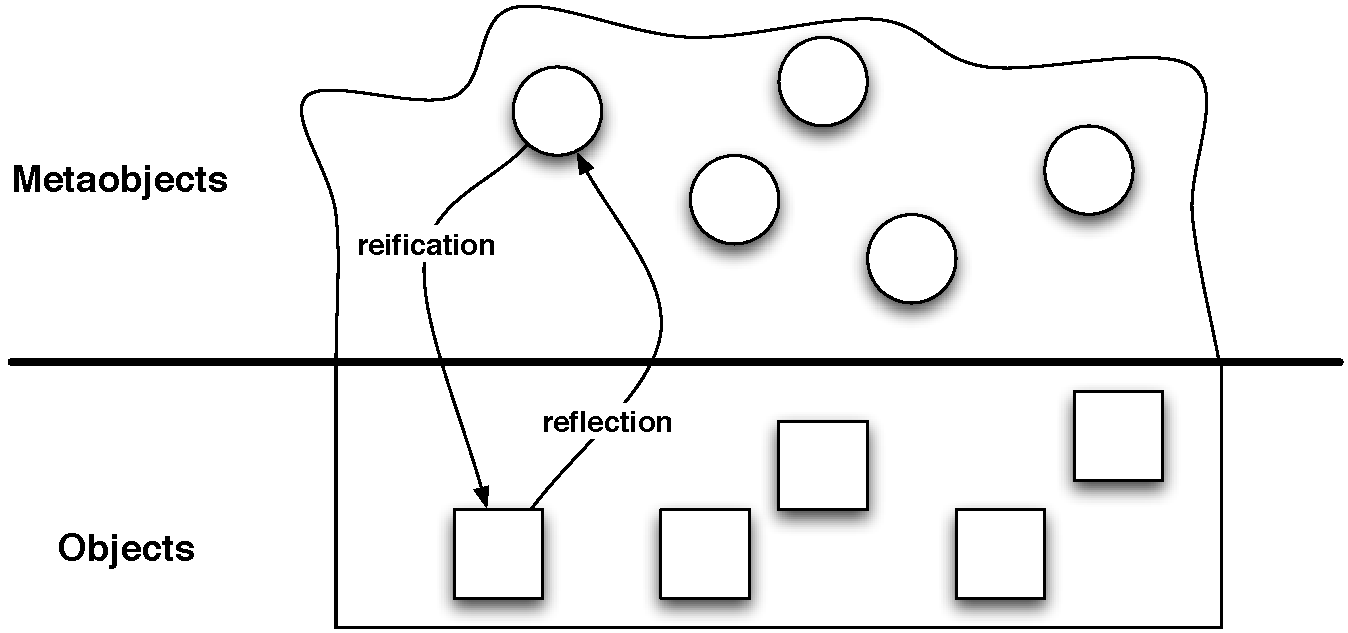
\includegraphics[width=\linewidth]{reflect}
	\caption{Réification et réflexivité.\figlabel{reflect}} % \lr{not referenced, not sure if I understand it}
\end{figure}
Inversement il est possible en \st de modifier les méta-objets réifiés et que leurs modifications soient prises en compte lors de l'exécution du système (voir \figref{reflect}).
Ceci est appelé \emph{intercession} et est principalement utilisé dans les langages de programmation dynamique et de manière plus limitée dans les langages statiques.

Un programme qui manipule d'autres programmes (ou même lui-même) est un \emphind{méta-programme}.
Pour qu'un langage de programmation soit réflexif, il faut qu'il supporte à la fois l'\ind{introspection} et l'\ind{intercession}.

L'introspection est la capacité afin \emph{d'examiner} les structures de données qui définissent le programme comme les objets, classes, méthodes ou pile d'exécution.
L'intercession est la capacité de modifier ces structures, en d'autre terme de changer la sémantique du langage et le comportement d'un programme depuis le programme lui-même.
La \emph{réflexivité structurelle} s'intéresse à l'exploration et à la modification des structures lors du l'exécution du système, alors que la \emph{réflexivité de comportement} concerne l'interprétation de ces structures.

Dans ce chapitre, nous allons principalement nous intéresser à la \ind{réflexivité structurelle}.
Nous illustrerons avec plusieurs exemples pratiques comment \st supporte l'introspection et la méta-programmation.

%======================================
\section{Introspection}

En utilisant un inspecteur, il est possible d'examiner un objet, de changer les valeurs de ces variables d'instances et même de lui envoyer un message.

\dothis{Évaluer le code qui suit dans un workspace:}
\begin{code}{| w |}
w := Workspace new.
w openLabel: 'My Workspace'.
w inspect
\end{code}

Ceci va ouvrir un deuxième workspace et un inspecteur.
L'inspecteur montre l'état interne de ce nouveau workspace : la liste de ces variables d'instances dans la partie gauche (\ct!dependents!, \ct!contents!, \ct!bindings!...) et la valeur de la variable d'instance sélectionnée dans la partie droite.
La variable d'instance \ct!contents! représente ce que le workspace affiche dans sa zone de texte. Ainsi si vous la sélectionnez, la partie droite montrera une chaîne de caractères vide.

\begin{figure}[ht]\centering
	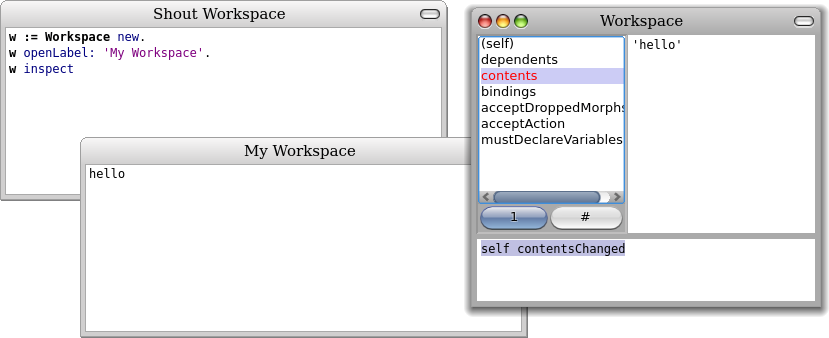
\includegraphics[width=\linewidth]{workspaceInspector}
	\caption{Inspecter un \ct!Workspace!.\figlabel{workspaceInspector}}
\end{figure}

\dothis{Maintenant tapez \ct!'hello'! à la place de la chaîne de caractères vide, puis ensuite faire \emph{accept}.}
La valeur de la variable \ct!contents! change, mais la fenêtre du workspace n'en sera pas notifié, c'est-à-dire qu'elle ne ré-affiche pas son contenu.
Afin d'activer le rafraîchissement de la fenêtre, évaluer \ct!self contentsChanged! dans la partie inférieure de l'inspecteur.

%-----------------------------------------------------------------
\subsection{Accéder aux variables d'instances}

Comment fonctionne l'inspecteur ?
En \st, toutes les variables d'instances sont protégées.
En théorie, il est impossible d'y accéder depuis un autre objet si la classe ne définit pas d'accesseur.
En pratique, l'inspecteur peut accéder aux variables sans avoir besoin d'accesseurs, parce qu'il utilise les capacités réflexives de \st.
En \st, les classes définissent les variables d'instances soient par nom ou au moyen d'indices numériques.
L'inspecteur utilisent des méthodes définies dans la classe \ct!Object! afin d'y accéder :  \lct{instVarAt: \emph{index}} et \lct{instVarNamed: \emph{aString}} peuvent être utilisé pour avoir respectivement la valeur de la variable d'instance à la position \lct{\emph{index}} ou identifié par \lct{\emph{aString}}; pour associer de nouvelles valeurs à ces variables d'instances, on utilise \ct!instVarAt:put:! et \ct!instVarNamed:put:!.
\mthindex{Object}{instVarAt:}
\mthindex{Object}{instVarNamed:}
\mthindex{Object}{instVarAt:put:}
\mthindex{Object}{instVarNamed:put:}

Par exemple, vous pouvez changer la valeur de la variable d'instance \ct!contents! de \ct!w! précédemment définie en évaluant :
\begin{code}{}
w instVarNamed: 'contents' put: 'howdy!'; contentsChanged
\end{code}

\important{\emph{Caveat:} Bien que ces méthodes sont utiles pour construire les outils de l'environnement de développement, les utiliser dans le cadre d'une application conventionnelle est une mauvaise idée: ces méthodes réflexives rompent l'encapsulation des objets et peuvent rendre votre code plus difficile à comprendre et à maintenir.}
% \lr{Why? The access does not show up when looking for all readers/writers in the code browser.}

\ct!instVarAt:! et \ct!instVarAt:put:! sont des \ind{méthodes primitives}, c'est-à-dire qu'elles sont implémentées comme des opérations primitives de la machine virtuelle \pharo.
Si vous consultez le code de ces méthodes, la syntaxe spéciale d'un \ind{pragma} \ct!<primitive: N>! où \ct!N! est un entier.
% \lr{actually this is the syntax of pragmas (method annotations), \ct!primitive:! is just a special kind of pragma}

\needlines{5}
\begin{code}{}
Object>>>instVarAt: index 
	"Primitive. Answer a fixed variable in an object. ..."
	!\textbf{<primitive: 73>}!
	"Access beyond fixed variables."
	^self basicAt: index - self class instSize		
\end{code}

Généralement le code après l'invocation de la primitive n'est pas exécuté. Il est exécuté seulement si la primitive échoue. Dans le cas qui nous intéresse, si on essaie d'accéder à une variable qui n'existe pas, alors le code qui suit la primitive sera essayé. Ceci permet aussi d'utiliser le débogueur sur des méthodes primitives.
Bien qu'il est possible de modifier le code des méthodes primitives, ceci est risqué pour la stabilité de votre image \pharo.

\begin{figure}[ht]\centering
	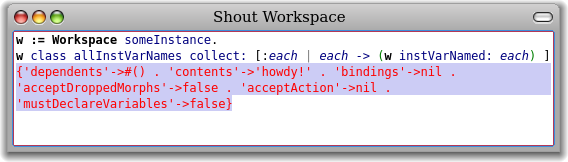
\includegraphics[width=\linewidth]{allInstanceVariables}
	\caption{Afficher toutes les variables d'instance d'un \ct!Workspace!.\figlabel{allInstanceVariables}}
\end{figure}

\figref{AllInstanceVariables} montre comment afficher les valeurs des variables d'instances d'une instance (\ct!w!)  de la classe \ct!Workspace!.
La méthode \ct!allInstVarNames! retourne l'ensemble des noms de variables d'instances d'une classe donnée.

De la même façon, il est possible de collecter les instances qui ont certaines propriétés.
Par exemple, pour avoir toutes les instances de la classe \ct!SketchMorph! dont la variable d'instance \ct!owner! est initialisée avec un morph de type world (\ie les morphs qui sont affichés à chaque instant à l'écran), essayer cette expression:
\begin{code}{}
SketchMorph allInstances select: [:c | (c instVarNamed: 'owner') isWorldMorph]
\end{code}

%-----------------------------------------------------------------
\subsection{Parcourir les variables d'instances}

\mthindex{Object}{instanceVariableValues}
Considérons le message \ct!instanceVariableValues!, qui retourne une collection de toutes les valeurs des variables d'instances définies dans la classe, en excluant les variables d'instances héritées.
Par exemple :
\begin{code}{@TEST}
(1@2) instanceVariableValues --> an OrderedCollection(1 2)
\end{code}

La méthode est implémentée dans \ct{Object} de la manière qui suit :
\needlines{9}
\begin{code}{}
Object>>>instanceVariableValues
	"Answer a collection whose elements are the values of those instance variables of the receiver which were added by the receiver's class."	
	| c |
	c := OrderedCollection new.
	self class superclass instSize + 1
		to: self class instSize
		do: [ :i | c add: (self instVarAt: i)].
	^ c
\end{code}

Cette méthode parcourt par indice les variables d'instances que la classe définit, à partir du dernier index utilisé par les superclasses.
(La méthode \ct!instSize! retourne le nombre des variables d'instances nommées que la classe définit.)

%-----------------------------------------------------------------
\subsection{Faire des requêtes sur les classes et interfaces}

Les outils de développement \pharo (navigateur de code, débogueur, inspecteur, ...) utilisent tous les mécanismes réflexifs que nous avons vu jusqu'à présent.

Voici quelques messages supplémentaires qui peuvent être utile afin de construire des outils de développement :

\lct{isKindOf: \emph{aClass}} retourne vrai si le receveur est une instance de \lct{\emph{aClass}} ou d'une de ces superclasses.
Par exemple :
\begin{code}{@TEST}
1.5 class                     --> Float
1.5 isKindOf: Number --> true
1.5 isKindOf: Integer   --> false
\end{code}
\mthindex{Object}{class}
\mthindex{Object}{isKindOf:}

\lct{respondsTo: \emph{aSymbol}} retourne vrai si le receveur a une méthode dont le sélecteur est \lct{\emph{aSymbol}}.
Par exemple :
\needlines{3}
\begin{code}{@TEST}
1.5 respondsTo: #floor      --> true    "car Number !implémente! floor"
1.5 floor                            --> 1
Exception respondsTo: #, --> true    "exception classes can be grouped"
\end{code}
\mthindex{Object}{respondsTo:}

\important{\emph{Caveat:} Bien que tous ces outils soient particulièrement utiles pour construire des outils de développements, ils ne sont pas appropriés pour une application classique.
Demander à un objet sa classe ou bien l'interroger pour connaître les messages qu'il comprend, sont un signe indiquant une mauvaise conception objet, puisque généralement cela signifie une violation du principe d'encapsulation.
Les outils de développements ne sont pas considérés comme des applications comme les autres, puisque leur domaine d'applications 
Development tools, however, are not normal applications, since their domain is that of software itself. As such these tools have a right to dig deep into the internal details of code.}

%There also exist mechanisms for introspecting on various parts of the run-time system, such as  the process scheduler, the memory manager and so on. For now we will focus on navigating through objects, classes and methods, and we will look more closely at rest of the runtime system in an other chapter.
%\on{let's not mention this if we don't actually write such a chapter!}

%-----------------------------------------------------------------
\subsection{Métriques de code}

Voyons maintenant comment nous pouvons utiliser les mécanismes d'introspection de \st pour rapidement pouvoir construire des métriques de code. Les \ind{métriques} de code mesure certains aspects comme la profondeur de l'arbre d'héritage, le nombre de sous-classes directes ou indirectes, le nombre de méthodes ou de variables d'instances de chaque classe ou enfin le nombre local de méthodes ou de variables d'instances.
Voici quelques résultats de métriques pour la classe \ct!Morph!, qui est la superclasse de tous les objets graphiques de \pharo, révélant qu'il s'agit d'une classe d'une taille conséquente et qu'elle est la racine d'une hiérarchie importante. Peut-être qu'elle nécessiterait d'être refactoriser !

\mthindex{Behavior}{allSuperclasses}
\mthindex{Behavior}{allSelectors}
\mthindex{Behavior}{allInstVarNames}
\mthindex{Behavior}{selectors}
\mthindex{Behavior}{instVarNames}
\mthindex{Behavior}{subclasses}
\mthindex{Behavior}{allSubclasses}
\mthindex{ClassDescription}{linesOfCode}
\begin{code}{}
Morph allSuperclasses size.  -->       2 "profondeur d'!héritage!"
Morph allSelectors size.        --> 1378 "nombre de !méthodes!"
Morph allInstVarNames size. -->      6 "nombre de variables d'instances"
Morph selectors size.             -->  998 "nombre de nouvelles !méthodes!"
Morph instVarNames size.     -->      6 "nombre de nouvelles variables"
Morph subclasses size.          -->    45 "sous-classes directes"
Morph allSubclasses size.      -->  326 "total de sous-classes"
Morph linesOfCode.               --> 5968 "nombre total de lignes de codeBANG"
\end{code}

Une des métriques les plus intéressantes dans le domaine de la programmation par objet est le nombre de méthodes qui étendent les méthodes héritées de la superclasse. Ceci nous informe de la relation entre une classe et ses superclasses.
Dans les prochaines sections, nous verrons comment exploiter notre connaissance des mécanismes d'exécution pour répondre à de telles questions.

%======================================
\section{Parcourir le code}

En \st, tout est objet. Les classes sont en particulier des objets qui fournissent des mécanismes utiles afin de parcourir leurs instances.
La plupart des messages que nous allons voir maintenant sont implémentés dans la classe \ct{Behavior}. Ils sont donc compris de toutes les classes.

Comme nous avons vu précédemment, nous pouvons obtenir une instance particulière d'une classe donnée en lui envoyant le message \ct!#someInstance!.
\mthindex{Behavior}{someInstance}
\begin{code}{@TEST} % Possibly fragile!
Point someInstance --> 0@0
\end{code}

Vous pouvons également rassembler toutes les instances avec \ct!#allInstances! ou déterminer le nombre d'instances en mémoire avec \ct!#instanceCount!.

%\alex{In a Pharo0.1-10342dev09.96.3, I have "ByteString instanceCount --> 63607"}
\mthindex{Behavior}{allInstances}
\mthindex{Behavior}{instanceCount}
\mthindex{Behavior}{allSubInstances}
\begin{code}{} % Cannot test this
ByteString allInstances        --> #('collection' 'position'  ...)
ByteString instanceCount    --> 104565
String allSubInstances size -->  101675
\end{code}

Ces caractéristiques peuvent être très utiles lors du deboguage d'une application, car il est possible de demander à une classe d'énumérer les méthodes possédant des propriétés spécifiques.
\begin{itemize}
\item \mthind{Behavior}{whichSelectorsAccess:} retourne la liste de tous les sélecteurs de méthodes qui lisent ou écrivent dans une variable dont le nom est passé en argument
\item \mthind{Behavior}{whichSelectorsStoreInto:} retourne les sélecteurs des méthodes qui modifient la valeur d'une variable d'instance
\item \mthind{Behavior}{whichSelectorsReferTo:} retourne les sélecteurs des méthodes qui envoie un certain message
\item \mthind{Behavior}{crossReference} associe chaque message avec l'ensemble des méthodes qui l'envoie.
\end{itemize}

\begin{code}{} % TOO FRAGILE TO TEST
Point whichSelectorsAccess: 'x'    --> an IdentitySet(#'\\' #= #scaleBy: ...)
Point whichSelectorsStoreInto: 'x' --> an IdentitySet(#setX:setY: ...)
Point whichSelectorsReferTo: #+  --> an IdentitySet(#rotateBy:about: ...)
Point crossReference --> an Array(
		an Array('*' an IdentitySet(#rotateBy:about: ...))
		an Array('+' an IdentitySet(#rotateBy:about: ...))
		...)
\end{code}

Les messages qui suivent prennent en compte l'héritage :
\begin{itemize}
\item \mthind{Behavior}{whichClassIncludesSelector:} retourne la super-classe qui implémente le message concerné
\item \mthind{Behavior}{unreferencedInstanceVariables} retourne la liste des variables d'instances qui ne sont ni utilisées dans la classe du receveur, ni dans aucune de ses sous-classes
\end{itemize}

\begin{code}{@TEST}
Rectangle whichClassIncludesSelector: #inspect --> Object
Rectangle unreferencedInstanceVariables            --> #()
\end{code}

\clsind{SystemNavigation} is a facade that supports various useful methods for querying and browsing the source code of the system.
\ct{SystemNavigation} \mthind{SystemNavigation class}{default} returns an instance you can use to navigate the system.
Par exemple :

\mthindex{SystemNavigation}{allClassesImplementing:}
\begin{code}{@TEST}
SystemNavigation default allClassesImplementing: #yourself --> {Object}
\end{code}

Les messages suivants devraient être également compréhensibles par eux-même :

\mthindex{SystemNavigation}{allSentMessages}
\mthindex{SystemNavigation}{allUnsentMessages}
\mthindex{SystemNavigation}{allUnimplementedCalls}
\begin{code}{}
SystemNavigation default allSentMessages size          --> 24930
SystemNavigation default allUnsentMessages size      --> 6431
SystemNavigation default allUnimplementedCalls size --> 270
\end{code}

Notons que les messages implémentés mais non envoyés ne sont pas nécessairement inutiles, car ils peuvent être envoyés implicitement (\eg en utilisant \ct{perform:}).
Les messages envoyés mais non implémentés sont plus problématiques, car les méthodes envoyant ces messages vont échoués à l'exécution. Ceci peut être le signe d'une implémentation non finie, d'une API obsolète ou bien de librairies manquantes.

\mthindex{SystemNavigation}{allCallsOn:}
\ct!SystemNavigation default allCallsOn: #Point! retourne tous les messages envoyés explicitement à \ct!Point! comme receveur du message.

All these features are integrated in the programming environment of \pharo, in particular in the code browsers.
As you are surely already aware, there are convenient keyboard shortcuts for browsing all i\underline{m}plementors (\short{m}) and se\underline{n}ders (\short{n}) of a given message.
What is perhaps not so well known is that there are many such pre-packaged queries implemented as methods of the \ct{SystemNavigation} class in the \prot{browsing} protocol.
For example, you can programmatically browse all implementors of the message \ct{ifTrue:} by evaluating:
\mthindex{SystemNavigation}{browseAllImplementorsOf:}
\begin{code}{}
SystemNavigation default browseAllImplementorsOf: #ifTrue:
\end{code}

\begin{figure}[ht]\centering
	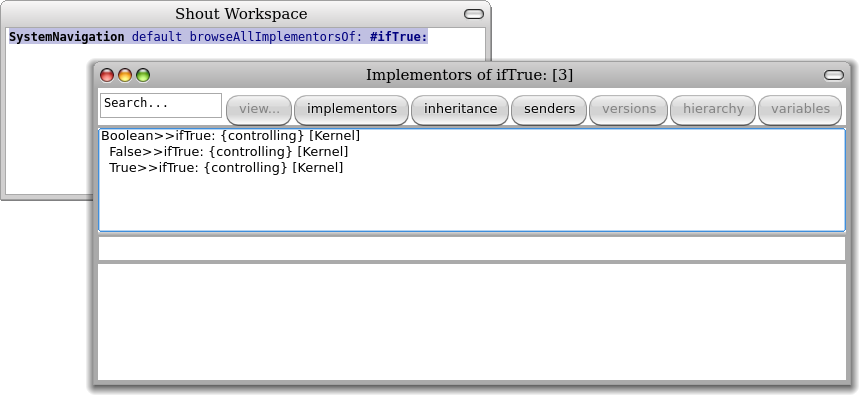
\includegraphics[width=\linewidth]{implementors}
	\caption{Parcourir toutes les implémentations de \ct!\#ifTrue:!.\figlabel{implementors}}
\end{figure}

Particularly useful are the methods \ct{browseAllSelect:} and \lct{browseMethodsWithSourceString:}.  Here are two different ways to browse all methods in the system that perform super sends (the first way is rather brute force; the second way is better and eliminates some false positives):
\mthindex{SystemNavigation}{browseMethodsWithSourceString:}
\mthindex{SystemNavigation}{browseAllSelect:}
\begin{code}{}
SystemNavigation default browseMethodsWithSourceString: 'super'.
SystemNavigation default browseAllSelect: [:method | method sendsToSuper ].
\end{code}

%======================================
\section{Classes, dictionnaires de méthodes et méthodes}

Comme les classes sont des objets, il est possible de les inspecter ou de les explorer de la même manière que les objets.

\mthindex{Object}{explore}
\dothis{\'Evaluer \ct{Point explore}.}

Dans \figref{CompiledMethod}, l' \ind{explorer} montre la structure de la classe \clsind{Point}.
You can see that the class stores its methods in a dictionary, indexing them by their selector.
The selector \ct{#*} points to the decompiled \ind{bytecode} of \ct!Point>>>*!.

\begin{figure}[ht]\centering
	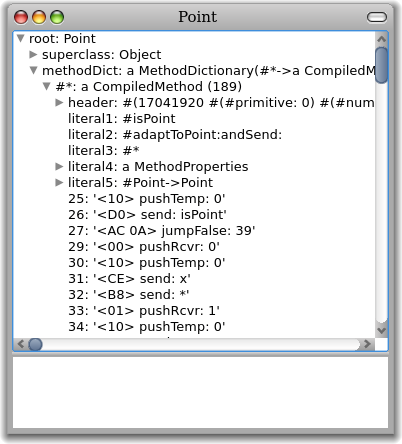
\includegraphics[width=.5\linewidth]{CompiledMethod}
	\caption{Explorer class \ct!Point! and the bytecode of its \ct!\#*! method.\figlabel{CompiledMethod}}
\end{figure}

Examinons la relation entre classes et méthodes.
Dans \figref{MethodsAsObjects} nous voyons que classes et méta-classes ont en commun la superclasse \ct{Behavior}. C'est où la méthode \mthind{Behavior}{new} est définit parmi d'autres méthodes clés pour les classes.
Chaque classe a un dictionnaire de méthode, qui associe chaque sélecteurs de méthodes à des \ind{méthodes compilées}.
Chaque méthode compilée connait la classe dans laquelle elle est installée.
Dans \figref{CompiledMethod}, qu'elle est conservée au moyen d'une association dans \ct{literal5}.

\begin{figure}[ht]\centering
	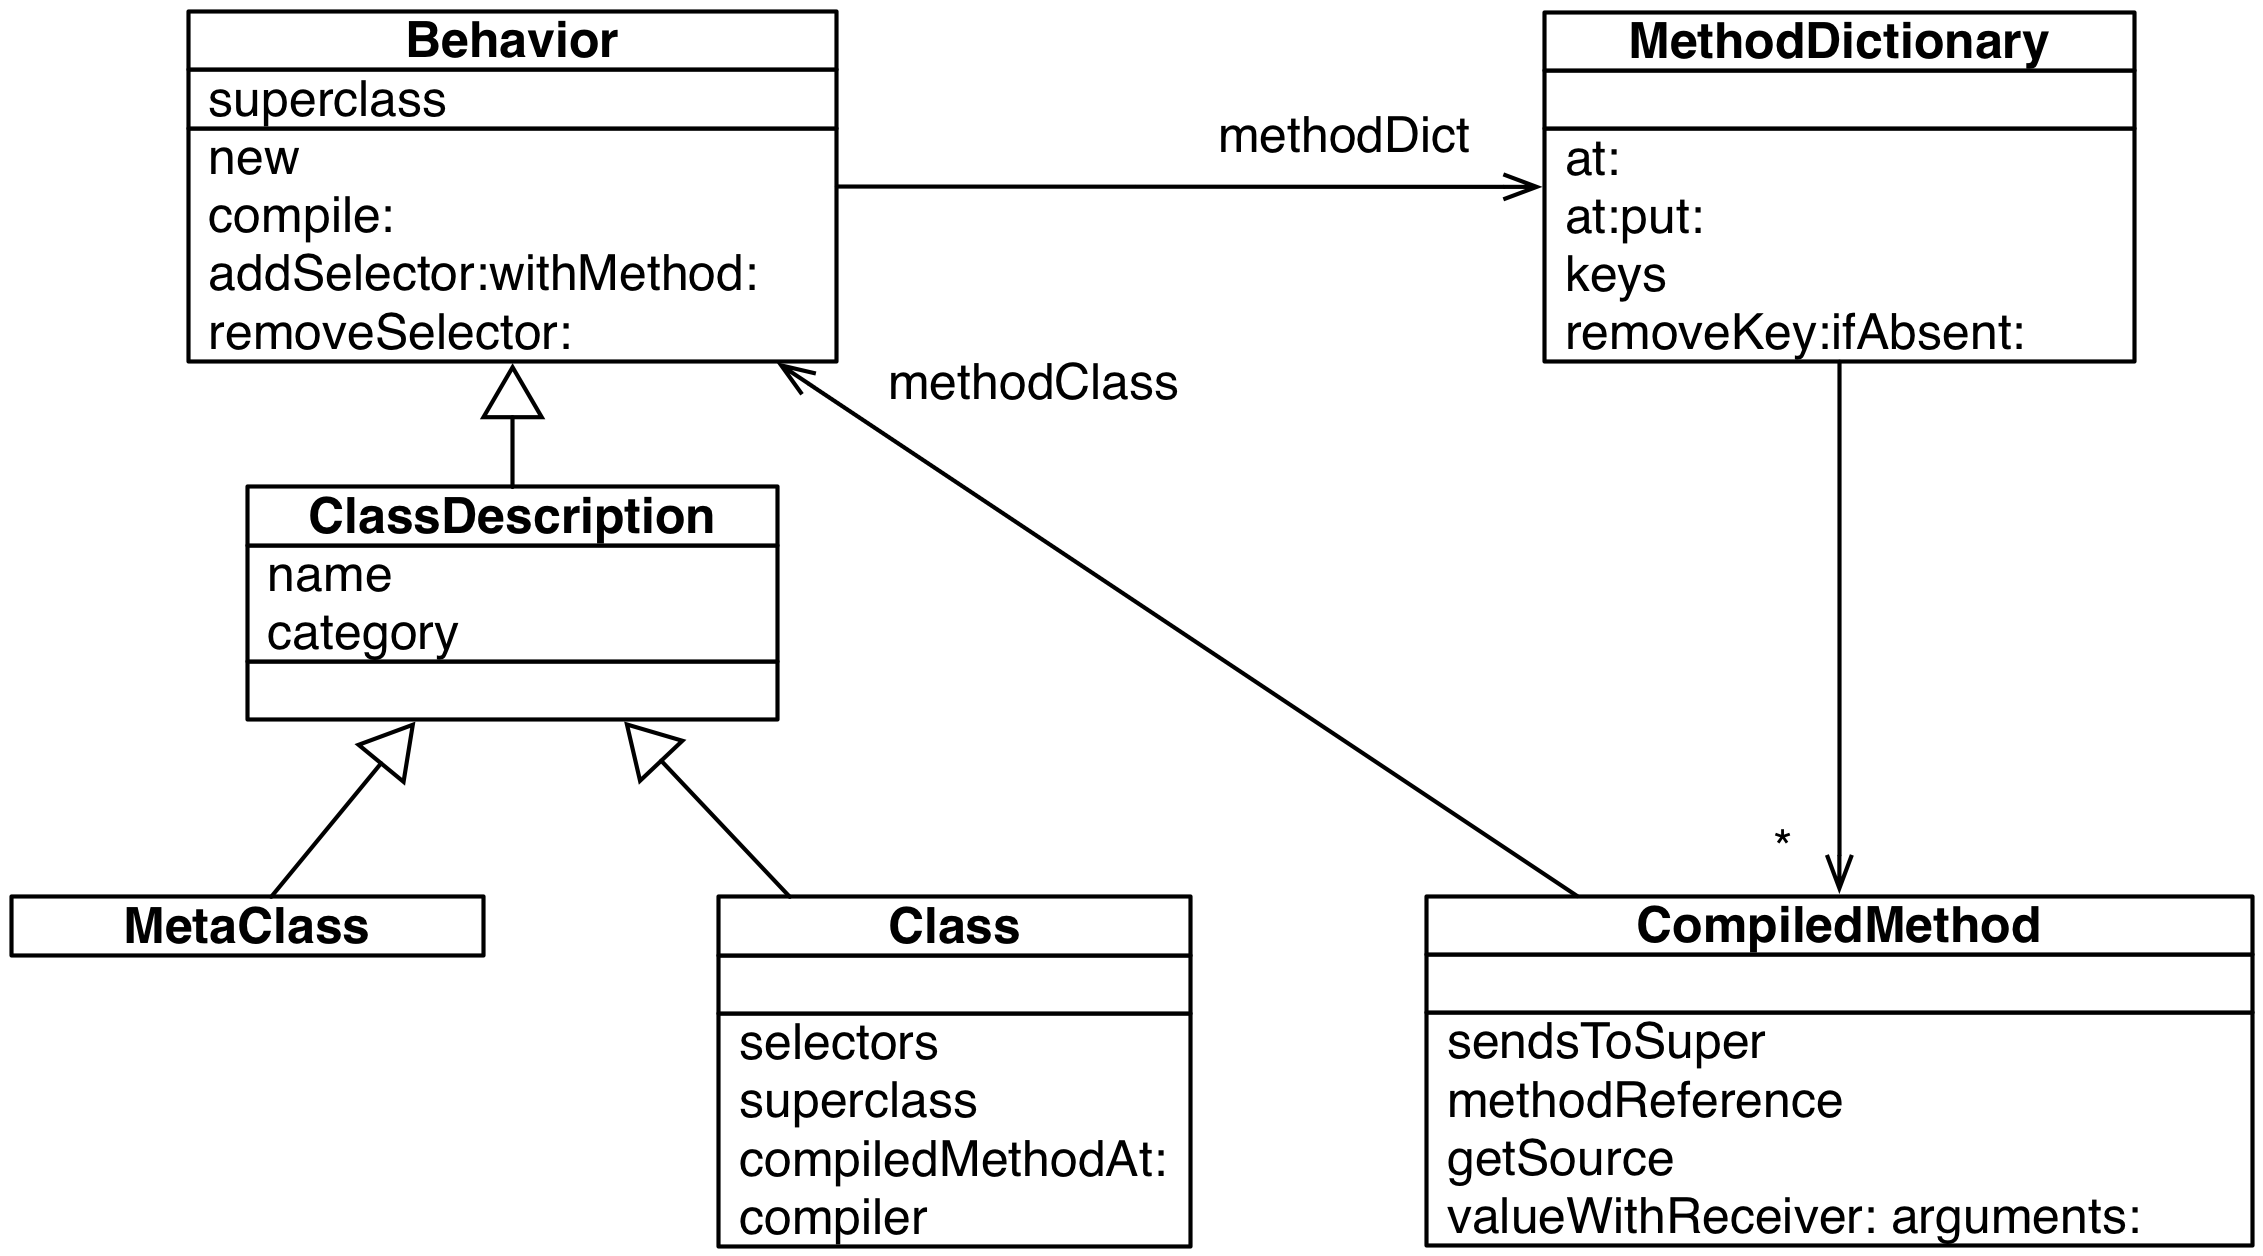
\includegraphics[width=\linewidth]{MethodsAsObjects}
	\caption{Classes, dictionnaires de méthodes et méthodes compilées\figlabel{MethodsAsObjects}}
\end{figure}

On peut exploiter les relations qu'établissent classes et méthdodes, pour effectuer des requêtes sur le système.
For example, to discover which methods are newly introduced in a given class, \ie do not override superclass methods, we can navigate from the class to the \ind{method dictionary} as follows:
\mthindex{Behavior}{methodDict}
\begin{code}{}
[:aClass| aClass methodDict keys select: [:aMethod |
  (aClass superclass canUnderstand: aMethod) not ]] value: SmallInteger
  --> an IdentitySet(#threeDigitName #printStringBase:nDigits: ...)
\end{code}

A compiled method does not simply store the bytecode of a method.
It is also an object the provides numerous useful methods for querying the system.
One such method is \ct{isAbstract} (which tells if the method sends \ct{subclassResponsibility}).
We can use it to identify all the abstract methods of an abstract class
\needlines{4}
\begin{code}{}
[:aClass| aClass methodDict keys select: [:aMethod |
  (aClass>>aMethod) isAbstract ]] value: Number
  --> an IdentitySet(#storeOn:base: #printOn:base: #+ #- #* #/ ...)
\end{code}
Note that this code sends the \ct{>>} message to a class to obtain the compiled method for a given selector.

% As a slightly more complex example, we can browse 

To browse the super-sends within a given hierarchy, for example within the Collections hierarchy, we can pose a more sophisticated query:
\begin{code}{}
class := Collection.
SystemNavigation default
  browseMessageList: (class withAllSubclasses gather: [:each |
    each methodDict associations
      select: [:assoc | assoc value sendsToSuper]
      thenCollect: [:assoc | MethodReference class: each selector: assoc key]])
  name: 'Supersends of ' , class name , ' and its subclasses'
\end{code}
Note how we navigate from classes to method dictionaries to compiled methods to identify the methods we are interested in.
A \ct{MethodReference} is a lightweight proxy for a compiled method that is used by many tools.
There is a convenience method \clsmthind{CompiledMethod}{methodReference} to return the method reference for a compiled method.
\begin{code}{@TEST}
(Object>>#=) methodReference methodSymbol --> #=
\end{code}

%======================================
\section{Environnements de navigation du code}

Although \clsind{SystemNavigation} offers some useful ways to programmatically query and browse system code, there is a better way.  The \ind{Refactoring Browser}, which is integrated into \pharo, provides both interactive and programmatic ways to pose complex queries.

Suppose we are interested to discover which methods in the \lct{Collection} hierarchy send a message to \super which is different from the method's selector.
This is normally considered to be a bad \ind{code smell}, since such a \super-send should normally be replaced by a \self-send. (Think about it --- you only \emph{need} \super to extend a method you are overriding; all other inherited methods can be accessed by sending to \self!)

The refactoring browser provides us with an elegant way to restrict our query to just the classes and methods we are interested in.

\dothis{Open a browser on the class \ct{Collection}.
\actclick on the class name and select \menu{refactoring scope>subclasses with}.
This will open a new Browser Environment on just the \ct{Collection} hierarchy.
Within this restricted scope select \menu{refactoring scope>super-sends} to open a new environment with all methods that perform super-sends within the \ct{Collectuon} hierarchy.
Now \click on any method and select \menu{refactor>code critics}.
Navigate to \menu{Lint checks>Possible bugs>Sends different super message} and \actclick to select \menu{browse}.}

In \figref{sendDifferentSuper} we can see that 19 such methods have been found within the \ct{Collection} hierarchy, including \ct{Collection>>>printNameOn:}, which sends \ct{super printOn:}.
\begin{figure}[ht]\centering
	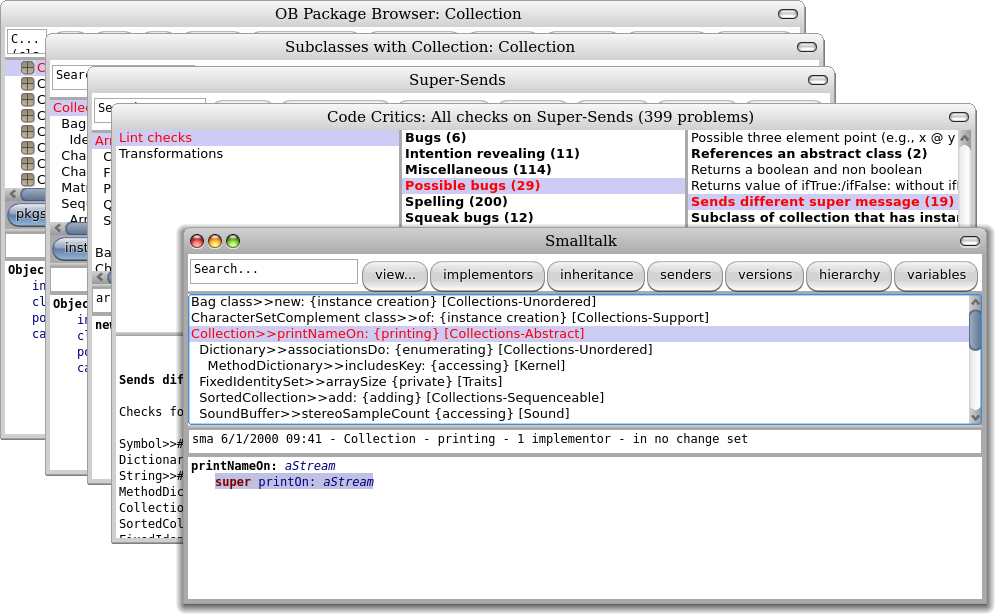
\includegraphics[width=\linewidth]{sendDifferentSuper}
	\caption{Finding methods that send a different super message.\figlabel{sendDifferentSuper}}
\end{figure}

Browser environments can also be created programmatically.
Here, for example, we create a new \clsind{BrowserEnvironment} for \clsind{Collection} and its subclasses, select the super-sending methods, and open the resulting environment.
\needlines{4}
\begin{code}{}
((BrowserEnvironment new forClasses: (Collection withAllSubclasses))
	selectMethods: [:method | method sendsToSuper])
	label: 'Collection methods sending super';
	open.
\end{code}{}

Note how this is considerably more compact than the earlier, equivalent example using \ct{SystemNavigation}.

Finally, we can find just those methods that send a different super message programmatically as follows:
\needlines{6}
\begin{code}{}
((BrowserEnvironment new forClasses: (Collection withAllSubclasses))
	selectMethods: [:method | 
		method sendsToSuper
		and: [(method parseTree superMessages includes: method selector) not]])
	label: 'Collection methods sending different super';
	open
\end{code}
Here we ask each compiled method for its (Refactoring Browser) parse tree, in order to find out whether the super messages differ from the method's selector.
Have a look at the \prot{querying} protocol of the class \ct{RBProgramNode} to see some the things we can ask of parse trees.

%======================================
\section{Accéder au contexte d'exécution}

We have seen how \st's reflective capabilities let us query and explore objects, classes and methods.  But what about the run-time environment?

%-----------------------------------------------------------------
\subsection{Contextes des méthodes}

In fact, the run-time context of an executing method is in the virtual machine --- it is not in the image at all!
On the other hand, the \ind{debugger} obviously has access to this information, and we can happily explore the run-time context, just like any other object.
How is this possible?

Actually, there is nothing magical about the debugger.
The secret is the pseudo-variable \pvind{thisContext}, which we have encountered only in passing before.
Whenever \ct{thisContext} is referred to in a running method, the entire run-time context of that method is reified and made available to the image as a series of chained \clsind{MethodContext} objects.

We can easily experiment with this mechanism ourselves.

\dothis{Change the definition of \ct{Integer>>>factorial} by inserting the underlined expression as shown below:}

\mthindex{Object}{halt}
\begin{code}{}
Integer>>>factorial
	"Answer the factorial of the receiver."
	self = 0 ifTrue: [!\underline{thisContext explore. self halt.}! ^ 1].
	self > 0 ifTrue: [^ self * (self - 1) factorial].
	self error: 'Not valid for negative integers'
\end{code}

\dothis{Now evaluate \ct{3 factorial} in a workspace. You should obtain both a debugger window and an explorer, as shown in \figref{exploringThisContext}.}

\begin{figure}[ht]\centering
	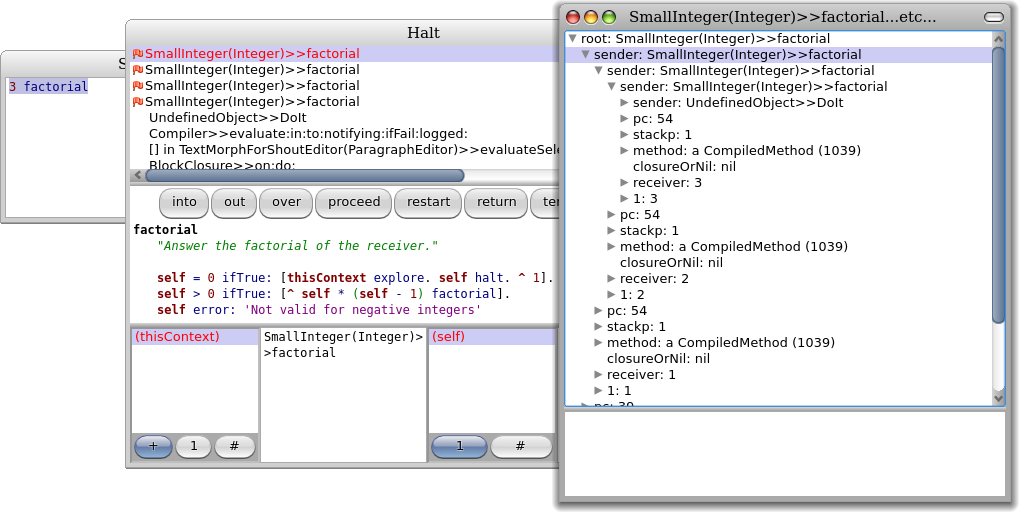
\includegraphics[width=\linewidth]{exploringThisContext}
	\caption{Exploring \lct{thisContext}.\figlabel{exploringThisContext}}
\end{figure}

Welcome to the poor-man's debugger!
If you now browse the class of the explored object (\ie by evaluating \ct{self browse} in the bottom pane of the explorer) you will discover that it is an instance of the class \lct{MethodContext}, as is each \ct{sender} in the chain.
% All of these objects have been created dynamically in the image by the \st virtual machine at the point where \ct{thisContext} was referred to in the \ct{factorial} method. \lr{Not actually. In all the currently available VMs the context objects are created with every method activation, no matter if they are accessed using \ct{thisContext} or not.}

\ct{thisContext} is not intended to be used for day-to-day programming, but it is essential for implementing tools like debuggers, and for accessing information about the call stack.
You can evaluate the following expression to discover which methods make use of \ct{thisContext}:

\begin{code}{}
SystemNavigation default browseMethodsWithSourceString: 'thisContext'
\end{code}

As it turns out, one of the most common applications is to discover the sender of a message.
Here is a typical application:
\begin{code}{}
Object>>>subclassResponsibility
	"This message sets up a framework for the behavior of the class' subclasses.
	Announce that the subclass should have implemented this message."

	self error: 'My subclass should have overridden ', thisContext sender selector printString
\end{code}

By convention, methods in \st that send \ct{self subclassResponsibility} are considered to be abstract.  But how does \clsmthind{Object}{subclassResponsibility} provide a useful error message indicating which abstract method has been invoked?  Very simply, by asking \ct{thisContext} for the sender.

\lr{I think co-routines and continuations should at least mentioned here. Another very practical application that is simple and could be shown here is the ``escaper''. Store the current context into a temp or inst-var \ct{target := thisContext} and jump back to that stack frame at a later point in time using \ct{target return: 123}.}
\sd{lukas maybe we should have another chapter showing such kind of beasts. I would love to read it.
Showing how to use block to build exception and such a kind of point. I think that this chapter should be an introduction may be
we should have a Reflection applied chapter}
\lr{I would love to help writing such a chapter}
%-----------------------------------------------------------------
\subsection{Points d'arrêts intelligents}

\mthindex{Object}{halt}
The \st way to set a breakpoint is to evaluate \ct{self halt} at an interesting point in a method.  This will cause \ct{thisContext} to be reified, and a \ind{debugger} window will open at the breakpoint.
Unfortunately this poses problems for methods that are intensively used in the system.

Suppose, for instance, that we want to explore the execution of \ct{OrderedCollection>>>add:}.
Setting a breakpoint in this method is problematic.

\dothis{Take a \emph{fresh} image and set the following breakpoint:}
\needlines{3}
\begin{code}{}
OrderedCollection>>>add: newObject
	!\underline{self halt.}!
	^self addLast: newObject
\end{code}

Notice how your image immediately freezes!  We do not even get a debugger window.
The problem is clear once we understand that (i) \ct{OrderedCollection>>>add:} is used by many parts of the system, so the breakpoint is triggered very soon after we accept the change, but (ii) \emph{the debugger itself} sends \ct{add:} to an instance of \ct{OrderedCollection}, preventing the debugger from opening!
What we need is a way to \emph{conditionally halt} only if we are in a context of interest.
This is exactly what \clsmthind{Object}{haltIf:} offers.

Suppose now that we only want to halt if \ct{add:} is sent from, say, the context of \ct{OrderedCollectionTest>>>testAdd}.

\dothis{Fire up a fresh image again, and set the following breakpoint:}
\begin{code}{}
OrderedCollection>>>add: newObject
	!\underline{self haltIf: \#testAdd.}!
	^self addLast: newObject
\end{code}

This time the image does not freeze. Try running the \ct{OrderedCollectionTest}.
(You can find it in the \scat{CollectionsTests-Sequenceable} category.)

How does this work?  Let's have a look at \clsmthind{Object}{haltIf:}:
\begin{code}{}
Object>>>haltIf: condition
	| cntxt |
	condition isSymbol ifTrue: [
		"only halt if a method with selector symbol is in callchain"
		cntxt := thisContext.
		[cntxt sender isNil] whileFalse: [
			cntxt := cntxt sender. 
			(cntxt selector = condition) ifTrue: [Halt signal]. ].
		^self.
	].
	...
\end{code}

Starting from \ct!thisContext!, \ct!haltIf:! goes up through the execution stack, checking if the name of the calling method is the same as the one passed as parameter.
If this is the case, then it raises an exception which, by default, summons the debugger.

It is also possible to supply a boolean or a boolean block as an argument to \ct{haltIf:}, but these cases are straightforward and do not make use of \ct{thisContext}.

%======================================
\section{Intercepter les messages non compris}
\seclabel{msgnotunderstood}

So far we have used the reflective features of \st mainly to query and explore objects, classes, methods and the run-time stack. Now we will look at how to use our knowledge of the \st system structure to intercept messages and modify behaviour at run-time.

When an object receives a message, it first looks in the method dictionary of its class for a corresponding method to respond to the message.
If no such method exists, it will continue looking up the class hierarchy, until it reaches \ct{Object}. If still no method is found for that message, the object will \emph{send itself} the message \ct{doesNotUnderstand:} with the message selector as its argument.
The process then starts all over again, until \clsmthind{Object}{doesNotUnderstand:} is found, and the debugger is launched.

But what if \ct{doesNotUnderstand:} is overridden by one of the subclasses of \ct{Object} in the lookup path?
As it turns out, this is a convenient way of realizing certain kinds of very dynamic behaviour. An object that does not understand a message can, by overriding \ct{doesNotUnderstand:}, fall back to an alternative strategy for responding to that message.

Two very common applications of this technique are (1) to implement \ind{lightweight proxies} for objects, and (2) to dynamically compile or load missing code.

%-----------------------------------------------------------------
\subsection{Lightweight proxies}

In the first case, we introduce a ``\ind{minimal object}'' to act as a proxy for an existing object.
Since the proxy will implement virtually no methods of its own, any message sent to it will be trapped by \ct{doesNotUnderstand:}. By implementing this message, the proxy can then take special action before delegating the message to the real subject it is the proxy for.

Let us have a look at how this may be implemented\footnote{You can also load \pkg{PBE-Reflection} from \url{http://www.squeaksource.com/PharoByExample/}}.

We define a \ct{LoggingProxy} as follows:
\begin{code}{}
ProtoObject subclass: #LoggingProxy
	instanceVariableNames: 'subject invocationCount'
	classVariableNames: ''
	poolDictionaries: ''
	category: 'PBE-Reflection'
\end{code}
Note that we subclass \ct{ProtoObject} rather than \ct{Object} because we do not want our proxy to inherit over 400 methods (!) from \ct{Object}.

\begin{code}{}
Object methodDict size --> 408
\end{code}

Our proxy has two instance variables: the \ct{subject} it is a proxy for, and a \ct{count} of the number of messages it has intercepted.
We initialize the two instance variables and we provide an accessor for the message count.
Initially the \ct{subject} variable points to the proxy object itself.
\begin{code}{}
LoggingProxy>>>initialize
	invocationCount := 0.
	subject := self.
\end{code}

\begin{code}{}
LoggingProxy>>>invocationCount
	^ invocationCount
\end{code}

We simply intercept all messages not understood, print them to the Transcript, update the message count, and forward the message to the real subject.
\begin{code}{}
LoggingProxy>>>doesNotUnderstand: aMessage 
	Transcript show: 'performing ', aMessage printString; cr.
	invocationCount := invocationCount + 1.
	^ aMessage sendTo: subject
\end{code}

Here comes a bit of magic.
We create a new \ct{Point} object and a new \ct{LoggingProxy} object, and then we tell the proxy to \mthind{ProtoObject}{become:} the point object:
\seeindex{\ct{become:}}{\ct{ProtoObject>>>become:}}
\begin{code}{}
point := 1@2.
LoggingProxy new !\underline{become:}! point.
\end{code}

This has the effect of swapping all references in the image to the point to now refer to the proxy, and vice versa. Most importantly, the proxy's \ct{subject} instance variable will now refer to the point!

\begin{code}{}
point invocationCount --> 0
point + (3@4)             --> 4@6
point invocationCount --> 1
\end{code}

This works nicely in most cases, but there are some shortcomings:
\begin{code}{}
point class --> LoggingProxy
\end{code}
Curiously, the method \ct{class} is not even implemented in \ct{ProtoObject} but in \ct{Object}, which \ct{LoggingProxy} does not inherit from!
The answer to this riddle is that \ct{class} is never sent as a message but is directly answered by the virtual machine.\footnote{\ct{yourself} is also never truly sent.
Other messages that may be directly interpreted by the VM, depending on the receiver, include:
\ct{+- < > <= >= = ~= * / \ ==}
\ct{@ bitShift: // bitAnd: bitOr:}
\ct{at: at:put: size}
\ct{next nextPut: atEnd}
\ct{blockCopy: value value: do: new new: x y}.
Selectors that are never sent, because they are inlined by the compiler and transformed to comparison and jump bytecodes:
\ct{ifTrue: ifFalse: ifTrue:ifFalse: ifFalse:ifTrue:}
\ct{and: or:}
\ct{whileFalse: whileTrue: whileFalse whileTrue}
\ct{to:do: to:by:do:}
\ct{caseOf: caseOf:otherwise:}
\ct{ifNil: ifNotNil:  ifNil:ifNotNil: ifNotNil:ifNil:}
Attempts to send these messages to non-boolean objects can be intercepted and execution can be resumed with a valid boolean value by overriding \ct{mustBeBoolean} in the receiver or by catching the \ct{NonBooleanReceiver} exception.
}% NB: Notes by Lukas Renggli

Even if we can ignore such special message sends, there is another fundamental problem which cannot be overcome by this approach: \self-sends cannot be intercepted:
\begin{code}{}
point := 1@2.
LoggingProxy new become: point.
point invocationCount --> 0
point rect: (3@4)        --> 1@2 corner: 3@4
point invocationCount --> 1
\end{code}

Our proxy has been cheated out of two \self-sends in the \ct{rect:} method:
\begin{code}{}
Point>>>rect: aPoint 
	^ Rectangle  origin: (self min: aPoint) corner: (self max: aPoint)
\end{code}

Although messages can be intercepted by proxies using this technique, one should be aware of the inherent limitations of using a proxy.  In \secref{wrapper} we will see another, more general approach for intercepting messages.

%-----------------------------------------------------------------
\subsection{Générer des méthodes manquantes}

The other most common application of intercepting not understood messages is to dynamically load or generate the missing methods.
Consider a very large library of classes with many methods.  Instead of loading the entire library, we could load a stub for each class in the library. The stubs know where to find the source code of all their methods.  The stubs simply trap all messages not understood, and dynamically load the missing methods on-demand.  At some point, this behaviour can be deactivated, and the loaded code can be saved as the minimal necessary subset for the client application.

%\on{Stef sez: check ObjectOut -- I looked, but this seems to be very old. Depends on SqueakPage.}

Let us look at a simple variant of this technique where we have a class that automatically adds accessors for its instance variables on-demand:
% \lr{the last statement should return the result of the message, otherwise you cannot proceed with the debugger} \alex{all redefinition of doesNotUnderstand: includes a return statement. However, I do not see your comment lukas, I tried to insert a 'self halt' in the method, I was able to proceed. I added the return in the function} \lr{Of course it depends on the exact circumstances. If you perform a message on self that returns self it does not matter, but in any other case a forgotten return can introduce strange side effects. There was no return in the listing below, but now there is and the problem is solved.}

\begin{code}{}
DynamicAcccessors>>>doesNotUnderstand: aMessage
	| messageName |
	messageName := aMessage selector asString.
	(self class instVarNames includes: messageName)
		ifTrue: [
			self class compile: messageName, String cr, ' ^ ', messageName.
			^ aMessage sendTo: self ].
	^ super doesNotUnderstand: aMessage
\end{code}
Any message not understood is trapped here. If an instance variable with the same name as the message sent exists, then we ask our class to compile an accessor for that instance variables and we re-send the message.

Suppose the class \ct{DynamicAcccessors} has an (uninitialized) instance variable \ct{x} but no pre-defined accessor. Then the following will generate the accessor dynamically and retrieve the value:
\needlines{2}
\begin{code}{}
myDA := DynamicAccessors new.
myDA x --> nil
\end{code}

Let us step through what happens the first time the message \ct{x} is sent to our object (see \figref{DynamicAccessors}).

\begin{figure}[ht]\centering
	\includegraphics[width=\linewidth]{DynamicAccessors}
	\caption{Dynamically creating accessors.\figlabel{DynamicAccessors}}
	% \alex{not sure whether the figure is highly necessary. The code is rather simple and the figure complete to follow in my opinion.}}
	% \on{trust me, it is useful to see all the steps.}
\end{figure}

(1) We send \ct{x} to \ct{myDA}, (2) the message is looked up in the class, and (3) not found in the class hierarchy. (4) This causes \ct{self doesNotUnderstand: #x} to be sent back to the object, (5) triggering a new lookup. This time \ct{doesNotUnderstand:} is found immediately in \ct{DynamicAccessors}, (6) which asks its class to compile the string \ct{'x ^ x'}. The \ct{compile} method is looked up (7), and (8) finally found in \ct{Behavior}, which (9-10) adds the new compiled method to the method dictionary of \ct{DynamicAccessors}. Finally, (11-13) the message is resent, and this time it is found.

The same technique can be used to generate setters for instance variables, or other kinds of boilerplate code, such as visiting methods for a Visitor.

Note the use of \clsmthind{Object}{perform:} in step (13) which can be used to send messages that are composed at run-time:
\begin{code}{@TEST}
5 perform: #factorial                                             --> 120
6 perform: ('fac', 'torial') asSymbol                       --> 720
4 perform: #max: withArguments: (Array with: 6) --> 6
\end{code}

%======================================
\section{Objects as method wrappers}
\seclabel{wrapper}

We have already seen that compiled methods are ordinary objects in \st, and they support a number of methods that allow the programmer to query the run-time system.
What is perhaps a bit more surprising, is that \emph{any object} can play the role of a compiled method. All it has to do is respond to the method \ct{run:with:in:} and a few other important messages.

\dothis{Define an empty class \ct{Demo}. Evaluate \ct{Demo new answer42} and notice how the usual ``Message Not Understood'' error is raised.}

Now we will install a plain \st object in the method dictionary of our \ct{Demo} class.

\dothis{Evaluate \lct{Demo methodDict at: \#answer42 put: ObjectsAsMethodsExample new.}
Now try again to print the result of \ct{Demo new answer42}. This time we get the answer \ct{42}.}

If we take look at the class \clsind{ObjectsAsMethodsExample} we will find the following methods:
%\alex{I would prefer having return 42 in the run:with:in: method, and not having answer42 defined in ObjectsAsMethodsExample, this could be confusing I imagine}
%\on{ObjectsAsMethodsExample is part of the standard pharo image -- it is not in PBE-Reflection}
\needlines{5}
\begin{code}{}
answer42
	^42

run: oldSelector with: arguments in: aReceiver
	^self perform: oldSelector withArguments: arguments
\end{code}

When our \ct{Demo} instance receives the message \ct{answer42}, method lookup proceeds as usual, however the virtual machine will detect that in place of a compiled method, an ordinary \st object is trying to play this role.
The VM will then send this object a new message \ct{run:with:in:} with the original method selector, arguments and receiver as arguments.
Since \ct{ObjectsAsMethodsExample} implements this method, it intercepts the message and delegates it to itself.

We can now remove the fake method as follows:
\begin{code}{}
Demo methodDict removeKey: #answer42 ifAbsent: []
\end{code}

If we take a closer look at \ct{ObjectsAsMethodsExample}, we will see that its superclass also implements the methods \ct{flushcache}, \ct{methodClass:} and \lct{selector:}, but they are all empty.  These messages may be sent to a compiled methods, so they need to be implemented by an object pretending to be a compiled method.  (\ct{flushcache} is the most important method to be implemented; others may be required depending on whether the method is installed using \clsmthind{Behavior}{addSelector:withMethod:} or directly using \clsmthind{MethodDictionary}{at:put:}.)

%-------------------------------------------------------------------------
\subsection{Using methods wrappers to perform test coverage}

Method wrappers are a well-known technique for intercepting messages \cite{Bran98a}.
In the original implementation\footnote{http://www.squeaksource.com/MethodWrappers.html}, a method wrapper is an instance of a subclass of \ct{CompiledMethod}. When installed, a method wrapper can perform special actions before or after invoking the original method.
When uninstalled, the original method is returned to its rightful position in the method dictionary.

In Pharo, \ind{method wrappers} can be implemented more easily by implementing \ct{run:with:in:} instead of by subclassing \ct{CompiledMethod}. In fact, there exists a lightweight implementation of objects as method wrappers\footnote{http://www.squeaksource.com/ObjectsAsMethodsWrap.html}, but it is not part of standard Pharo at the time of this writing.

Nevertheless, the Pharo Test Runner uses precisely this technique to evaluate test coverage.
Let's have a quick look at how it works.

The entry point for test coverage is the method \clsmthind{TestRunner}{runCoverage}:
\begin{code}{}
TestRunner>>>runCoverage
	| packages methods |
	... "identify methods to check for coverage"
	self collectCoverageFor: methods
\end{code}

The method \clsmthind{TestRunner}{collectCoverageFor:} clearly illustrates the coverage checking algorithm:
\begin{code}{}
TestRunner>>>collectCoverageFor: methods
	| wrappers suite |
	wrappers := methods collect: [ :each | TestCoverage on: each ].
	suite := self
		reset;
		suiteAll.
	[ wrappers do: [ :each | each install ].
	  [ self runSuite: suite ] ensure: [ wrappers do: [ :each | each uninstall ] ] ] valueUnpreemptively.
	wrappers := wrappers reject: [ :each | each hasRun ].
	wrappers isEmpty 
		ifTrue: 
			[ UIManager default inform: 'Congratulations. Your tests cover all code under analysis.' ]
		ifFalse: ...
\end{code}
A wrapper is created for each method to be checked, and each wrapper is installed.
The tests are run, and all wrappers are uninstalled.
Finally the user obtains feedback concerning the methods that have not been covered.

How does the wrapper itself work?
The \ct{TestCoverage} wrapper has three instance variables, \ct{hasRun}, \ct{reference} and \ct{method}.
They are initialized as follows:
\begin{code}{}
TestCoverage class>>>on: aMethodReference
	^ self new initializeOn: aMethodReference

TestCoverage>>>initializeOn: aMethodReference
	hasRun := false.
	reference := aMethodReference.
	method := reference compiledMethod
\end{code}

The install and uninstall methods simply update the method dictionary in the obvious way:
\begin{code}{}
TestCoverage>>>install
	reference actualClass methodDictionary
		at: reference methodSymbol
		put: self

TestCoverage>>>uninstall
	reference actualClass methodDictionary
		at: reference methodSymbol
		put: method
\end{code}
\noindent
and the \ct{run:with:in:} method simply updates the \ct{hasRun} variable, uninstalls the wrapper (since coverage has been verified), and resends the message to the original method
\begin{code}{}
run: aSelector with: anArray in: aReceiver
	self mark; uninstall.
	^ aReceiver withArgs: anArray executeMethod: method

mark
	hasRun := true
\end{code}
(Have a look at \clsmthind{ProtoObject}{withArgs:executeMethod:} to see how a method displaced from its method dictionary can be invoked.)

That's all there is to it!

Method wrappers can be used to perform any kind of suitable behaviour before or after the normal operation of a method.  Typical applications are instrumentation (collecting statistics about the calling patterns of methods), checking optional pre- and post-conditions, and memoization (optionally cacheing computed values of methods).

%======================================
\section{Pragmas}

Un \emphind{pragma} est une annotation qui donne des information sur un programme, mais qui n'est pas directement impliqué dans l'exécution de ce programme. Les pragmas n'ont pas d'effet direct lors du déroulement d'une méthode annotée.
Les pragmas sont très utiles notamment pour :
\begin{itemize}
\item Donner de l'information au compilateur : les \indmain{pragmas} peuvent être utilisés par le compilateur pour qu'une méthode appelle une fonction primitive. Cette fonction doit être définie par la machine virtuelle ou au moyen d'un greffon externe.
\item Donner de l'information à l'exécution.
\end{itemize}

Les pragmas s'utilisent uniquement lors de la déclaration des méthodes d'un programme. Une méthode peut déclarer un ou plusieurs pragmas qui sont écrits avant toutes expressions Smalltalk. En réalité, un pragma défini une sorte de message statique avec des arguments qui sont des litéraux.

Nous avons déjà parlé brièvement des pragmas lorsque nous avons briévement introduit la notion de primitives précédemment dans ce chapitre. Une primitive n'est rien moins qu'une déclaration de pragma. 
Consider \ct{<primitive: 73>} as contained in \ct{instVarAt:}. The pragma's selector is \ct{primitive:} and its arguments is an immediate literal value, \ct{73}. 

Le compilateur Smalltalk est probablement l'un des utilisateurs les plus important des pragmas. SUnit is another tool that makes use of annotations. SUnit is able to estimate the coverage of an application from a test unit. One may want to exclude some methods from the coverage. This is the case of the \ct!documentation! method in \ct!SplitJointTest class!:

\begin{code}{}
SplitJointTest class>>>documentation
	<ignoreForCoverage>
	"self showDocumentation"
	
	^ 'This package provides function.... "
\end{code}

By simply annotating a method with the pragma \ct!<ignoreForCoverage>! one can control the scope of the coverage.

%Beside the compiler, Lint is a heavy user of pragmas. Lint is a static code analyzer that flags suspicious, non-portable constructs and code that is likely to contain bugs. It may happen that a method needs to be excluded from Lint analysis. This is the case here:

%\begin{code}{}
%MorphObjectOut>>>doesNotUnderstand: aMessage 
%	"Bring in the object, install, then resend aMessage"
%	"Transcript show: thisContext sender selector; cr."
%	"useful for debugging"
%	
%	! \textbf{<lint: 'Unnecessary "= true"' rationale: 'recursionFlag may be nil' author: 'stephane.ducasse'>}!
%	...
%\end{code}	

%One of the pragmas used by Lint to filter out methods is \ct{lint:rationale:author:}.

As instances of the class \clsind{Pragma}, pragmas are first class objects. A compiled method answers to the message \mthind{CompiledMethod}{pragmas}. This method returns an array of pragmas. 

\begin{code}{@TEST}
(SplitJoinTest class >> #showDocumentation) pragmas
  --> an Array(<ignoreForCoverage>)
(Float>>#+) pragmas --> an Array(<primitive: 41>)
\end{code}

Methods defining a particular query may be retrieved from a class. The class side of \ct!SplitJoinTest! contains some methods annotated with \ct!<ignoreForCoverage>!:

\begin{code}{@TEST}
Pragma allNamed: #ignoreForCoverage in: SplitJoinTest class  --> an Array(<ignoreForCoverage> <ignoreForCoverage> <ignoreForCoverage>)
\end{code}

A variant of \ct{allNamed:in:} may be found on the class side of \ct{Pragma}.

A pragma knows in which method it is defined (using \ct{method}), the name of the method (\ct{selector}), the class that contains the method (\ct{methodClass}), its number of arguments (\ct{numArgs}), about the literals the pragma has for arguments (\ct{hasLiteral:} and \ct{hasLiteralSuchThat:}). 

%\lr{Typically pragmas are performed on an interpreter object that understands the pragma message.}

%======================================
\section{Résumé du chapitre}

Reflection refers to the ability to query, examine and even modify the metaobjects of the run-time system as ordinary objects.

\begin{itemize}
\item The Inspector uses \ct{instVarAt:} and related methods to query and modify ``private'' instance variables of objects.
\item Send \ct{Behavior>>>allInstances} to query instances of a class.
\item The messages \ct{class}, \ct{isKindOf:}, \ct{respondsTo:} \etc  are useful for gathering metrics or building development tools, but they should be avoided in regular applications: they violate the encapsulation of objects and make your code harder to understand and maintain.
\item \ct{SystemNavigation} is a utility class holding many useful queries for navigation and browsing the \ct class hierarchy. For example, use \ct{SystemNavigation default browseMethodsWithSourceString: 'pharo'.} to find and browse all methods with a given source string. (Slow, but thorough!)
\item Every \st class points to an instance of \ct{MethodDictionary} which maps selectors to instances of \ct{CompiledMethod}. A compiled method knows its class, closing the loop.
\item \ct{MethodReference} is a leightweight proxy for a compiled method, providing additional convenience methods, and used by many \st tools. 
\item \ct{BrowserEnvironment}, part of the Refactoring Browser infrastructure, offers a more refined interface than \ct{SystemNavigation} for querying the system, since the result of a query can be used as a the scope of a new query. Both GUI and programmatic interfaces are available.
\item \ct{thisContext} is a pseudo-variable that reifies the run-time stack of the virtual machine. It is mainly used by the debugger to dynamically construct an interactive view of the stack. It is also especially useful for dynamically determining the sender of a message.
\item Intelligent breakpoints can be set using \ct{haltIf:}, taking a method selector as its argument. \ct{haltIf:} halts only if the named method occurs as a sender in the run-time stack.
\item A common way to intercept messages sent to a given target is to use a ``minimal object'' as a proxy for that target. The proxy implements as few methods as possible, and traps all message sends by implementing \ct{doesNotunderstand:}. It can then perform some additional action and then forward the message to the original target.
\item Send \ct{become:} to swap the references of two objects, such as a proxy and its target.
\item Beware, some messages, like \ct{class} and \ct{yourself} are never really sent, but are interpreted by the VM.  Others, like \ct{+}, \ct{-} and \ct{ifTrue:} may be directly interpreted or inlined by the VM depending on the receiver.
\item Another typical use for overriding \ct{doesNotUnderstand:} is to lazily load or compile missing methods.
\item \ct{doesNotUnderstand:} cannot trap \self-sends.
\item A more rigorous way to intercept messages is to use an object as a method wrapper. Such an object is installed in a method dictionary in place of a compiled method. It should implement \ct{run:with:in:} which is sent by the VM when it detects an ordinary object instead of a compiled method in the method dictionary. This technique is used by the SUnit Test Runner to collect coverage data.
\end{itemize}

%=========================================================
\ifx\wholebook\relax\else
   \bibliographystyle{jurabib}
   \nobibliography{scg}
   \end{document}
\fi
%=========================================================

%Other stuff:
%- anonymous classes (uses compile: and primitiveChangeClassTo:) ???
%- collect direct senders; class collaborations
%- Object primitiveChangeClassTo: become: and becomeForward: (see tests and slides with minimal object example)
%- PointerFinder?
%- anonymous classes (see slides) ?

%Test  Coverage using ObjectsAsMethodsWrap package:
%\begin{code}{}
%category := 'SCGPier'.
%w := (ObjectAsOneTimeMethodWrapper installOnClassCategory: category).
%tr := TestRunner new.
%ToolBuilder open: tr.
%[tr
%	categoryAt: (tr categoryList indexOf: 'SCGPier') put: true;
%	selectAllClasses;
%	runAll.]
%ensure: [[w do: [:each| each uninstall ]] valueUnpreemptively].
%((w select: [:each | each executed not ])
%	collect: [:each | each wrappedClass name, '>>', each selector name ]) explore.
%\end{code}
